\documentclass[titlepage, 12pt]{article}
\usepackage[utf8]{inputenc}
\usepackage{authblk}
\usepackage{blindtext}
\usepackage[bibstyle=numeric, citestyle=numeric, backend=biber, sorting=none]{biblatex}
\usepackage{graphicx}
\usepackage{hyperref}
\usepackage[letterpaper, margin=1in, left=1.5in]{geometry}
\usepackage{helvet}
\usepackage{url}
\usepackage[T1]{fontenc}
\usepackage{csvsimple}
\usepackage{tabularx}
\usepackage{booktabs}
\usepackage{graphicx}
\usepackage{caption}
\usepackage{subcaption}
\usepackage{multirow}
\usepackage{listings}
\usepackage{adjustbox}
\usepackage{appendix}
\usepackage{amsmath}
\usepackage{array}

\newcolumntype{L}{>{\centering\arraybackslash}m{5cm}}
\newcolumntype{S}{>{\centering\arraybackslash}m{2cm}}
\newcolumntype{M}{>{\centering\arraybackslash}m{7cm}}

\DeclareMathOperator{\round}{round}

\renewcommand{\familydefault}{\sfdefault}

\hypersetup{
    colorlinks,
    citecolor=black,
    filecolor=black,
    linkcolor=black,
    urlcolor=black
}

\lstset{
frame = single, }

\lstdefinelanguage{JavaScript}{
  morekeywords=[1]{break, continue, delete, else, for, function, if, in,
    new, return, this, typeof, var, void, while, with},
  % Literals, primitive types, and reference types.
  morekeywords=[2]{false, null, true, boolean, number, undefined,
    Array, Boolean, Date, Math, Number, String, Object},
  % Built-ins.
  morekeywords=[3]{eval, parseInt, parseFloat, escape, unescape},
  sensitive,
  morecomment=[s]{/*}{*/},
  morecomment=[l]//,
  morecomment=[s]{/**}{*/}, % JavaDoc style comments
  morestring=[b]',
  morestring=[b]"
}[keywords, comments, strings]

\title{MIDI Autofill}
\author[1]{Samantha Del Rosario}
\author[1]{Mason Ashbridge}
\author[1]{Jorge D. Fochezato}
\author[2]{Eric Franklin}
\author[2]{Brian Smith}
\affil[1]{CS Group 14}
\affil[2]{ECE Group 27}

\date{Spring 2021}

\addbibresource{references.bib}

\begin{document}

\pagenumbering{roman}

\setlength{\parskip}{1em}
\setlength{\parindent}{0cm}

\patchcmd{\titlepage}
{\thispagestyle{empty}}
{\thispagestyle{plain}}
{}
{}

\maketitle

\newpage
\setcounter{page}{2}
\tableofcontents
\newpage

\pagenumbering{arabic}

\input{executivesummary.tex}
\section{Project Overview}
\subsection{Function of the Project}

The final product of this project should serve as a music production and music
education tool. The keyboard itself will allow the user to interactively experiment with
writing melodies, and the autofill feature will assist in expanding the user’s capability.
For music production it can kickstart the writing process, allowing a smooth and
constant flow of ideas and creativity, thereby boosting the productivity of the user.
For music education it can, through demonstration, teach stylistic patterns and
structures that the user can mimic in their own writing to create a similar sound.

The product should also simply serve as a tool of convenience. Musical practitioners often find
that it can be inconvenient to even begin a music writing or practice session, because a lot of the
necessary equipment is cumbersome or complex, requiring time to transport and set up. Smaller
instruments such as the ukulele are enjoyed particularly for their simplicity and mobility, because
it makes spontaneous bouts of music more achievable. The MIDI Autofill keyboard should fill a
similar niche in the music production community by providing more simplified functionality to a
synthesizer production set up in exchange for ease of learning and ease of use.

\subsection{Design Criteria}

Aside from achieving base functionality, there are few requirements regarding the
product’s design. Its keys should be aesthetically and structurally reminiscent of a
piano, to make for more intuitive use. Additionally, the visualization of the melody in
the DAW should follow the horizontal bar format seen in most standard MIDI editors.

The standalone design makes music production more convenient, as producers often have to have
several devices connected to each other as well as to their own power sources to have complete
utility. Because this is a key benefit of the MIDI Autofill Keyboard, our features should be
designed to enhance that mobility. A small, light-weight body will allow the user to transport it
easily. Low dependency on external power sources will also expand the variety of use by not
requiring a nearby outlet.

\subsection{Constraints}
\label{sec:constraints}

The primary constraint of this project will be hardware. Both the AI model and Digital
Audio Workstation will need to be operating without the assistance of external
processing power. Additionally, we hope to make this product affordable. To meet
these needs, we will need to strike a balance between the complexity of the software
and the capabilities of decently priced hardware.

Other constraints include budget and time. Because this project is slotted for the spring and
summer semesters, it will have to take place over a more condensed timeline. On top of that, the
team will experience limited contact in the interest of public health in the current state of the
COVID-19 pandemic. Understanding these factors, the scope of this project has been designed for
flexibility. We ensured that the minimum viable product is within an acquirable skill set, so that
 it may be achieved quickly and with few complications. At the same time, we have an expansive list
  of optional features that would improve function and enhance the technical level of the project
  if we have the time to implement them. With this structure, we have confidence in our ability to
  produce a working model within our time constraints even during restrictive circumstances but
  also plenty of room to exercise a higher level of technical achievement if time permits.

\subsection{Legal, Ethical, and Privacy Issues}

\subsubsection{Legal}

Copyright of AI generated works is a highly debated issue. It is a common legal opinion
that AI generated works cannot be copyrighted, as they are not a human creative
expression, but there is no legal precedent on this matter that we are aware of. In our
case, the AI is not generating entire works, but is a tool in a human's creative process.
We believe that in our case the end-user would still retain copyright for their work.
We may want to include a clause in our license that specifically states that the end-user
will own the copyright to their generated works. This can hopefully clear up any concerns
to the end-user about ownership and would give users confidence that they can freely use
our device without copyright concerns.

The source code of the model and any other libraries we use should be an open source and
permissive license. Licenses such as MIT and Apache would be more ideal than a copyleft
license, such as the GPL. The GPL is particularly bothersome, as even if we do make our
code open source, it is easy to unintentionally violate the GPL. Even the Free Software
Foundation, who authored the GPL, has accidentally violated the GPL before with it's GNU
Emacs software, when they distributed binary blobs without the source code
\autocite{emacsGplViolation}. Our policy is to avoid the GPL in all dependencies. If we do
end up needing to rely on GPL code, then we should sandbox it off into a small program
that we release separately under a GPL license.

One of the AI libraries we are evaluating, Magenta, uses the Apache 2.0 License, which is
great for us. This license will be easy to comply with, as we simply need to include a
copy of the license with our code and state if there are any modifications to the code.
That is just one example, but it will be important for us to audit the licenses of all our
dependencies before distribution to be sure we comply. We are using JavaScript with
NodeJS, which means we have hundreds of indirect dependencies which we need to audit. We
are using a NodeJS program called \url{license-checker} to audit the license of our
dependencies, and only allowing the MIT, BSD, and Apache licenses.

Another area of concern is the copyright of the pretrained model. It is debatable whether
a pretrained model can even be copyrighted. It would need to be considered an act of
human creative expression, and the pretrained models arguably not the result of a creative
process. These models are freely distributed online, and it would be hard to argue that
they are not intended to be used freely, but we should still verify that we have license
to use and distribute it. The pretrained models would likely not be included in the code
repository and could be subjected to a different license. For this project, we will need
the ability to distribute copies of the pretrained model. We may even have multiple
pretrained models per genre if we accomplish our stretch goal of multiple genres/artists.
In such a case we will need to verify the license of all models for each genre. If we
cannot find a pretrained models that fits this requirement, then we may need to train our
own model. If the source code of the model has a permissive license then it should not be
an issue for us to train our own model for distribution, should that be necessary.

\subsubsection{Ethical}

There are also many questions about the ethics of AI generated artwork. This is a highly
opinionated topic, with many people who are fearful of AI. Many feel great concern that
not only does AI have the potential to substitute labor, but also artistic endeavors. Some
who have thought that art would be safe from AI are shocked to see that AI currently can
produce interesting and thought-provoking art. While it will still be a long time for AI
to catch up with human creativity, it is not a misplaced concern. With that said, we
believe that this project does not fall into this category of AI, as it is intended as a
tool to assist musicians rather than to replace artistic talent. The project’s goal is not
to replace the musician, but to help foster their creativity. The MIDI autofill function
will only continue an existing melody, not generate an entirely new one.

\subsubsection{Privacy}

As far as privacy goes, it is a mostly a non-issue for this project, provided our
implementation is correct. We have no server-side component, and no plans to track any
user data. The MIDI device will not require any public network connectivity and will not
store personally identifiable information.

The microcontroller we are using, the Raspberry Pi 4B, does have networking capability,
and we need local networking capability for the USB connection (which works over normal
networking interfaces in our case) and potentially for any interprocess communication.
But we are taking extra steps to ensure that any public networking is disabled so that the
device cannot get compromised through network. Although it would be a bit of a stretch, if
the host machine can be compromised through the MIDI device, then that could lead to major
privacy violations.

\subsection{Broader Impacts}

One of the most difficult aspects of producing music as a hobby is a lack of
accessible equipment. Often, it requires several pieces of hardware at over \$100
each as well as licensed software to compose a polished track. This expensive
and convoluted process restricts the reach of music production as an art. As
technology expands into the music production world, the art becomes more
accessible to the everyday person, and the MIDI Autofill keyboard will be yet
another step along that path. With recording, editing, and auto-completion all
conveniently packaged into a single portable piece of equipment, novice
producers can begin completing polished tracks without having to seek out,
invest in, and store a stockpile of hardware.

Additionally, the autofill feature can benefit new practitioners and
professionals alike. One of the biggest stressors in songwriting is writer’s
block -– it can completely bottleneck the production process and halt all
progress until resolved. For beginners this can be frustrating and discourage
further exploration into the art, and for professionals this can come at the
detriment of deadlines. The melody autofill feature can provide inspiration or
even an immediate solution, expediting the process and allowing artists to be
more productive with their ideas. The goal is to empower independent creators
because the more people can express themselves through art, the richer and more
diverse our culture and society become.

\section{Specifications and Requirements}

\subsection{DAW Integrated Keyboard}

This project aims to create a complete MIDI controller with an integrated and complete
Digital Audio Workstation(DAW) in the system. The DAW will be able to interact with the
user via the keyboard, which acts as the MIDI controller, and can export a completed MIDI
file to a third party computer. For stability purposes, a more refined material will
likely be acquired to use in our final design while printed products will be utilized for
prototyping and visualization purposes.

This printed product will need to be created in sections to allow for printing from a
smaller 3D printing platform, but such a feature is easily designed around and is a common
tactic for printing much larger projects than the printer is normally capable of, but
sizable enough to house the necessary electrical components for our project.

The DAW itself will be hosted on an on board computer and be utilized to enact and execute
the various other features that are mentioned in this section and the document as a whole.
These features are subject to change and the exact method of execution will also likely
change to best accommodate our update in available information. Upon my writing this, we
have already been informed of a more preferential AI software to utilize for our system as
well as a handful of other AI that already exist that could be utilized in our project.
There is no telling where this project will lead us. Only time will tell.

\subsection{Autofill}

The Autofill feature should be capable of receiving a MIDI sequence as input, and producing
a new MIDI sequence which concatenates AI-generated MIDI notes to the end of the input sequence.
The AI should produce notes from the same scale as the input at least 90% of the time. It should
also produce notes within a perfect fifth interval (seven semitones) of the preceding note 90% of
the time. This will maintain the conjunctness of the melody - further discussed in \textbf{\ref{sec:theory} \nameref{sec:theory}}.

As a stretch goal, this feature should be able to implement influence's from the player's own style
by occasionally imitating melodic and/or rhythmic patterns from the input.

\subsection{Battery Life}

The device will be able to remain operational for six hours disconnected to any given
power supply. This will allow the user to change location and find a place of inspiration
before composing a musical piece. This will also encourage us to prioritize processor
usage to ensure that no overuse of resources or space occurs on our internal system. The
battery life will likely come in the form of internal packs that can be charged and
discharged depending on the requirements of the user as well as the power modes for the
internal computer.

Energy efficiency will be critical as well considering much of the pollution that occurs
in the world is due to runoffs from lithium mining and such materials in the soil have a
harsh environmental impact so limiting our required batteries while maximizing our battery
life is and absolute must in the situation.

\subsection{Energy Consumption}

The device will consume no more than 12 watts in a given moment. This will allow for an
extended battery life to longer times and mitigate the environmental impact of the MIDI
controller. This will also force us to limit the energy consumption via efficiency methods
and further allow our previous goal of battery life to come to fruition.

The consumption of energy also carries an environmental weight so limiting the amount of
energy our construction produces will help prevent the waste of electrical resources or
battery integrity.

\subsection{Processing Time}

The time it takes to compute a given function will take no longer than 5 seconds, limiting
user frustration upon perceived lag. This will also force an efficient solution to the
Energy consumption problem as the longer the device uses the main computing unit the more
power it will consume. Such computing problems happen on a near consistent basis and
utilizing optimization will be an essential technique in any field of computer science or
engineering.

This requirement will also force us to think creative when utilizing and implementing the
AI as these programs are notoriously tricky and time consuming, both to train and to
implement properly.

\section{Research}

\subsection{Music Technology}

\subsubsection{MIDI}

MIDI stands for Musical Instrument Digital Interface, and it is used to communicate music
to computers in separate parts. MIDI files themselves do not contain any audio. Instead,
they send system and channel messages. Each message describes several features, but in
this project we are primarily concerned with note ON/OFF and the timing clock. The note
ON/OFF tells which notes are playing during a certain event and at what velocity. The
timing clock keeps track of when each event is scheduled to occur.

Between these two features we can determine pitch, timing, and expression - the three
components of a note which determine whether or not it is melodic in context.

\subsubsection{DAW}
\label{sec:daw}

DAW stands for Digital Audio Workstation. DAWs are the software that provide an interface
through which users can alter the contents of a MIDI or other audio file. Because our DAW
is to be isolated to a MIDI controller, it  will only contain functions concerning MIDI
data. When dealing with MIDIs, DAWs visualize audio in a piano roll display. The
foundation of the piano roll is a set of rows, each one representing a piano key and its
corresponding note. The horizontal axis represents the timing clock data. For each note
that plays in the MIDI, the piano roll displays a colored bar located in the row of the
corresponding note and spanning the length of the corresponding timing clock data.
Additionally, some DAWs show the velocity of the note by the color of the bar - most
commonly, red denotes high velocity while blue/violet denotes low velocity.

\begin{figure}[h!]
  \centering
  \includegraphics{image/PianoRoll.png}
  \caption{Example of a piano roll display}
  \label{fig:piano_roll}
\end{figure}

The most basic ways a DAW can alter a MIDI are by adding, deleting, and editing notes on
the piano roll; users can change the timing, pitch, and/or velocity of any note. DAWs can
also quantize notes, meaning they will automatically shift the timing of the notes so that
every note begins on some specified fraction of the tempo (most commonly a thirty-second
note). This function is especially useful in adjusting for human errors in timing when
writing MIDIs with a MIDI controller. Better timing makes it easier to synchronize with
other tracks that might end up in the same audio file.

\subsection{Music Theory: Melody}

One of the biggest issues with creating computer-generated music is that music, like all art
forms, is highly subjective. There are no universal rules for right or wrong, and yet at the
same time there are combinations of sound that could (almost) universally be considered bad music.
So how does a computer decide what factors will most likely lead to a good melody?

To start, the generally agreed upon definition of melody is that it is the linear succession
of musical tones, with its primary components being pitch and rhythm. Occasionally, it also
encompasses tonal color and other factors of expression.\autocite{melody} In music theory, parts
of music can be described as dissonant or consonant. Dissonance denotes a feeling of tension or
incompleteness in a musical phrase, and consonance denotes resolution and stability. Once again,
these metrics are highly subjective, but they are based in the principle that music is composed
of organized patterns in sound.\autocite{musiciansArithmetic} Aside from easily identifiable
patterns, such as rhythm or repeated note sequences, this especially applies to patterns in note
intervals. In the following subsections, we will discuss a few of the measures we could use to
qualitatively measure the success of our AI output.

\subsubsection{Degrees}

A basic pre-requisite as to whether or not a note is considered tonally consonant is whether or
not it comes from the same scale and key as its context. Western music is traditionally tuned to
the twelve-tone equal temperament (12TET). This tuning is where you get the twelve-note octave
with seven natural tones - the exact same one which is reflected in the configuration of piano keys
which have a repeating pattern consisting of seven white and five black keys. The seven natural
tones make up the diatonic scale. Each tone in the scale can also be called by its degree, i.e.
its role in the scale based on its scale step from the root note.

\begin{table}[h!]
  \centering
  \resizebox{\textwidth}{!}{%
    \begin{tabular}{|S|M|M|S|}
      \hline
      Degree             & Name                                  & Meaning                                                                                        & Note (in C major) \\ \hline
      1                  & Tonic                                 & Tonal center, note of final resolution                                                         & C                 \\ \hline
      2                  & Supertonic                            & One whole step above the tonic                                                                 & D                 \\ \hline
      3                  & Mediant                               & Midway between tonic and dominant, (in minor key) root of relative major key                   & E                 \\ \hline
      4                  & Subdominant                           & Lower dominant, same interval below tonic as dominant is above tonic                           & F                 \\ \hline
      5                  & Dominant                              & Second in importance to the tonic                                                              & G                 \\ \hline
      6                  & Submediant                            & Lower mediant, midway between tonic and subdominant, (in major key) root of relative minor key & A                 \\ \hline
      \multirow{2}{*}{7} & Subtonic (in the natural minor scale) & One whole step below tonic in natural minor scale.                                             &                   \\ \cline{2-4}
                         & Leading tone (in the major scale)     & One half step below tonic. Melodically strong affinity for and leads to tonic                  & B                 \\ \hline
      1                  & Tonic (octave)                        & Tonal center, note of final resolution                                                         & C                 \\ \hline
    \end{tabular}}
  \caption{The names and meanings of each degree in the diatonic scale}
  \label{Tab:degrees}
\end{table}

According to music theory, each degree plays a different role in the scale based on its generation
or release of tension. The tonic, for example, is colloquially known as "home" in the scale,
because it is where most music starts and where most music can resolve and conclude to. In other
words, it is a universal vehicle for tension release. The subtonic or leading tone is named as
such because within the scale it sounds unstable on its own and often relies on the tonic to resolve
it. Thus the subtonic plays the opposite function to the tonic in that it is a universal tension
generator. Good melodies are constructed not to avoid generating tension, but to end the
musical phrase with an equal release of tension.

By being aware of the role of each note in a scale we can get a sense not only of whether or not
the AI-generated outputs are sufficiently competent in melodic structure, but also why that is so.

\subsubsection{Harmonics}

Scales are not the only markers for tonal intervals. Another factor that plays a role in the
consonance of pitch is harmonics. The Lipps-Meyer law, for example, proposes that the consonance
of a melodic interval can generally be determined by whether or not the end tone of the interval
can be represented by a power of two.\autocite{musiciansArithmetic} These numbers which represent
the tones are not their scale intervals, but instead are derived from the Harmonic Series.

The Harmonic Series is actually based on a principle in physics. Sound is a wave, any tone $ t $
is a sound wave oscillating at a specific frequency $ f $. Any sound wave with a frequency
that is an integer multiple of $ f $ is considered to be harmonic to $ t $.\autocite{intervals} For example,
if $ f $ is the frequency of the tonic (the root note of a scale), the unison (no interval,
so also the root note) would be the first harmonic because it has the same frequency. The second
harmonic has a frequency of $ 2/f $ - this coincides with the tone that's exactly one octave
above the root. In fact, every power of two falls on the root note of a different octave. Going
back to the Lipps-Meyers law, this implies that proper consonance can be achieved by ending the
musical phrase on the tonic of the key.

\begin{figure}[h!]
  \centering
  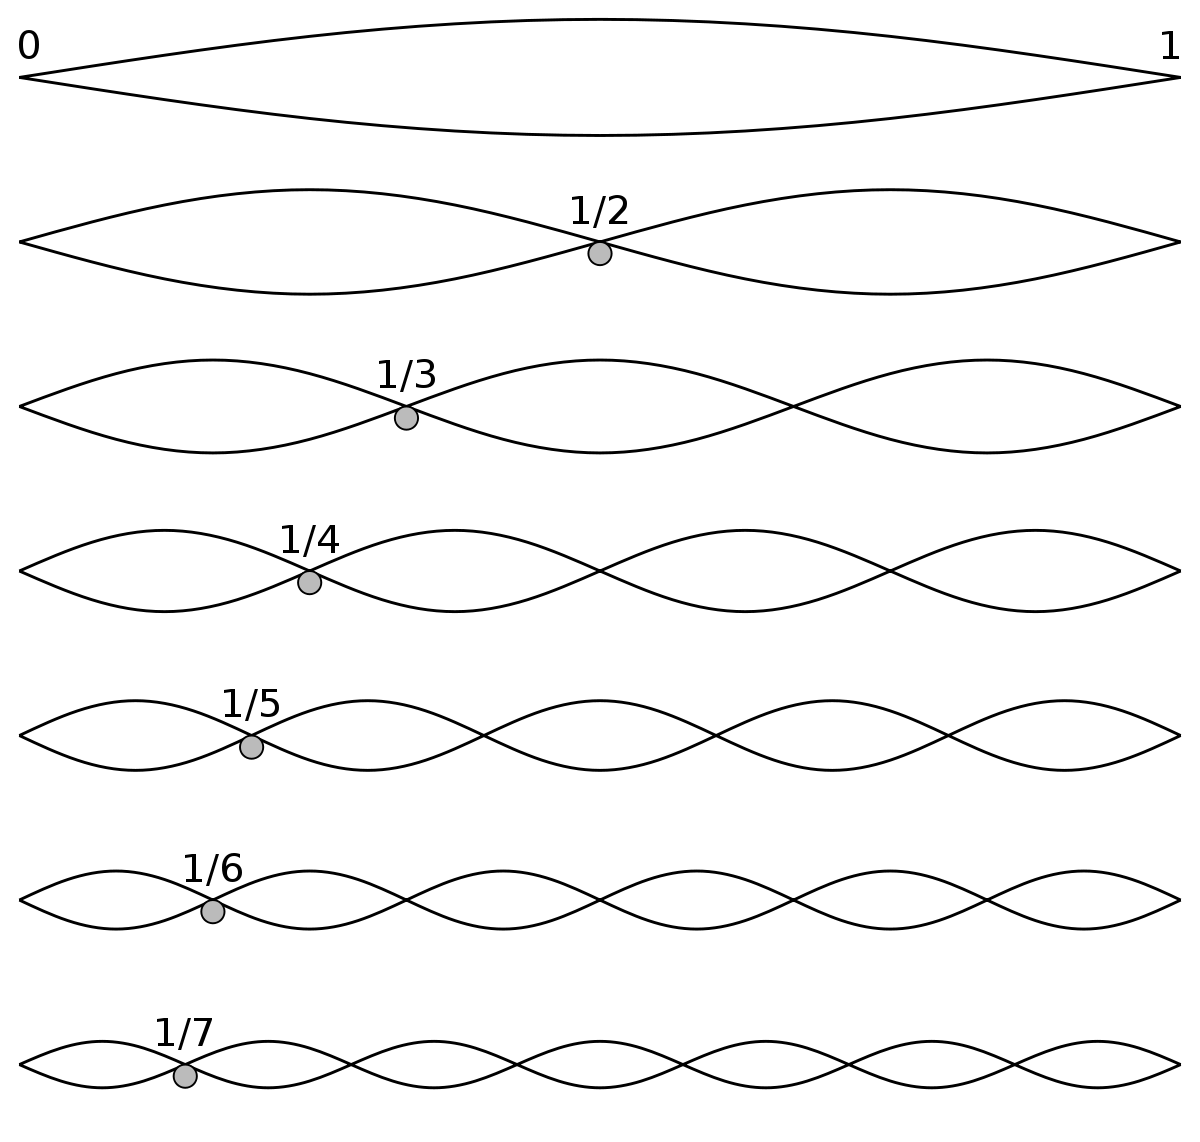
\includegraphics[width=0.5\linewidth]{image/Harmonics.png}
  \caption{A comparison of the wavelengths of waves in a Harmonic Series \autocite{harmonicSeries}}
\end{figure}

\begin{table}[h!]
  \centering
  \resizebox{0.5\textwidth}{!}{%
    \begin{tabular}{|l|l|l|l|l|l|}
      \hline
      \multicolumn{5}{|l|}{\textbf{Harmonic}} & \textbf{12TET Interval}                                                \\ \hline
      1                                       & 2                       & 4 & 8  & 16 & prime (octave)                 \\ \hline
                                              &                         &   &    & 17 & minor second                   \\ \hline
                                              &                         &   & 9  & 18 & major second                   \\ \hline
                                              &                         &   &    & 19 & minor third                    \\ \hline
                                              &                         & 5 & 10 & 20 & major third                    \\ \hline
                                              &                         &   &    & 21 & fourth                         \\ \hline
                                              &                         &   & 11 & 22 & \multirow{2}{*}{tritone}       \\ \cline{1-5}
                                              &                         &   &    & 23 &                                \\ \hline
                                              & 3                       & 6 & 12 & 24 & fifth                          \\ \hline
                                              &                         &   &    & 25 & \multirow{2}{*}{minor sixth}   \\ \cline{1-5}
                                              &                         &   & 13 & 26 &                                \\ \hline
                                              &                         &   &    & 27 & major sixth                    \\ \hline
                                              &                         & 7 & 14 & 28 & \multirow{2}{*}{minor seventh} \\ \cline{1-5}
                                              &                         &   &    & 29 &                                \\ \hline
                                              &                         &   & 15 & 30 & \multirow{2}{*}{major seventh} \\ \cline{1-5}
                                              &                         &   &    & 31 &                                \\ \hline
    \end{tabular}}
  \caption{The relationship between Harmonic and 12TET intervals}
  \label{Tab:harmonic_intervals}
\end{table}

Basically, in a roundabout way, we've affirmed a fairly core and commonly known principle of
melody writing: resolve to the root. However, this is not the only way in which interval patterns
and the Harmonic series are used to determine consonance. Octaves are not actually the only case to
which the Lipps-Meyers law applies. Melodic intervals can be simplified the same was fractions can.\autocite{intervals}
So then, an interval of 9:6, which correlate to the major second and major fifth respectively, could
also be written as 3:2 and therefore follows the Lipps-Meyers law.

Another theory on the relationship between harmonics and dissonance was proposed by physicist
Herman von Helmholtz, who posited that the "beats" created by the resonance of two tones which are
close in frequency can help us quantify the dissonance of an interval.\autocite{intervals} Though it is now regarded
that Helmholtz's theory incompletely addresses the nuances of modern physics and music, it is
a valuable discussion because it provides a foundation from a simplified understanding. Because
of its simplicity, we can more clearly view the connections between harmonics and dissonance and
more easily frame it in a way we might be able to apply with computers which also lack such nuance.
An important part of Helmholtz's theory was that harmonic intervals of smaller integers tend to
create higher degrees of consonance.\autocite{intervals} This much is evident in common chord
structures. For example the major tonic is composed of harmonics 1, 3, and 5. Conversely, the
diminished tonic - commonly viewed as more dissonant - is composed of the harmonics 1, 11, and 19.

\subsubsection{Contour}

Intervals primarily address each note only in relation to the note directly prior; however, melody
is also constructed upon more macroscopic contexts. This is where contour comes into play. Contour
describes the "shape" of a melody by its repetition, conjunctness, and direction of motion.\autocite{contour}

Repetition is straightforward; it describes the reoccurrence of a note or series of notes. Too much
repetition in a melody tends to make it feel monotonous, while too little makes it erratic and
difficult to follow.\autocite{contour}

Conjunct motion is also referred to as step-wise motion because it denotes that each note is within
one diatonic step (a major or minor second interval) of the note prior. Its opposite - disjunct
motion - refers to melodies containing intervals larger than the diatonic step. Disjunct motion can
add a dynamic element to a melody, but when a melody jumps too large an interval in too short a
time span, it not only generates a lot of tension, it also makes the melody more difficult for a
human to play. For both of these reasons, we should aim to keep our AI outputs to a reduced degree
of disjunctness.\autocite{contour}

Direction in a melody refers specifically to vertical direction. A melody is considered to be
ascending when each note has a higher pitch than the previous and descending when each note is of a
lower pitch than the previous. Fluid motion tends to come across more melodically in music. As
such, it is more desirable to maintain the direction of a melody for a certain period of time
before switching it as opposed to having notes rapidly alternate between ascension and descension.\autocite{contour}

\subsection{AI}

The artificial intelligence of this project should be able to generate a melody using
a piece of original melody as input. Ideally, it would be able to extend the input at a
similar length and with similar tonality, mood, tension. For this, we research
a couple of different alternatives, with their own sets of advantages, disadvantages, and
trade-offs.

\subsubsection{First Approach: Computer Vision. PixelCNN}

Our original concept for the AI model took a computer vision approach. To begin we would
have had to develop a script which could convert between MIDI data and a PNG
visualization. This image would be similar in structure to what might show on the piano
roll display of a DAW. Each pixel along the vertical axis would represent a key on the
MIDI controller, and each pixel along the horizontal axis would represent some small
fraction of a beat - hypothetically the length of a sixty-forth note, as this is the
shortest common time interval in music. The hue of each pixel would denote the velocity
of the note being played at that time and pitch - a black pixel would mean no note is
being played while a white pixel would show a note being played at maximum velocity.
These images could then be fed into a Convolutional Neural Network (CNN) which would
replicate the visual patterns and thereby output an image that can be converted back into
a MIDI of a completed melody.

\begin{figure}[h!]
  \centering
  \includegraphics{image/MIDIsample.png}
  \caption{Example of a visualized MIDI file}
  \label{fig:midi_sample}
\end{figure}

This approach was originally considered for its advantages over a more direct MIDI-based
AI. For starters, when conducting some test trials, it was found that the PNG
visualizations are about a quarter the file size of the original MIDIs they were converted
from. This, in conjunction with the comparatively easy calculations of a CNN on a
simplistic bitmap, suggested that a computer vision model would be fast to train.

Additionally, patterns in music are much easier to recognize through visualization than
through note data. Much of the music theory that determines whether a note is melodic in
context is generalized in that it works according to intervals as opposed to discrete
relationships between specific notes. MIDI files don't provide any information about
scales or chords; they simply list which notes were played. It might take an AI a good bit
of to recognize that the interval between C and E is the same as the interval between F
and A - and even longer still to determine which intervals are musically dissonant or not,
and in which contexts. When music is visualized, however, it can generalize the same way
it does in abstract theory. Melodic intervals appear visually the same, regardless of the
root note. So rather than having to learn separately that C pairs well with E and F pairs
well with A, it can generalize that any note will pair well with the note that is four
semitones (or in the AI's case, four pixels) above it, known in music theory as the major
third.

The computer vision model was also favored for its level of technical skill. As students,
we have been exposed to the concept of CNNs but have not yet had the opportunity to apply
them. This model felt appropriate for our skill level because it is centered around a
technique we already understand, but it also implements that technique to a degree we have
never attempted before.

\paragraph{PixelCNN}

For the computer vision model, our lead candidate was PixelCNN. Like a standard CNN,
PixelCNN processes its image inputs primarily through layers of masked convolution.
The "masks" used in the convolution layer are square matrices, and each element of the matrix
is a numerical value that denotes the weight of that element. These masks are iterated over the
input image, convolving with the brightness of the pixels under the mask. In colored images,
the process is repeated once for each color channel: red, green, and blue.\autocite{pixelCNN} Depending on the
configuration of the weights in the matrix, different masks can be used to identify different
visual patterns. Each convolution with each mask outputs a two-dimensional array of values
called a feature map.

Unlike a standard CNN, however, PixelCNN specifically uses masks that only allows it to read
one pixel at a time: row by row, and left to right in each row.\autocite{pixelCNN} This enforces that each pixel
is dependent upon only those above and to the left of itself. Using this unique relationship,
PixelCNN has a unique use-case in predicting the bottom half of an image after processing the
top half as input. The AI uses the probability distribution of visual features found in all pixels
iterated through prior to inform the probability distribution it creates to predict the pixels that
will follow.\autocite{pixelRNN}

\begin{figure}[h!]
  \centering
  \includegraphics{image/PixelMask.png}
  \caption{PixelCNN's unique mask prevents the AI from peeking ahead}
  \label{fig:pixel_mask}
\end{figure}

This made PixelCNN a particularly appropriate candidate for our computer vision model
because completing an image after processing the first half is exactly the mechanic we
planned to use to achieve the melody autofill. All we would have to do is rotate the input
image such that the time axis propagates top to bottom as opposed to left to right.
Additionally, the dependencies that PixelCNN establishes simulate dependencies in music
really well. Whether or not a note is melodic depends on its context - specifically, the
notes that came before it in time as well as the other notes being played at the same
time. Adjusting the axes, PixelCNN's dependency upon all pixels above equates to the
current note being dependent on all notes that were played before it. As for its left to
right dependency, chords are typically built upward from the root - which, when rotated,
would be left to right.

Our main challenge in the use of PixelCNN would be the collection and preprocessing of
training data. For this model to work for our purposes, we would have to convert each MIDI
file into a piano roll visualization which is rotated 90 degrees clockwise.

\subsubsection{Second Approach: Already existent libraries. Magenta.}

Before starting to develop a solution, we checked on existent libraries, researches and
open source projects. This gave us a broader idea about the possible factors that can
become in major challenges. Examples of these factors could be: find and prepare datasets,
choose the correct AI prediction model, and what resources are required for training. We
found that Google AI has released in 2018 an extensive library for art and music
applications: Magenta.

\paragraph{Magenta Project} This collection of libraries is specific for music and art
creation. It contains already trained AI models, different tools for MIDI handling, API
and datasets that can be directly used to solve our problem. Although, the level of
functionalities already included in the main API can defeat the academic purpose of the
current project. Still, some of this elements can be valuable tools to create, train, and
use our own autocomplete AI model. Either way, here we analyze the parts of the library that
can be applied to our project.

\subparagraph{MusicRNN} The module MusicRNN offers a close to ideal solution for the
autocomplete functionality. This module contains models for generating and performing
sections of melodies \autocite{musicRNN}. The models of interest are MelodyRNN, ImprovRNN,
and PerformanceRNN. All these models, as their name implies, are based on recurrent neural
networks (RNN) produced with Google's TensorFlow.

\subparagraph{Recursive Neural Network (RNN)} In contrast with the already mentioned CNN,
that processes grid values without contextual information, RNN processes sequential data
as string of characters, words, or in our case of interest, melody representations. RNN
also considers proccesed information along large sequences of data, and not purely local
extent as CNN.\autocite{fundamentalML}

\paragraph{MelodyRNN.}
MelodyRNN model generates melody based on an input melody. To achieve this, it uses
language modeling (probability distribution over a sequence of data) with long short-term
memory (LMST) networks. This is a variant of RNN design to improve the performance of
regular RNN across large sequences of data. The main issues that LMST address are those
related to the exploding and vanishing gradients magnified on any recursive network due to
the accumulation of errors on the successive feedbacks of data analysis. This models also
have four configurations to assists determining the range of pitches, identifying
recursive patterns, and pay special attention on specific sections of the input melody
\autocite{melodyRNN}. This model alone could be in charge of the autocomplete feature we
are looking to achieve in our project.

\paragraph{ImprovRNN.}
ImprovRNN generate melodies in the same fashion of MelodyRNN. The main difference with the
before model is the conditioning of the generated melody to a chord progression. This
model counts with similar set of configurations than MelodyRNN, but with the addition of
using as inputs vectors representing chords of the progression. Although, this can be a
interesting feature to generate melodies, the model requires to encode the full input
melody in XML format, not supporting direct MIDI input \autocite{improvRNN}.This model
would not be directly applied to our project, but still could add interesting features for
an expanded instance.

\paragraph{PerformanceRNN.}
PerformanceRNN generates melodies using dynamic and expressing timing. This allows to
generate more natural feeling as if a real player is adding to the expression of the
performance. Although, this came with some trade off as some keys can fall outside the
proper timing. \autocite{performanceRNN}

This model add a nice to have feature, but is not fundamental for our first aproach.

\paragraph{Datasets.}
Magenta project offers a set of collections of data that has been used to pre-train
models. From this collection, seems that the MAESTRO (MIDI and Audio Edited for Synchronous
Tracks and Organization) dataset could be the most useful for this project. It contains
over 200 hours of key annotated piano performing. Other set that can be useful for our
classical music approach is the Bach Doodle Set. A large audio dataset (over 6 years of
total audio), collected by Google using its Bach Doodle. \autocite{magentaData}

The selection of the dataset would be conditioned by the available trianing capabilities
for this project.

\subsubsection{Third Approach: Develop out own RNN. LSTM.}

(This is under research by Jorge)


\subsection{Embedded Controller Comparisons}
\label{sec:embedded_controllers}

\subsubsection{Raspberry Pi 4 Model B}

\begin{figure}[h!]
  \centering
  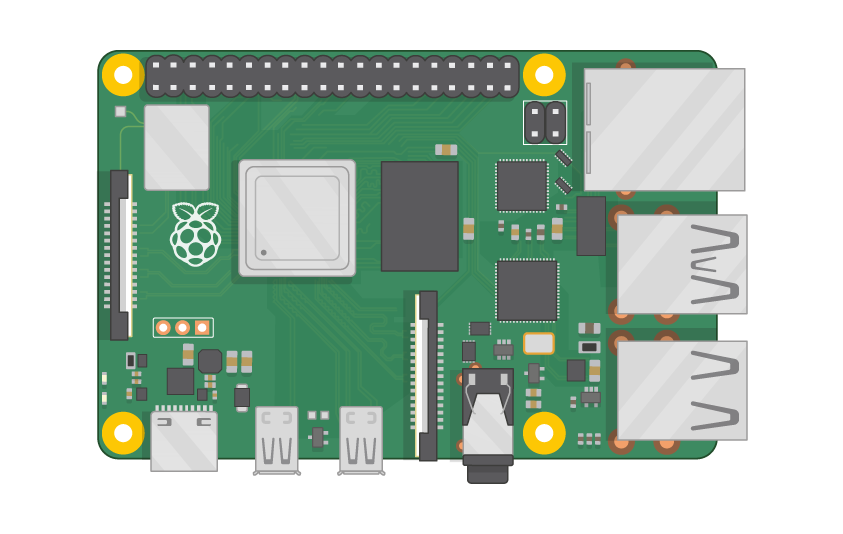
\includegraphics[width=\linewidth]{image/raspberry-pi.png}
  \caption{The Raspberry Pi 4B \autocite{raspberry-pi-4b}}
  \label{fig:rpi4b}
\end{figure}

The Raspberry Pi is a mini-computer which can act as an embedded controller using GPIO
pins. This is an appealing option to us, as it is easy to use and members of our group
have previous experience with it, and one of our members already owning a Raspberry Pi to
test on. What makes the Raspberry Pi more than just a embedded controller is the GPIO pins
that are located in the top of the board as seen in \autoref{fig:rpi4b}. These pins are
designed to allow the Pi to interface with other electronics, such as buttons attached to
our keys. Each pin serve a different purpose, and we will be using a few of them.
Otherwise the Raspberry Pi 4 functions as a normal computer, with the ability to plug in a
keyboard, mouse and monitor. The Raspberry Pi can run any armv7 Linux distro. The
operating system is loaded onto it using an SD card. The Raspberry Pi is typically powered
using USB-C and a power supply, but it can also be powered through one of the GPIO ports,
with a 5V connection. The Raspberry Pi also features an ethernet port and a headphone
jack.

The Raspberry Pi has a baseline cost of \$35 for the 2GB of RAM edition, \$55 for the 4GB
edition, and \$75 for the 8GB edition. We intend to use the 4GB edition, which will meet
our memory requirements for running an electron app and an AI. This price is within our
budget constraints.

The Raspberry Pi can be seen as overkill for many projects, where a cheaper embedded
controller, such as an adruino, could be used instead. Our project is computationally
expensive, so it makes sense for us to use good hardware. Although it may be possible to
do this project with a cheaper embedded controller, it would be risky to design our
prototype with cheaper hardware. We know from preliminary testing that the Raspberry Pi
will provide the computation power and memory our project needs. We prefer to start with
hardware we know will meet our specifications from the start.

\subsubsection{Conclusion}

We have decided to use the Raspberry Pi 4 for our project. We know from our research that
the Raspberry Pi will meet our specifications. Our previous experience with Raspberry Pi
is a big advantage, and working with a full blown Linux environment will save us valuable
development time.


\subsection{DAW Frontend Technologies}

We are looking to use a browser-based frontend Design. This approach is ideal for its ease
of implementing a user interface as well as its cross-platform compatibility. Should we
decide to make the software even more portable by isolating it from the MIDI controller,
it will be viewable on any device that can run a browser. And because of the computational
limits of the MIDI controller, any modern device that is suited for a browser will
inherently be able to run the MIDI autofill software as well.

We experimented with several options for a UI-building environment. Our first consideration was
React. Considering our group's familiarity with JavaScript as well as HTML and similar markup
languages, it would be easier to pick up. Electron offered a similar level of convenience, but with
an added implementation of Node.js that would make our code more modular. Another strong candidate
was Google's Flutter. Flutter's default stylization is sleek and fits in well with the modern
aesthetic of technology. Plus, its widgets allow for more polish on a UI that also has more niche
functionality.

Our frontrunners after all options had been proposed were Electron and Flutter. Utlimately it was
our hardware constraints that pointed us toward Electron because the HTML and JavaScript
application was the most likely to be compatible to run on the Raspberry Pi.

As established in \textbf{\ref{sec:daw} \nameref{sec:daw}}, the primary aspect of the UI
will be the piano roll display. The frontend will be responsible for reading the MIDI
messages and converting the note ON/OFF and timing clock features into the position and
dimensions of an arbitrary number of UI elements - each representing a note which can be
edited.

\subsection{Raspberry Pi}

As mentioned in \textbf{\ref{sec:embedded_controllers} \nameref{sec:embedded_controllers}},
the Raspberry Pi is mini-computer which can also function as an embedded controller. The
model we're interested in is the Raspberry Pi 4B, which is the latest model and has the
best hardware. After an analysis of other solutions, we have decided that the
Raspberry Pi is the best fit for our project. To that end, we have researched how the
Raspberry Pi can be configured for use in our project.

\subsubsection{Operating System Choice}

The first configuration choice that needs to be made is the operating system. A Raspberry
Pi out of the box has no operating system. An image must be flashed to an SD card to make
the Raspberry Pi useful. Raspberry Pi's typically run some form of Linux. The Raspberry Pi
4B model uses the AArch64 architecture. It can run most AArch64 based Linux distros, but
we must limit ourselves to armv7 (32 bit) operating systems, as tensorflow does not
natively support AArch64 as of the time of writing. Tensorflow lite supports AArch64, but
tensorflow-lite has a limited number of supported operations, which can inhibit our
development. There are still many OS choices available, as there are many flavors of Linux
that can run on the armv7 architecture. Some common choices for Raspberry Pi include
Raspberry Pi OS (formerly known as Raspian), Arch Linux ARM, and DietPi. Each OS has its
advantages and drawbacks, and it is important for us to select a distro that is well
suited for our use case. We will need to modify the system heavily for our purposes, but
we need a good baseline for modification.

We need our distro to be a lightweight bootloader for our application. There are many
examples of highly specialized distros designed for one specific task. Examples
include RetroPIE, which is used to run retro video games, or OpenMediaVault, which is used
to turn the device into a networked storage device. This is similar to what we want our
operating system to do. Our use case for the Raspberry Pi is to run one specialized
application that we ourselves develop. It should boot straight into our application with
no other UI from the operating system. The best solution for us is to have a custom distro
just for running our application. Developing a Linux distro from scratch is a difficult
process that is out of the scope of this project. But what we can do is modify an existing
distro to suite our needs. We plan to do this process using a tool called Packer,
described in more detail in Section \ref{sec:packer}.

\paragraph{Raspberry Pi OS}

The most common operating system used for Raspberry Pi is Raspberry Pi OS, which is
developed by the Raspberry Pi Foundation. This is a specially tailored version of Debian
for the Raspberry Pi. This is a common choice for any general purpose usage the Pi. It can
be used like a normal desktop computer when a mouse, keyboard, and monitor are plugged in.
This is a "batteries included" distro that includes things we do not need, such as a
desktop environment, login manager, and various desktop apps. The extra software from this
distro can hinder performance and waste SD card space.

Raspberry Pi Foundation is aware that this distro is too heavy for a lot of Raspberry Pi
projects. To mitigate this issue, they provide lightweight edition known as Raspberry Pi
OS Lite. This version does not include any desktop environment or other extraneous
software. As a result, Raspberry Pi OS Lite fits in 442 MB, which is a big improvement
over Raspberry Pi OS, which is 1175 MB. This makes Raspberry Pi OS Lite a better choice
for our use case, as it would be easier for us to build up to what we need rather than to
cut what we do not need.

\subparagraph{Pros}
\begin{itemize}
  \item Very well documented
  \item Has the best support for Raspberry Pi
\end{itemize}

\subparagraph{Cons}
\begin{itemize}
  \item Comes with unnecessary software
\end{itemize}

\paragraph{DietPI}

DietPi is like Raspberry Pi OS Lite in that it is a lightweight distro. DietPi's claims to
be even lighter than Raspberry Pi OS Lite. It occupies 589 Mb on the SD card, while
Raspberry Pi OS occupies 1424 MB. There are other system optimizations in place to improve
general performance as well. After boot, there are 11 total processes, versus 18 total
processes running on Raspberry Pi OS. This is a good choice for base system. It is easier
for us to start lightweight and add what we need, rather than to start with a bloated
system and strip it down. DietPi comes with a flexible configuration utility that allows
the system to be customized for a specific use case, as show in \autoref{fig:dietpi}.

DietPi includes a configuration menu in the installation for software that runs after
boot. In this menu there is a way to run chromium in kiosk mode. This is an item that we
need to configured anyways, as described in Section \ref{sec:research:subsec:os_config},
which also makes DietPi an appealing choice. DietPi also supports a fully automated
installation process, which we intend to take advantage of, as will save us time from
needing to flash the Raspberry Pi and go through the installation process whenever we
change the operating system configuration.

The main downside to using DietPI over Raspberry PI OS is that there are many tutorials
and documentation for using the Raspberry PI with Raspberry PI OS, that may not apply to
using DietPI, or will be a different process.

\subparagraph{Pros}
\begin{itemize}
  \item Lightweight
  \item Automated installation
  \item Flexible and easy configuration
\end{itemize}

\subparagraph{Cons}
\begin{itemize}
  \item Not as much documentation as Raspberry Pi OS
\end{itemize}

\begin{figure}[h!]
  \centering
  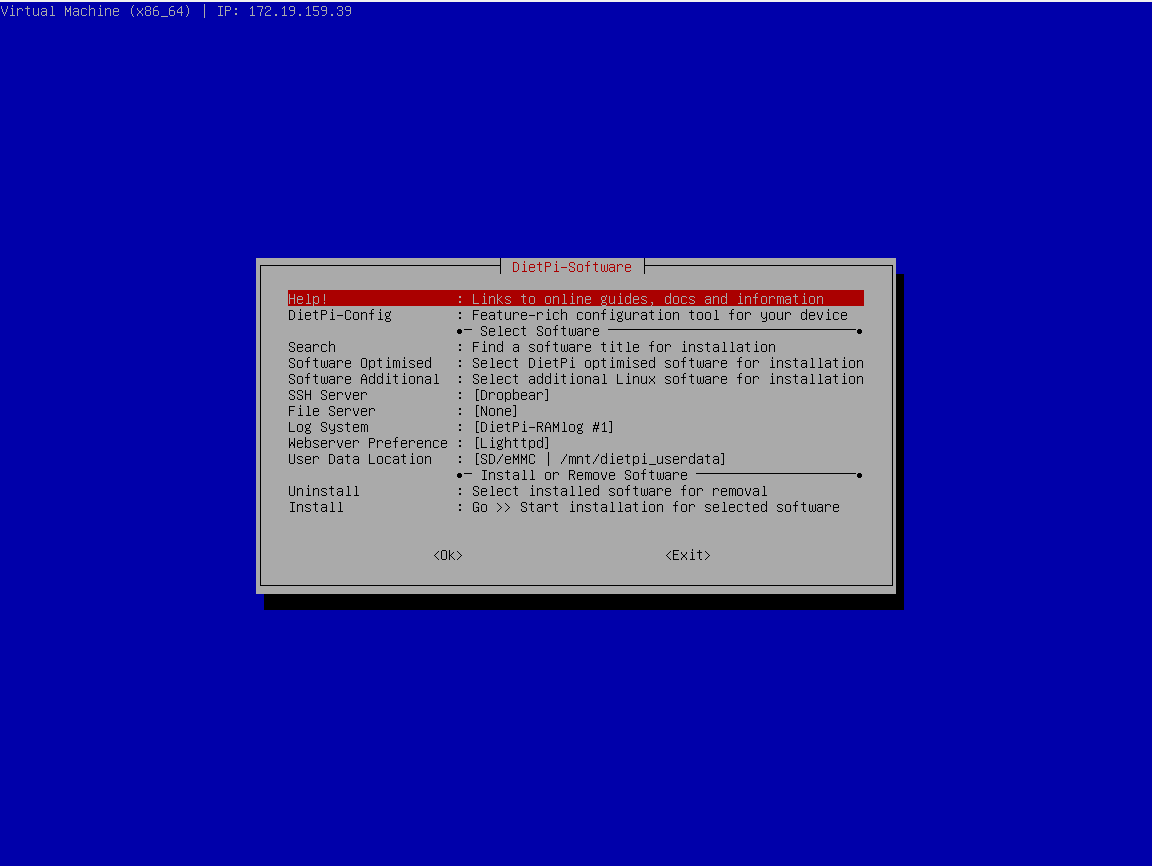
\includegraphics[width=\linewidth]{image/dietpi-config.png}
  \caption{DietPi's Installation Menu}
  \label{fig:dietpi}
\end{figure}

\paragraph{Conclusion}

From our research, we have decided to use DietPi as a baseline operating system for our
project. The lightweight aspect suits us well, as we only need to boot a single
application. The high degree of customization makes it easy to have a minimal system
tailored to our application. The easy chromium kiosk mode configuration is also a big
bonus, as it relieves us from a configuration burden. The installation of DietPi will be
automated using the automated install process, and further customized using Packer.

\subsubsection{Operating System Configuration}
\label{sec:research:subsec:os_config}

The operating system will need to be configured for our use-case. We need to get the
operating system to boot a single GUI application, our DAW, without displaying any other
UI from the desktop environment (DE). There may be more applications separate from the DAW
that will run in the background which also must started immediately after boot such as an
application that acts as the MIDI backend, sending the MIDI notes to the host PC, which
will likely be a separate component from the DAW itself. The operating system will need to
be configured to not permit any networking out of security and privacy concerns.

To only display a single application, we need to configure the graphics system in our
distro. Graphics in Linux are done through the X Window System. In modern apps, X is
mostly agnostic to the UI, and is used for providing UI toolkits a method for accessing
bitmaps to windows. X can be configured in a variety of ways. The way we intend to
configure X is to host a single fullscreen application for our DAW. This can be done
through the \url{.xinitrc} file. This file specifies which commands to run whenever the X
server starts. By including the command to run our application in there, we will have a
single window at startup.

\begin{lstlisting}[language=bash, label={lst:xinitrc}, caption=Example .xinitrc]
#!/bin/sh

exec chromium --kiosk http://127.0.0.1:8080/
\end{lstlisting}

Because our app is browser based, the startup application will be a web browser. In our
case we want to use the Chromium browser, which is the open source variant of Google
Chrome. Chromium has a feature called Kiosk mode, which puts the browser in fullscreen
with no border or frame \autocite{chromiumKioskMode}. This in combination with the xinitrc
file fulfills our requirement of only having a single fullscreen application with no other
UI. This feature can be enabled through the \url{--kiosk} command line flag
\autocite{chromiumKioskMode}. See \nameref{lst:xinitrc} for an example of an xinitrc that
launches chromium in fullscreen mode. DietPi can also handle this configuration for us,
using the \url{dietpi-autostart} configuration utility (See
\autoref{fig:dietpi-autostart}).

\begin{figure}[h!]
  \centering
  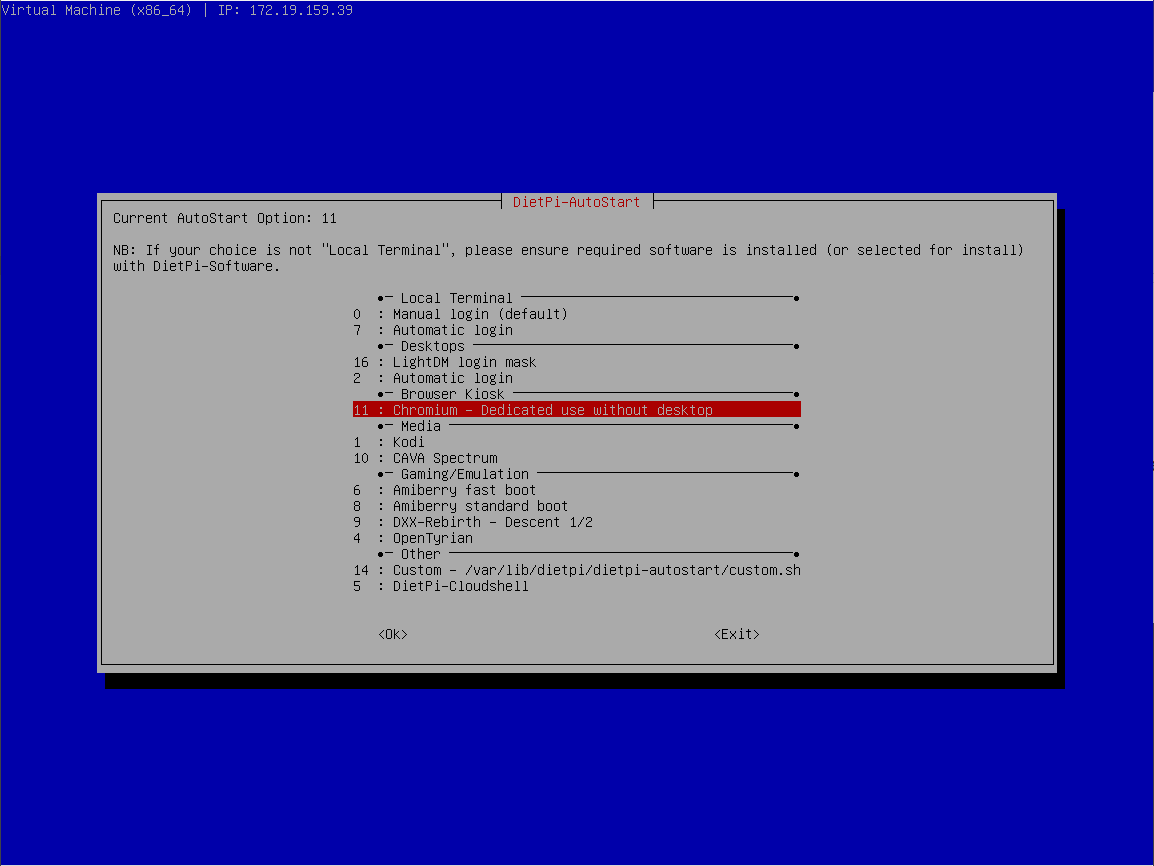
\includegraphics[width=\linewidth]{image/dietpi-autostart.png}
  \caption{DietPi's Autostart Menu with Chromium Kiosk Option}
  \label{fig:dietpi-autostart}
\end{figure}

For the final product, we will want to have networking disabled. We will need network
connectivity while in development, so we can use SSH and LAN, so we need to make sure that
we switch it off for the final rpdouct. Networking can disabled through the
\url{/etc/network/interfaces} config file. This config file is used to declare all
networking interfaces, and the interfaces can be removed by simply removing all lines
declaring a networking interface in that file. We can remove all networking interfaces
except for the loopback (\url{lo}) interface, which is the localhost interface that is
important for the system to function properly.

The MIDI connection is going to happen through MIDI over Bluetooth Low Energy, which will
require operating system configuration. This configuration happens through the BlueZ
stack, which is the Linux component responsible for handling Bluetooth, and will be
configured using the BlueZ utilities and configuration files. This configuration process
is quite extensive and is covered in more detail in \nameref{sec:ble_midi}.

\subsubsection{Packer}
\label{sec:packer}

A solution we found for customizing an existing Linux distro is Packer. Packer is a
utility that can take an existing operating system image, change it, and produce a new
image. Modification is done through provisioners, which exist to perform steps, such as
copying files, running shell commands, setting permissions, etc. Packer relies on builders
to carry out the tasks laid out in a configuration file. The builder we will use is called
packer-builder-arm, which builds ARM images and is suitable for a Raspberry Pi.

Packer is configured through simple JSON files. These JSON files contain information about
the original operating system's image, such as the URL it's hosted on, as well as other
metadata about the image. The JSON file also configures provisioners to modify the
operating system. With this provisioners, we can create our own packer json config file to
setup all the tasks described in \nameref{sec:research:subsec:os_config}.

One of the provisioners we will use is the file provisioner, which copies files from the
build tree over to the operating system. For example, the file provisioner can copy the
\url{.xinitrc} file to the home directory, which configures X11 for our application.
We will also use file provisioners to copy over the \url{/boot/} modifications required to
turn the device into a USB gadget, as described in Section \ref{sec:midi_peripheral}.

We will use shell provisioners to run all the DietPi installation and configuration steps.
This will include automating the options we specify in the \url{dietpi-config} and
\url{dietpi-software} utilities. We will also use shell provisioners to clone our DAW
application and any other backend software we need to run on the device. The software
should be pulled straight from the git repository if available.

The final output is a reliable \url{.img} file built, that can be flashed to an SD card
using a simple image flashing utility, such as balenaEtcher. This image will already have
the operating system fully configured and with our software preinstalled onto it, so there
will be no need to do any setup after the image is flashed.

We are also looking into having this packer build be integrated into our GitHub repo with
GitHub Actions, which will automatically build a new image on every pull request. This
will allow us to ensure that the OS build is working before merging any new code into our
upstream. This should give us the confidence to work on the code without fear that we will
break the Raspberry Pi image builds every time.

\subsubsection{Performance}

Performance is always a concern when dealing with constrained embedded hardware. The
Raspberry Pi fares better than microcontrollers you would find in a typical MIDI
controller, but is still performance constrained. Our device needs to be able to run a
machine learning model and a UI application, both of which are computationally expensive
tasks. This is a critical part of our project, so we have conducted extensive research to
ensure that what we want to do is possible on the Raspberry Pi.

\paragraph{Magenta.}

Magenta serves as a good baseline for measuring performance of music generating AI.
Magenta ships with two machine learning models: MusicRNN and MusicVAE. We have performance
tested both of these in a demo benchmark program we have written on the Raspberry Pi 4B.
We have design the benchmark suites to be modular so that we can benchmark our own
checkpoints or models later in development.

The benchmark program we constructed uses Magenta with JavaScript. We use the Tensorflow
node backend for good CPU performance with Node. The program uses both the MusicRNN and
MusicVAE models, with checkpoints that are hosted are Google's servers. The checkpoints
tested are the \url{basic_rnn}, \url{melody_rnn}, and \url{drum_kit_rnn} checkpoints for
the MusicRNN, and the \url{mel_4bar_small_q2} checkpoint for \url{MusicVAE}. The benchmarks
use a JavaScript benchmarking framework called Benny to run several test cases with
magenta, sampling each one several times and providing statistics such as the min, max,
and mean generation time, as well as the standard deviation.

Our benchmarking program has two benchmarking suites: a generalized one to gauge overall
performance (see \nameref{appendix:magenta_benchmark}) and a linear suite to find out what
factors affect performance the most.

In the generalized suite, the MusicRNN model with the provided pretrained checkpoints has
shown good performance overall when autofilling simple and random melodies, well below the
5-second threshold in general with a few edge cases that exceed 5 seconds. With this
knowledge we know it is feasible to run a music generating AI on the Raspberry Pi 4B. What
we need to know is how much we are able to push the music generating AI before we fall
below our threshold. This is where the linear benchmarks come in.

The linear benchmarks allow us to figure out what constraints we have to limit ourselves
to in order to stay below our 5 second threshold. We based these benchmarks around factors
we speculated would affect the performance the most. For each of these benchmark factors,
we progressively test higher amounts and graph the results for easy analysis (see
\autoref{fig:magentaperf}).

\paragraph{Linear benchmark factors}
\begin{itemize}
  \item \textbf{Melody duration.} This is the duration of the input melody in seconds.
  \item \textbf{Number of notes.} Total number of notes in the input melody. This is with
        a constant duration of 16 seconds.
  \item \textbf{Generation steps.} Each generation step represents a quarter note in these
        benchmarks. The duration is constant at 16 seconds.
  \item \textbf{Temperature} This is the temperature of the RNN, which affects the
        randomness of the generated melodies.
\end{itemize}

All benchmarks in the linear suite use random notes quantized to quarter steps. The random
notes fit the checkpoints supported note rage, which is different between checkpoints. For
example, the \url{basic_rnn} checkpoint supports pitches in the range \url{[48, 84]},
while \url{melody_rnn} supports the full MIDI range of \url{[0, 127]}
\autocite{modelPitchRange}.

With this data collected, it becomes easy to analyze what constraints we are working
with. Our target is to remain below 5 seconds of generation time, so we need to ensure
that we have a safe margin below where the graphs meet 5 seconds. The generation time
increases linearly with melody duration and total generation steps. The \url{basic_rnn}
and \url{melody_rnn} checkpoints were neck and neck in terms of generation time, while the
\url{drum_kit_rnn} checkpoint was consistently slower. The temperature had no effect on
the generation time. We were initially surprised to see that the total number of notes had
no effect on generation time, which remained constant when increasing from 100 to 2000
input notes, but this makes sense as the input tensor size does not change with the number
of notes.

The input duration is the biggest factor affecting generation time. The number of
generation steps are the next biggest factor. With this data, we know that we will most
likely need to truncate the input melody's duration to less than 40 seconds of music. The
generation steps need to be accounted for when determining the duration of music to accept
as input for our AI. As the generation steps increase we need make up for that amount of
extra time by decreasing the input duration even further. We added in a benchmark for
increasing duration and generation steps simultaneously to see if this would lead to
exponential behavior, but found that it remained linear. So we can simply subtract the
estimated added time from the input melody duration.

With these benchmark results, we are confident that the Raspberry Pi 4B is capable of
handling the computational load that this project requires, without the need for any
external processing. We also have a good benchmarking solution that can be adapted for any
checkpoints or models that we will further into the project's development.

\begin{figure}
  \centerline{ 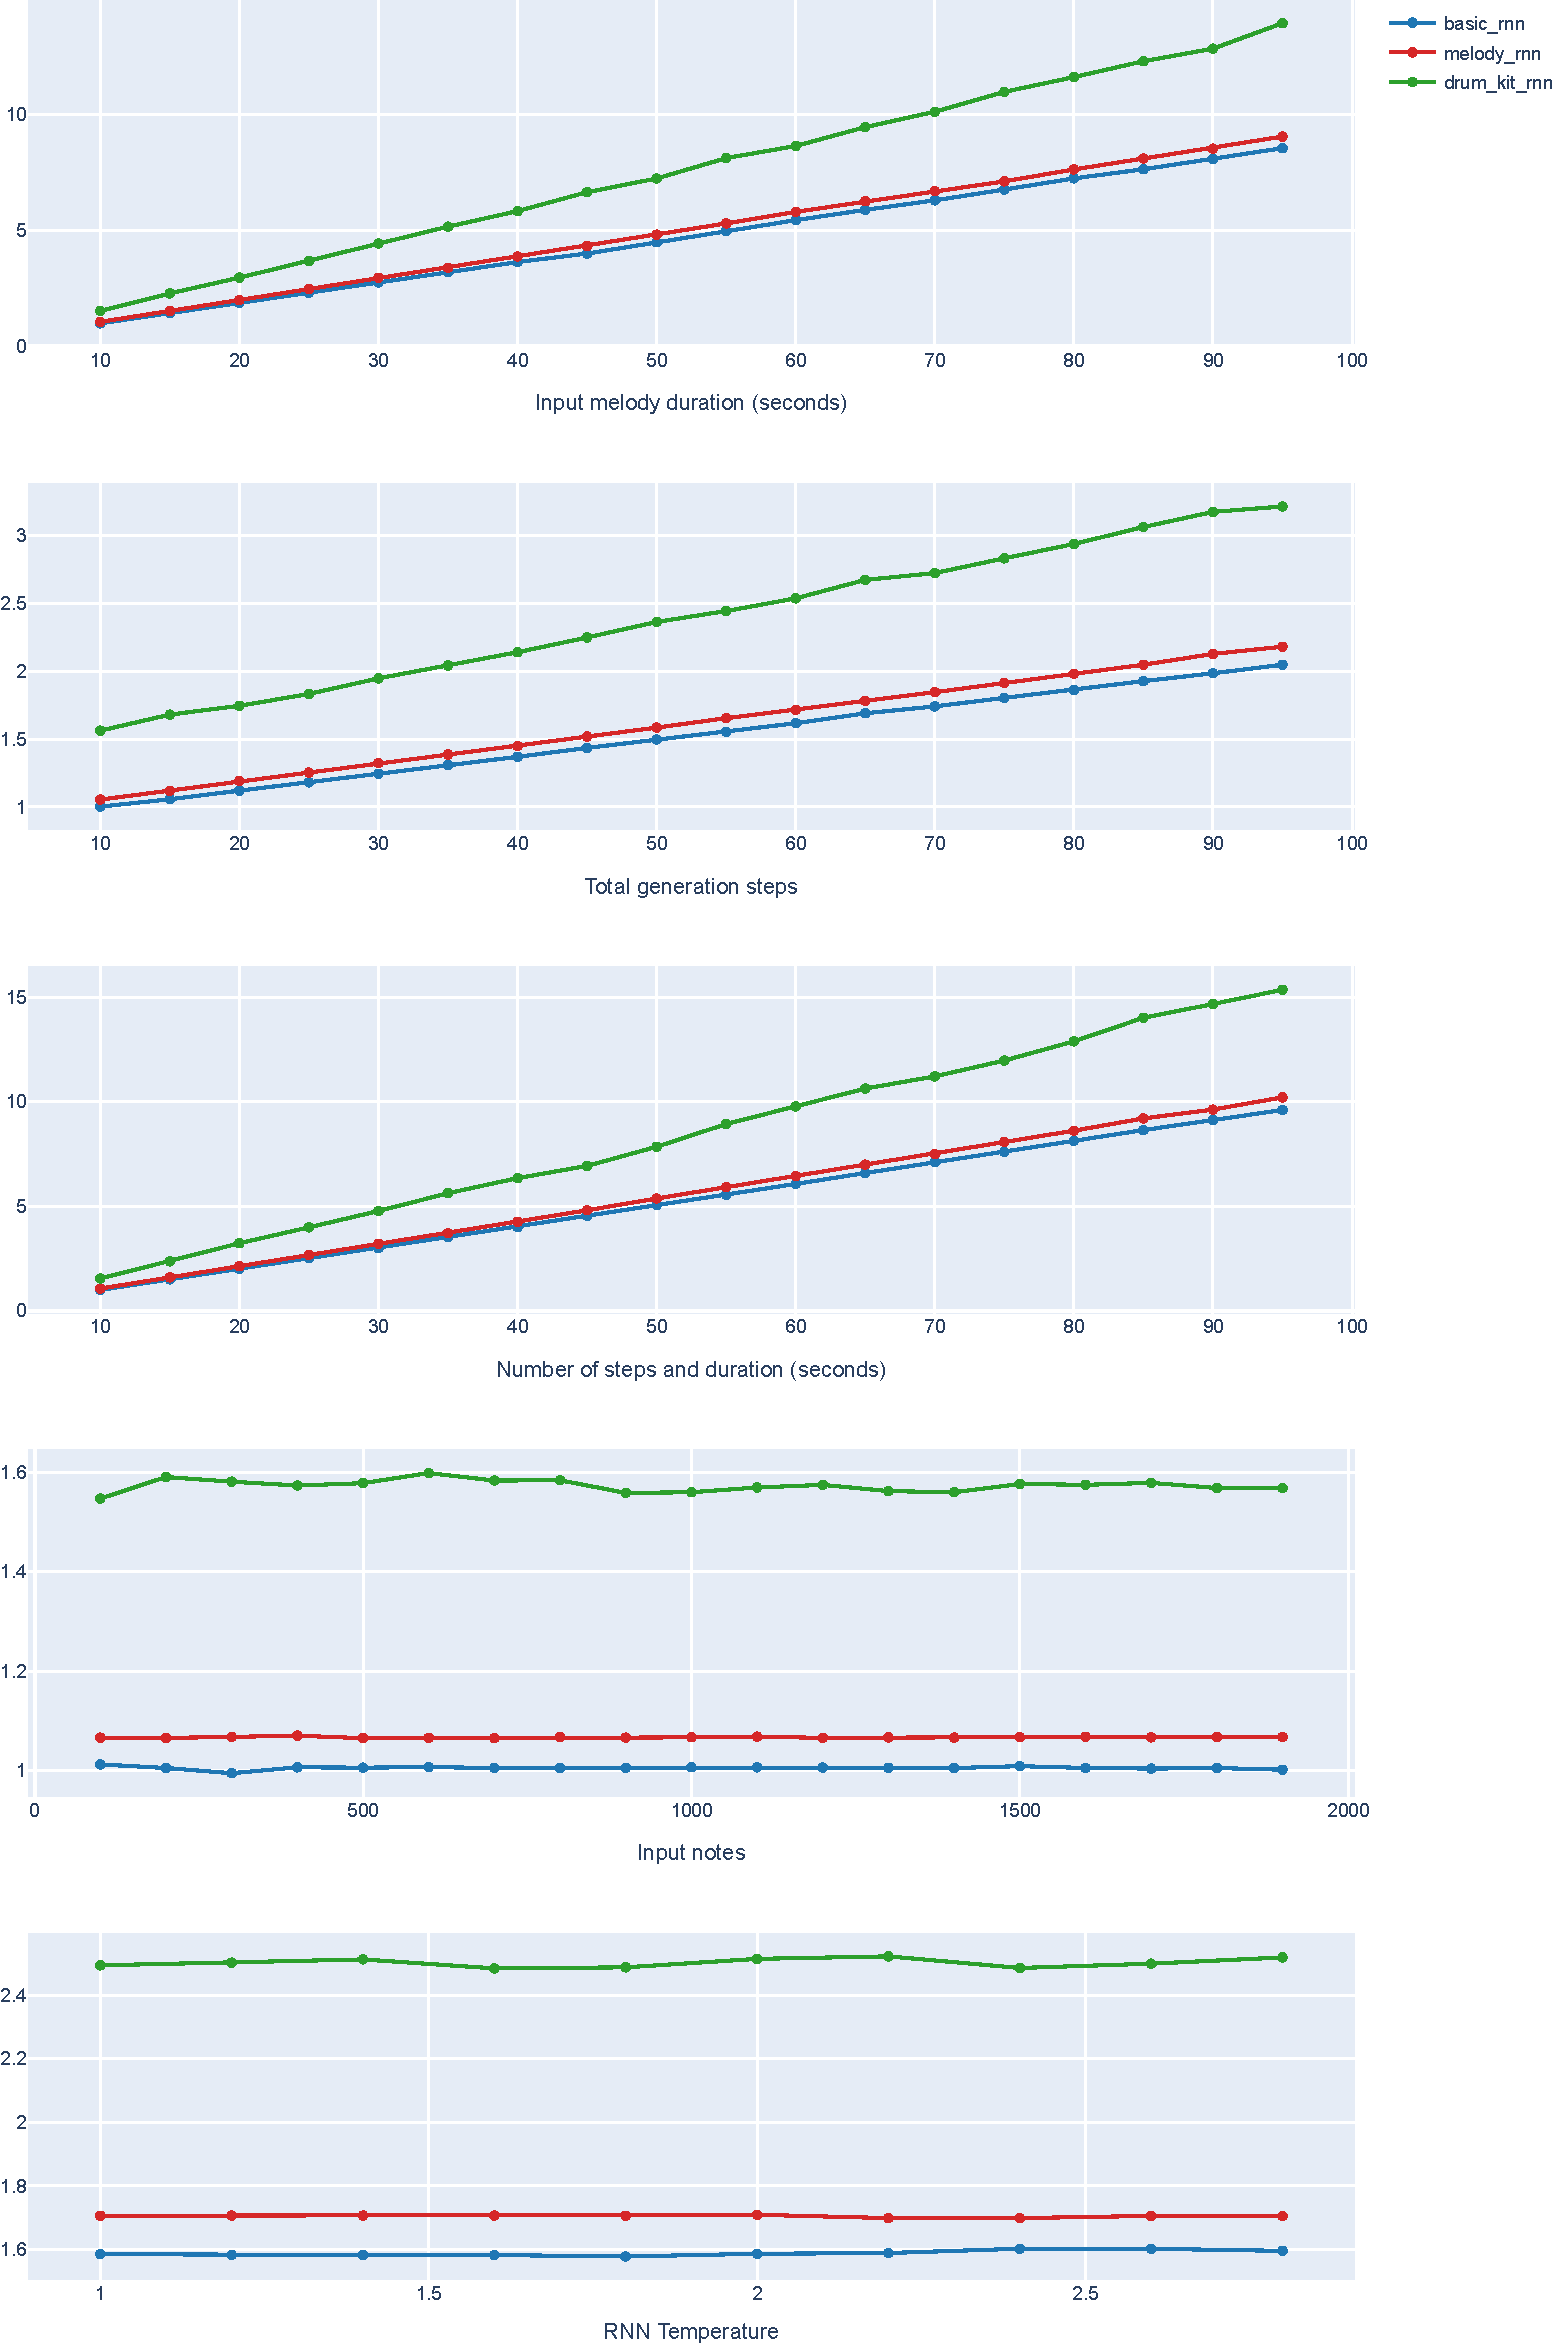
\includegraphics[width=.95\linewidth]{image/perf.pdf} }
  \caption{Magenta Generation Time on the Raspberry Pi 4B}
  \label{fig:magentaperf}
\end{figure}

\paragraph{UI.} It is important to verify that a Raspberry Pi can even run a browser based
DAW with acceptable performance before spending development time creating the web app.
Since we have not developed the DAW at this point, we have tested an existing web based
MIDI editor in the Raspberry Pi.

We used an online MIDI editor called signal (\url{https://signal.vercel.app/}) to get a
subjective feel for the performance. The test was ran in the chromium web browser on
Raspberry Pi OS. The performance was acceptable, with some actions feeling slow.
Dragging around notes had a small but noticeable latency between the mouse cursor's
movement and the notes position. There was also a small but noticeable latency between
double clicking to insert a note and the note showing up on screen. The playhead updated
smoothly when playing the MIDI track, which is the most important aspect, as laggy
playback is awful for the user experience.

It should be noted that this app was not explicitly designed to run on constrained
hardware. Web apps can run great on Raspberry Pis when optimized to do so. Based on our
findings here we are confident that we can develop a browser based app that has
exceptional performance on the Raspberry Pi.

\subsection{MIDI Peripheral}
\label{sec:midi_peripheral}

The Pi needs to function as a MIDI peripheral, i.e. connect the device into a computer and
it functions as a device that sends MIDI commands to the DAW. There are a few different
ways to approach this connection, and we have explored a few such approaches for this
project.


\subsubsection{USB-C Connection}

Under this approach, the connection will happen through a USB-C to USB-A cable from the
Raspberry Pi to the computer. The Raspberry Pi is typically powered from the USB-C port
form a power supply connected to a power outlet, but in our case the Pi will receive its
power from the host PC over USB-C instead. Once plugged in, the Pi will act as a normal
MIDI peripheral, which sends MIDI events to the PC, which can be picked up by a fully
fledged DAW.

The MIDI communication happens over USB in our case, which means we need to work with the
operating system to send these messages. We are using Linux for our device's operating
system, so USB communication needs to happen through the Linux kernel. This is known as a
USB Gadget in the Linux kernel \autocite{usbGadgetDocumentation}. The Raspberry Pi 4b can
act as a Linux USB Gadget through a USB-C to USB-A connection to the computer, with USB-C
being on the Raspberry Pi and USB-A being on the host computer
\autocite{raspberryPiGadgetSetup}. This will not work out of the box, as the Linux kernel
needs to be made aware that we intend to use the device as a USB gadget. This
configuration happens through files in the \url{/boot/} directory
(see listings \ref{lst:bootconfig} and
\ref{lst:bootcmdline}) \autocite{raspberryPiGadgetSetup}. The Pi will act as a USB
gadget after Linux boot configuration settings are set and it is plugged up to the host
machine.

\begin{minipage}{\linewidth}

  \begin{lstlisting}[language=bash,
  label={lst:bootconfig},
  caption=Lines added to /boot/config.txt \autocite{raspberryPiGadgetSetup, raspberryPiHDMIFix}]
dtoverlay=dwc2
hdmi_force_hotplug=1
hdmi_group=2
hdmi_mode=87
hdmi_cvt=800 480 60 6 0 0 0
hdmi_drive=1
  \end{lstlisting}

  \begin{lstlisting}[language=bash, label={lst:bootcmdline}, caption=DietPi /boot/cmdline.txt modified to allow a USB Gadget \autocite{raspberryPiGadgetSetup}, breaklines=true]
console=ttyS0,115200 console=tty1 root=PARTUUID=8f4dbd00-02 rootfstype=ext4 elevator=deadline fsck.repair=yes rootwait quiet net.ifnames=0 modules-load=dwc2,g_ether
  \end{lstlisting}

  \begin{lstlisting}[label={lst:usb_gadget}, caption=Bash procedure to setup a MIDI Gadget\, modified for our device \autocite{raspberryPiGadgetSetup}, breaklines=true]
cd /sys/kernel/config/usb_gadget/
mkdir -p midi_over_usb
cd midi_over_usb
echo 0x17e8  > idVendor
echo 0xb09c > idProduct
echo 0x0100 > bcdDevice
echo 0x0200 > bcdUSB
mkdir -p strings/0x409
echo "fedcba9876543210" > strings/0x409/serialnumber
echo "MIDI Autofill Group" > strings/0x409/manufacturer
echo "MIDI Autofill Device" > strings/0x409/product
  \end{lstlisting}

\end{minipage}

After the boot configuration options are set, the device will be a USB gadget, but there
is more configuration needed for it to act as a MIDI USB gadget. The Linux kernel already
provides an interface for USB gadgets to act as MIDI devices, through the
\url{usb_f_midi.ko} kernel module \autocite{usbGadgetDocumentation}. We need to set our
Raspberry Pi's USB gadget settings to identify itself as a MIDI peripheral. We have
followed an online guide to setup this MIDI gadget, which involves providing information
to the kernel about our device through the \url{/sys/kernel/config/usb_gadget/} folder
\autocite{raspberryPiGadgetSetup}.

From here we can use the \url{aplaymidi} command to test our MIDI device, which sends a
MIDI file to the host computer \autocite{gadgetTesting}. If the gadget is working
properly, then the MIDI sequences should be visible in any application that listens for
MIDI note events, such as a DAW.

USB Gadgets appear as USB ethernet devices and can be read and written to like any other
networking interface. USB MIDI gadgets similarly communicate through standard networking
interfaces under Linux, meaning that our backend program for sending MIDI events to the
host computer will be sending messages through networking interfaces. However, we will
most likely use a library to abstract away this networking aspect.

USB gadgets work, but we ran into a problem with our setup where our HDMI connection to
the monitor was not working anymore. This connection is critical, as we need to be able to
display our DAW to the built in connection using HDMI, so we had to find a workaround for
this issue. We found out that there are \url{/boot/config.txt} options that can added to
force an HDMI connection, using the \url{hdmi_force_hotplug} option
\autocite{raspberryPiHDMIFix}. This configuration as well as some other HDMI settings can
be seen in listing \ref{lst:bootconfig}.

We have also run into some low voltage warnings when running the Raspberry Pi 4B as a USB
gadget. These warnings are found in system logs and are viewed with \url{journalctl}. The
Raspberry Pi 4b requires 5.1 volts and 3 amps to operate effectively, and will send the
undervolt warning whenever it runs below 4.63 volts \autocite{raspberryPiAmps}. We notice
that we see these warnings early in the boot, but it seems to stabilize later. We have not
run into any issues with these undervolts as of now. The Pi does not encounter anymore
voltage warnings when running a CPU stress test, but it could lead to stability issues
later.

This approach runs into a wall when considering how to allow the device to function as a
standalone device, while also being able to receive power through the USB-C connection.
USB gadgets are supposed to be powered through the USB-C port, but when not connected, the
USB device will operate off of a battery. The standalone operation requirement makes this
connection mode very difficult. There is another interface for powering the raspberry PI,
which is the 5 volt GPIO pin. This could be connected to a battery. But then there is the
question of if the Pi can be simultaneously powered by the 5 volt GPIO port while also
being plugged in with USB-C. This may be possible, but there are no resources online that
show how this can be done. It is not worth the time to figure out how this can be done.

\paragraph{Pros}

\begin{itemize}
  \item Lowest latency
  \item Simplest setup, only requiring the end-user to plug in the device
\end{itemize}

\paragraph{Cons}

\begin{itemize}
  \item Wired
  \item Implementation is too complex
\end{itemize}

\subsubsection{RTP-MIDI Over WIFI}

RTP-MIDI is an open source protocol to send and recieve MIDI messages over standard
networking interfaces. RTP-MIDI is built over Real-time Transport Protocol (RTP), which is
a protocol for real-time communication over the network. RTP typically works through UDP
messages over IP. RTP-MIDI can be used over a LAN network. When used over WIFI, the MIDI
device can be connected to another computer without a wired connection. This wireless
factor is convenient for the end user.

With wireless connections, there is always a question of if it can achieve acceptable
latencies. RTP-MIDI over WIFI is fast, and latency is not a major concern. RTP-MIDI Over
WIFI has a latency of around 8.5 ms with a standard deviation of 8 ms
\autocite{ble-latency}.

A major disadvantage of RTP-MIDI is that it is not supported out of the box in Windows 10.
Since RTP-MIDI are just simple UDP network messages, this can be worked around by
downloading a driver, or by using a standalone piece of software. Requiring the user to
download extra software to the computer will degrade the user experience. We want the user
to be able to use the MIDI device with minimal extra setup, and this would hamper that
experience. Addtionally, the user would need to know the IP address of the device on the
LAN, and enter it into the software. This is another step that will hamper the out of box
experience. This can be avoided if the user is running the Bonjour service, but that is
another step that could potentially cause problems.

This approach would be the easiest to implement from a developer perspective. These are
just simple network messages, without the need to go through any special interfaces. There
is a NodeJS library called \url{node-rtpmidi} which would make RTP-MIDI trivial to
implement on the Raspberry Pi. It would be a matter of simply making the connection and
using the library to send MIDI messages.

\paragraph{Pros}

\begin{itemize}
  \item Wireless
  \item Simplest implementation
  \item Lower latency than the Bluetooth solution
\end{itemize}

\paragraph{Cons}

\begin{itemize}
  \item Higher latency than USB
  \item Requires the user to download additional software
  \item Most difficult for the end-user to setup
\end{itemize}

\subsubsection{MIDI Over Bluetooth Low Energy}
\label{sec:ble_midi}

Bluetooth Low Energy (BLE) is a wireless technology standard that enables BLE compatible
devices to communicate with one another. Despite the namesake, BLE is separate from
classic Bluetooth, intended to consume less power, and is not backwards compatible with
classic Bluetooth. Common examples of BLE devices include BLE speakers, keyboards and
mice. The Raspberry Pi 4B supports BLE, which means that the Raspberry Pi can act as a BLE
device. Using BLE has the benefit of being convenient for the end-user as well, with the
ability to move the device freely and without needing to manage another cable.

Most computers also support BLE, or can be made to support BLE through the use of a
Bluetooth USB Dongle. While BLE is not as prevalent as USB, compatibility should not be a
concern for the majority of devices. Bluetooth is also easy for the end-user to setup,
only requiring the end-user to connect to the device through the operating system's
interface.

BLE can be used for a wide variety of devices. BLE devices communicate through profiles,
which specify the BLE  application and the communication specifications. There is a long
list of standardized BLE profiles, with one such profile being BLE MIDI. While support for
BLE is very common, support for certain BLE profiles is not, as its up to each BLE
implementor to support whatever profiles are needed by the device. However, BLE MIDI is
supported by Windows 10, MacOS, Linux, iOS, and Android \autocite{ble-latency}. With BLE
MIDI being supported by every major operating system, we are confident that we will not
run into any compatibility issues with this approach, except for on older computers.

We initially thought that using BLE would incur too much input latency to be practical for
musicians. Using Bluetooth audio is notorious for its latency. But the latency situation
with BLE MIDI is much better than Bluetooth audio. BLE MIDI has higher latency than USB
MIDI, but the numbers are acceptable. BLE MIDI events have a delay of approximately 12
milliseconds one-way and 26ms round-trip time \autocite{ble-latency}. We find this
latency number to be acceptable for our project.

The Raspberry Pi runs Linux, which means that it needs to work through the BlueZ stack in
order to function as a BLE device. BlueZ is a component of Linux that implements Bluetooth
and BLE. The BlueZ stack supports MIDI over BLE, and in combination with ALSA, it is
possible to turn a Raspberry Pi into a BLE MIDI device.

Audio under Linux is handled through the ALSA interface. ALSA also provides what are known
as sequencer ports, which are used to send MIDI events through an interface that can be
connected to a variety of targets. In combination with BlueZ, we can create an ALSA
sequencer port to send MIDI events over BLE. BlueZ provides a binary called
\url{bt-midi-server}, which creates an ALSA sequencer port that is connected to a BLE MIDI
output. From there, we can send MIDI events over BLE by simply using the ALSA APIs for
sequencer ports. When \url{bt-midi-server} is started, any MIDI Bluetooth connections will
automatically get connected to an ALSA sequencer port. This is a nice abstraction which
allows us to write MIDI code without needing to consider Bluetooth in the code itself. The
\url{bt-midi-server} can be run at startup using a systemd service. Our code will simply
need to check for the existence of the sequencer port to see if we're connected to
Bluetooth.

ALSA sequences are programmed using a C API. This C API can be called from JavaScript
using the Foreign Function Interface (FFI). In this API, clients send sequencer events
through the port, which can encode various MIDI events, such as note on/off, with data
such as the pitch and velocity. This API is simple to use, and will be easy to integrate
into our application.

With this interface, it is easy to create a program that creates a ALSA connection to the
BLE MIDI sequencer port, listens for the keypresses from GPIO events, interprets those
GPIO events, and sends the corresponding MIDI commands to the ALSA sequencer port. The BLE
connection is abstracted away in this configuration, allowing us to just focus on writing
MIDI code.

\paragraph{Pros}

\begin{itemize}
  \item Wireless
  \item Widely supported by all operating systems
  \item Simple implementation
\end{itemize}

\paragraph{Cons}

\begin{itemize}
  \item Highest latency
  \item Extra connection step required from the end-user
\end{itemize}

\subsubsection{Conclusion}

We have decided to go with the MIDI over Bluetooth Low Energy approach. This approach does
to suffer from the same problems the USB-C approach has, and provides an added convenience
factor, allowing the user to use the device without wires. It is also easier for the
end-user to configure, with the end-user only needing to connect to a Bluetooth device
through the operating system's Bluetooth interface. The latency is higher than USB-C, but
it is within our specifications. The implementation is also simpler than using USB-C.

\subsection{Application Architecture}
\label{sec:app_architecture}

Our application will be composed of components that will need to interact with each other.
These components are the UI, music generator, and the MIDI device interface. These
components individually are more suited to be programmed in different languages and
environments, which makes it important to consider how these components should be
designed. There are a few different approaches to the application architecture that have
their own pros and cons. The possibilities we have considered are monolithic application,
a multi-process approach, and a library approach.

\subsubsection{Monolithic Architecture}

This is the simplest approach with a single program handles all aspects of the
application. This single application will display the DAW UI, generate the notes, and act
as the MIDI device interface. Everything would be a single project, and there would not be
a need for any inter-process communication (IPC).

The main advantage here is architectural simplicity. Having separate components makes the
project harder for developers to grasp. Generally, it is easiest to develop a single
application where feasible.

Another advantage is simpler maintenance. With a multi-process approach, when one
component changes, often it is necessary to update other components to work with these
changes.

The main problem with this approach is that some of the components are done better in
other languages and with different environments. For our UI, we are going for a web-based
approach, which would mean using a NodeJS stack. We can generate the notes using
JavaScript as well, as there is Tensorflow for JavaScript. But tensorflow is mainly
intended to be used with python, and there is an ecosystem of AI tools and documentation
we will miss out on when using JavaScript, which will make the implementation more
difficult than python. Futhermore acting as a MIDI device is a low-level process that is
best implemented with a low-level language such as C. Like before, in this instance its
possible to be done in a NodeJS ecosystem, but not ideally.

\paragraph{Pros}

\begin{itemize}
  \item Architecturally simple
  \item No need to implement IPC
  \item Ease of deployment
\end{itemize}

\paragraph{Cons}

\begin{itemize}
  \item Difficulty implementing certain components
  \item Errors affect the whole application
  \item Easy to create highly coupled designs
\end{itemize}

\subsubsection{Multi-process Architecture}

In a multi-process architecture, each major component will run in its own executable, and
communicate using an IPC mechanism. Each component can be developed in an ideal ecosystem,
with the UI being a web-based JavaScript application, the music generator being a python
component, and the MIDI device interface being a low-level C component.

Since these components are not in a single executable, they all need to run concurrently,
which means there will need to be a mechanism that spawns all processes. There are a
number of ways to spawn all these processes, such as using system services, or having a
main process that spawns all the child processes and negotiates the IPC mechanism to all
children. For simplicity, here we are mainly considering the main process approach.

An essential part of this is the IPC mechanism, and there many ways to handle IPC. One
mechanism is to start TCP server over localhost. Components can know where to communicate
based off the port number. This communication mechanism allows for any format of
communication in the body, such as JSON. There are two downsides to this IPC approach. The
first downside is the overhead of having to go through the networking systems of the
operating system. The second downside is the potential of port conflicts, if another
application wants to use a port we designate, but this should not be a problem for our
case as our operating system configuration is tailored to our application. Another
approach we consider is to use Unix domain sockets, which works over networking interfaces
(sockets), but works over a file instead of ports. This approach has less overhead and
doesn't have a port conflict issue. The downside here is more implementation complexity,
as there are less libraries and resources for communicating over domain sockets instead of
TCP. If we intended to go with this architecture, this is the IPC mechanism we would
choose.

The IPC mechanism will require additional code, which will slow development time and
create another maintenance hassle. Not only will there need to be code for using Unix
domain sockets, but there will also need to be code to parse and interpret the messages.
The message format will need to be designed and standardized between the applications, and
if any messages need to change, those changes will need to be reflected in all the
components. For example, if JSON is used for the messages, then any time a field changes,
or another field is added, components that use that message will need to be updated to
interpret the new data structure. Parsing JSON is trivial in python and JSON using third
party dependencies, but doing so in C, which the MIDI interface component would be
programmed in, would be difficult, even with third party libraries. Even in python and
JavaScript, which parse JSON trivially, there is still work to agree on a format.

As mentioned earlier, the main advantage to this approach is to be able to create
components in their ideal language and environments. This is a big advantage for the AI in
particular, as python is the most common choice to develop machine learning AI in, and
there are more libraries, documentation, and tutorials to develop machine learning
applications in python.

\begin{figure}[h!]
  \centering
  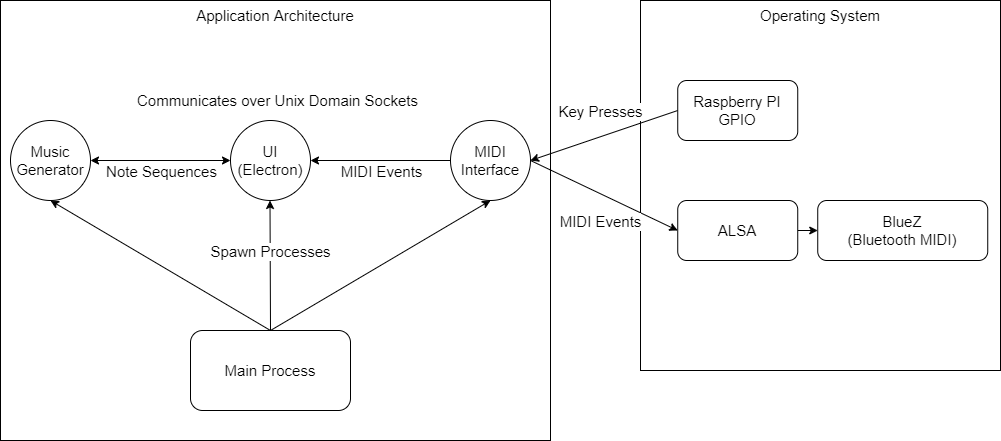
\includegraphics[width=\linewidth]{image/multiprocess.png}
  \caption{Proposed Multi-process Architecture}
  \label{fig:multiprocess}
\end{figure}

\paragraph{Pros}

\begin{itemize}
  \item Ideal language and environment for all components
  \item Loosely coupled design
\end{itemize}

\paragraph{Cons}

\begin{itemize}
  \item Architectural complexity
  \item Need to implement IPC
  \item Need to manage child processes
  \item Need to create a messaging format and parse that format in all processes
\end{itemize}

\subsubsection{Library Approach}

In this approach, there is a main executable supplemented by libraries. The main process
will be a NodeJS based web application and it would libraries for the Music Generation and
MIDI device interface will be handled by external libraries. This would allow the
components to be developed in different languages and environments without the need to
implement IPC and child process management. This approach seemed ideal initially, but
there are some caveats that make this infeasible. Creating a library requires the
developer to create bindings to the libraries. Different languages have different binary
interfaces. The Application binary interfaces (ABI) defines how functions and data
structures are laid out in memory. Bindings are used to bridge the differences between the
ABIs of both languages to allow a library written in one language to be used in another
language.

For the MIDI device interface, which will be programmed in C, this approach works well.
Both JavaScript and Python can call C code through a foreign function interface (FFI). C
has the closest to what can be considered a standard ABI, with the SystemV ABI being a
standard in Linux, with all binaries being in the standard Executable and Linkable Format
(ELF) format. Using the \url{node-ffi} library in NodeJS, the main JavaScript process can
easily integrate with a C library. It is not as straightforward as using a normal
JavaScript library, but it does not take much effort. Python can also interface with C
libraries through its built in CFFI module, but that will not be necessary for this
project.

Where this approach falls apart is creating a binding to python for the music generation
component. Python is an interpreted language, meaning that it is evaluated at runtime
rather than precompiled to a binary. To use python in another language, rather than using
a traditional library, python must be embedded into other languages. Embedding allows a
program written in another language to have parts implemented in a scripting langauge.
Python provides a C library for embedding python code. This is commonly used in games, for
example, where the bulk of the game is implemented in C++ and then simpler tasks are
implemented in a high-level language such as Python for developer productivity. This would
work, but would be tedious in a C or C++ application. In our case, we would need it to be
embedded in a NodeJS application, which is even more tedious. There is a Node library
called \url{pynode} to assist in this process, but it would still cost too much
development time.

\paragraph{Pros}

\begin{itemize}
  \item Ideal language and environment for all components
  \item Loosely coupled design
  \item No need to implement IPC
  \item No need to implement child processes
\end{itemize}

\paragraph{Cons}

\begin{itemize}
  \item Need to implement FFI code
  \item Need to implement code to embed python in Node, which is not straightforward
\end{itemize}

\begin{minipage}{\linewidth}

  \begin{lstlisting}[language=JavaScript, label={lst:node_ffi}, caption=Example of using \url{node-ffi} to call a C library \autocite{node-ffi}, breaklines=true]
var ffi = require('ffi');

var libm = ffi.Library('libm', {
  'ceil': [ 'double', [ 'double' ] ]
});
libm.ceil(1.5); // 2

// You can also access just functions in the current process by passing a null
var current = ffi.Library(null, {
  'atoi': [ 'int', [ 'string' ] ]
});
current.atoi('1234'); // 1234
\end{lstlisting}

\end{minipage}

\begin{minipage}{\linewidth}

  \begin{lstlisting}[language=Python, label={lst:pynode}, caption=Example of using \url{pynode} to embed python in JavaScript \autocite{pynode}, breaklines=true]
const pynode = require('@fridgerator/pynode')

// Workaround for linking issue in linux:
// https://bugs.python.org/issue4434
// if you get: `undefined symbol: PyExc_ValueError` or `undefined symbol: PyExc_SystemError`
pynode.dlOpen('libpython3.6m.so') // your libpython shared library

// optionally pass a path to use as Python module search path
pynode.startInterpreter()

// add current path as Python module search path, so it finds our test.py
pynode.appendSysPath('./')

// open the python file (module)
pynode.openFile('example')

// call the python function and get a return value
pynode.call('add', 1, 2, (err, result) => {
  if (err) return console.log('error : ', err)
  result === 3 // true
})
\end{lstlisting}

\end{minipage}

\subsubsection{Conclusion}

We have decided to go with the monolithic application approach. While it makes more sense
for the AI to be programmed in JavaScript and the MIDI interface to be programmed in C, it
is not worth the extra development effort to have to deal with IPC or FFI/embedding code.
The application will be a single NodeJS application for displaying the UI, generating the
notes, and creating an interface as a MIDI device. JavaScript can still use TensorFlow
through the TensorFlowJS binding. There are JavaScript libraries for dealing with MIDI,
and the FFI can also be used for any other functionality that is needed for MIDI interface
support.

\section{Design Summary}

The design of this device encompasses three main sections; the DAW, the Autofill Feature,
and the Keyboard interface. The integration of these three sections will create the final
product. The DAW will manage the MIDI files and display any changes that occur from the
keyboard or Autofill feature. The Autofill feature will take the current MIDI file from
the daw and generate suggestions for imporovements and future notes to be added to the
MIDI file. The Keyboard will be the method of imputting new notes or chords to the DAW and
subsequently the MIDI files. The combination of all three of these task is what our design
seeks to accomplish.

\newpage
\subsection{Keyboard}

The keyboard will act as the physical interface that users interact with when inputting to
the DAW. This section encompasses the metronome, keys, volume control, record, and play
features. Each input affects the resulting Audio Playback and subsequently gives that data
to the DAW, which will act as the main controller of the entire system. Figure 10
encompasses this idea in a compressed and streamlined graphic.

\begin{figure}[h!]
  \centering
  \includegraphics[width=\linewidth]{image/Keyboard.png}
  \caption{The overall structure of the project}
  \label{fig:keyboard_diagram}
\end{figure}

\newpage
\subsection{DAW}

The DAW will act as the central location where MIDI files will be created and stored. It
will take inputs from the Keyboard and give complete MIDI files to the Autofill AI. It
will also allow the user to adjust and place notes that they believe require adjustment.
The DAW feature will allow for a centralized and streamlined processing of inputs and
outputs as well as a interface for the user to interact with the MIDI controller.

\begin{figure}[h!]
  \centering
  \includegraphics[width=\linewidth]{image/DAW.png}
  \caption{Structure of the MIDI editing component}
  \label{fig:daw_diagram}
\end{figure}

\newpage
\subsection{Autofill Feature}

The autofill feature is the main focus of this project as it is the central idea of our
initial design meeting. The Autofill feature will extract the MIDI file generated by the
DAW and create a number of subsequent files to help the user compose melodies of
symphonies representative of the selected genre. This will be accomplished using a trained
AI that is capable of further improvements via thirdparty connections and processing.

\begin{figure}[h!]
  \centering
  \includegraphics[width=\linewidth]{image/Autofill.png}
  \caption{Structure of the melody autofill component}
  \label{fig:autofill_diagram}
\end{figure}
\clearpage

\section{Implementation}

\subsection{Build plan}

\subsection{Development Workflow}

Finding a good development workflow is critical for assuring developer productivity and
quality, and ensuring milestones are completed on time. To this end, we have created a
workflow that we believe is well suited to our project. We have decided upon Software
Development Life Cycle (SDLC), a project management system, coding conventions, and how to
conduct meetings and track our progress. We believe sticking to this process will help us
finish our milestones on schedule, and to ensure the project is high quality.

\subsubsection{Software Development Life Cycle}

We have chosen the Agile SDLC for our project. We picked Agile for its advantages for time
constrained projects and adaptability for when requirements change. Another advantage for us
is our team familiarity with the Agile process. The Agile principles of testing in the
same phase as development will be highly beneficial for us to rapidly prototype our
project.

\subsubsection{Project Management}

Keeping track of progress dividing up the work between us is essential for keeping the
project in check and ensuring deadlines are hit. We use GitHub issues and project
management functionality to track progress and divide up the work. For each task that
needs to be done, we create a GitHub issue and assign a member of the team for that task.
We have large meta-issues with many subtasks that are other issues. These meta-issues are
used to keep track of our milestones. We link these meta-issues to a GitHub milestone,
which is essentially a list of tickets linked with a target completion date. In addition
to these large meta issues, we create issues for any tasks that come up during the
development process. This is an open process where any team member can create and assign
issues as problems come up.

We use the GitHub Kanban board to get an overview of the process. The Kanban board is a
visualization of progress using three columns: one for the backlog, one for issues in
progress, and issues that are completed. This makes it easier to know our overall
progress, and where we should focus our attention to getting the project done in a timely
manner. During our weekly sprint meetings, we look over the Kanban board and decide which
issues from the backlog to work on next.

\subsubsection{Coding Conventions}

We follow a set of coding conventions to ensure consistency and quality of our code. This
includes code style, testing conventions, development practices and general guidelines.
Research has shown that following coding standards and coding style reduces the number of
errors overall, which justifies adding coding standards to the development process
\autocite{codingstyle}.

\paragraph{Coding Style}

Coding style dictates how the code should look visually. This includes topics such as tabs
versus spaces, camelCase versus underscores, capitalization, etc. While these topics are
unimportant to the functionality of the code, it is important for developer productivity
to ensure code remains readable. Some languages have a standard coding style, such as
python, with PEP-8 being the convention. However, our project is based in JavaScript,
which does not have a standard coding style, so we must choose which coding style we like
the best and stick with it. We have decided to stick with the AirBnB JavaScript coding
style, as we like the look of it the best.

\paragraph{Testing Conventions}

Developers are encouraged to write unit tests where appropriate. The code base for this
project is rapidly changing, and new code will often break older code in unexpected ways.
When code breaks, it slows other developers' productivity, as they have to find out what
went wrong, sometimes in code they have not dealt with. While writing unit tests itself
costs development time, we hope that these unit tests will save more time overall, by
preventing bugs that will have to be fixed later.  These unit tests will do sanity checks
on small units of code to ensure proper functionality.

Developers are also encouraged to write longer integration tests for their subsystems.
Integration tests will ensure the health of the system overall, rather than small units of
code. It is important to have these tests in addition to unit tests, as there can be bugs
in the interactions between smaller pieces of code that will not be picked up by the unit
tests.

Developers are also expected to independently conduct their own tests on their code after
writing. This falls in line with the Agile ideas of developing and testing in the same
phase of the development cycle.

With these testing steps, it will be easier to keep our code high quality, while still
allowing for the rapid development we need to get this device operational within our
time-frame. Additionally, developers will be able to write code with some assurance that
their new code will not break other developers code, which would cause an interruption to
both developers' productivity.

\subsubsection{Version Control Workflow}

Developers will use git for version control of the source code. The \url{main} branch
will be used for versioned releases of the software. Developers will mainly use the
\url{develop} branch for rapid development, and use feature branches for big tasks that
benefit from being developed separately from the \url{develop} branches. The reason for
using a develop branch is to allow us to work efficiently with each other, while still
keeping the main branch in a stable state. Every time the code is in a stable state, ready
for a new version, the \url{develop} branch will be merged into the \url{main} branch.

Initially we used the Git Flow approach, where each developer codes features and bug fixes
on a separate branch, and only merges when the feature is entirely complete. We would have
each feature branch tied to a GitHub issue, with the naming convention
\url{issue-\#-description}. The feature branches would go to a pull request linked with
the issue, and upon merging, the issue would be automatically closed using the GitHub
project management automations. While this approach is good in theory, we found it to be
too burdensome for us to collaborate with, as feature branches only get merged in when
they are completed. Often times we found ourselves needing to use code from another branch
that was not available on the main branch. We settled on the develop and main branch
strategy, which allows us to keep the main branch pure, while still rapidly prototyping
our project in the develop branch. We believe this approach will be ideal after the
project is mostly completed and is in a bug fix and maintenance state.

\subsubsection{Background}

Any project involving musicians or their instruments cannot avoid the term ‘feel’. Feel is a strictly subjective descriptor when playing an instrument, but one that creates a personal connection with any instrument and also plays a role in the musician’s decision to play that instrument again. Unlike math or physics where the goal is to arrive at a concrete and unified solution, music is often abstract and expressed through emotions or feelings. There are certainly wrong answers in music, but comparatively few objectively correct answers. To quantize feel is an answerless pursuit, but creating an enjoyable feel for an instrument is not.

\begin{figure}[h!]
  \centering
  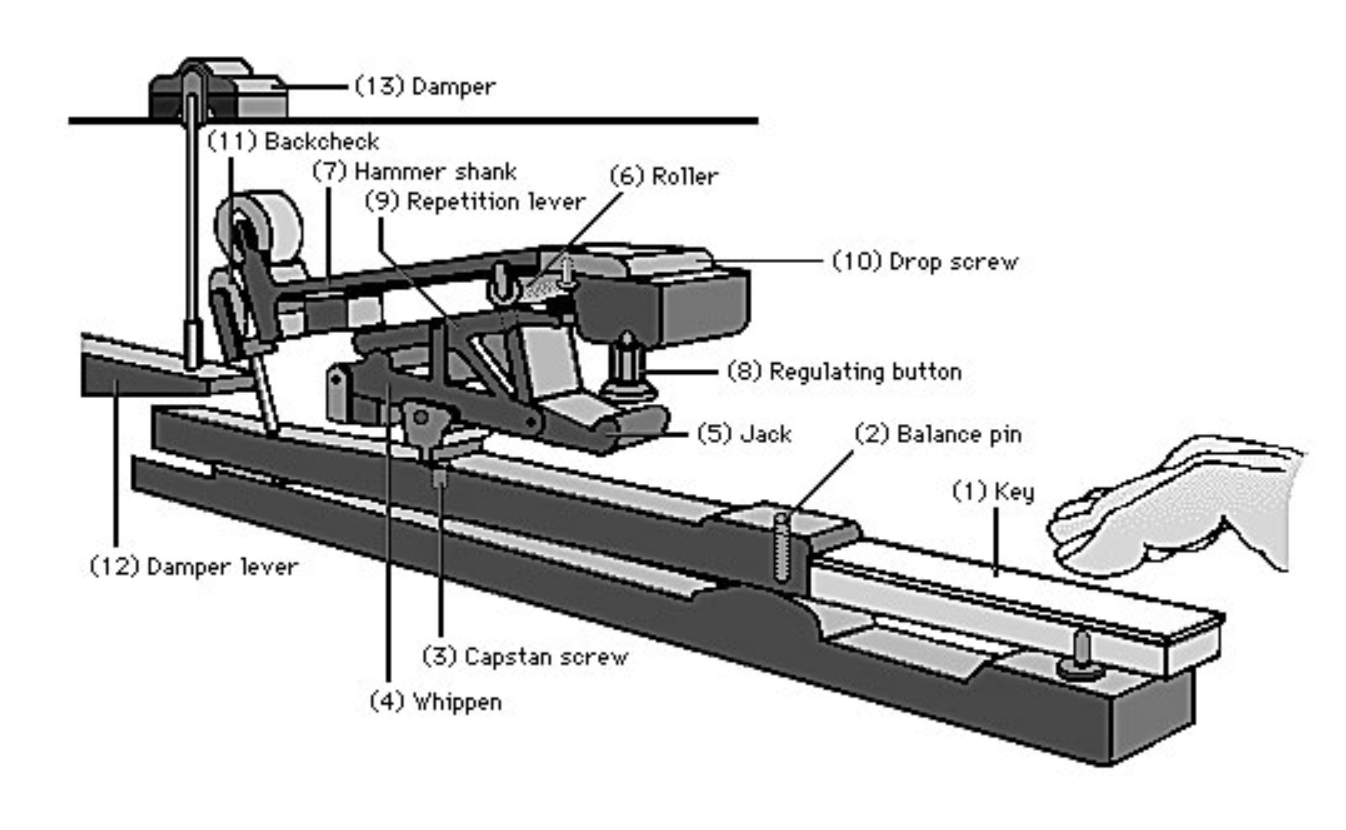
\includegraphics[width=\linewidth]{image/KeyMechanism.png}
  \caption{Grand Piano Actuation Design}
  \label{fig:key_mechanism}
\end{figure}

In a perfect world, the keys of any digital piano (also known as an electric keyboard, keyboard, or synthesizer) would feel, function, and look like an acoustic keyboard. Most players that choose to play a synthesizer, they have most likely played on an acoustic piano. Most keyboard players know that the tactile response of a key in any piano or synthesizer is important because it determines how each note reacts to the player’s touch, this contributes to feel and is often compared to the acoustic piano as the standard. For an example of key feel, lighter keys will respond more quickly to the musician's touch, but will reduce the ease of creating a dynamic range in stroke velocity compared to their heavier counterparts. Extension Spring keys will provide a more uniform but less natural tension throughout the keystroke, compared to acoustic weighted keys with hammers that are balanced on a “balance pin” and separates the user from its striking mechanism. This hammer mechanism is shown in \textit{Figure \ref{fig:key_mechanism}}. The normal force varies more greatly during the press of this key due to this acoustic striking mechanism, but feels natural and provides a wider dynamic range as well.

In addition, each performer and their use of the instrument plays a role in determining the desired preference of key feel. EDM or heavily synthesized music designers will care less about the acoustic key feel because most of the work when writing this type of music, other than determining the melodic structure, will come in post-production and adjusting the key inputs from the computer. On another end of the player spectrum, classically trained musicians will dramatically care about the acoustic key feel because most of the work is dedicated to how they express the music through their performance.

\begin{figure}[h!]
  \centering
  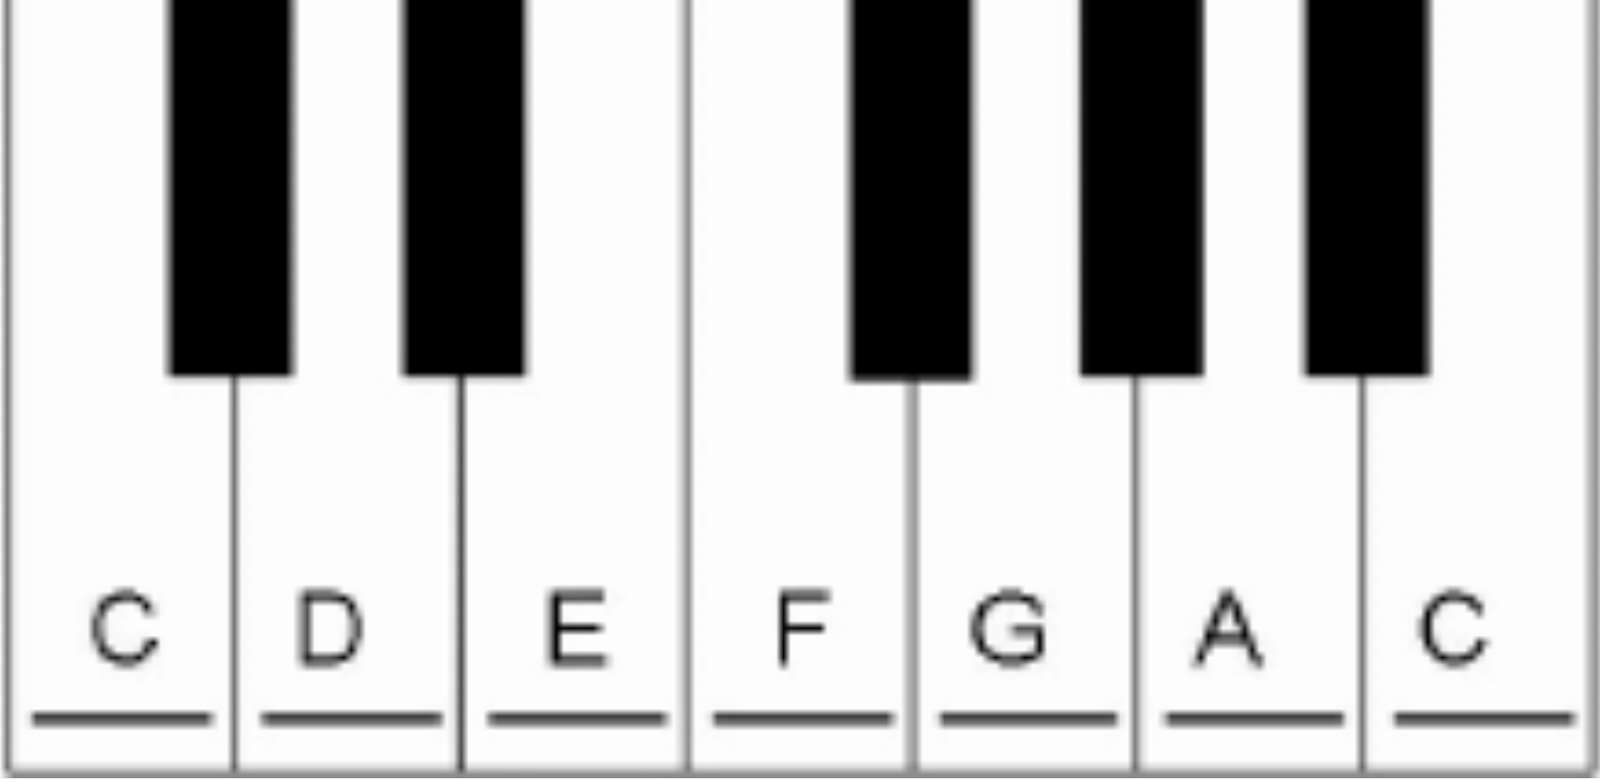
\includegraphics[width=0.5\linewidth]{image/Octave.png}
  \caption{One Octave of Keys}
  \label{fig:octave}
\end{figure}

On top of key feel, the amount of keys available to the player has its own important role to the user and their desired end goal. To gather a better understanding, a single octave on a piano consists of twelve keys: seven white (natural) keys, and five black (non-natural) keys as shown in \textit{Figure \ref{fig:octave}}. A writer who is focused on beat making and synthesized music can craft most of their pieces with a single octave and the use of transposing that octave. A writer who is classically trained will most likely be adjusted to a standard 7 octave keyboard without the option of transposition. With consideration of what will be possible for us, we used this information and decided our device should be modeled similarly to a professionally designed MIDI controller that is smaller than five octaves to keep the portability, but larger than one octave to provide a useful range to more players. We also know that most keyboards do not terminate their key set with a non-natural key, this is discussed further throughout the following sections of this document.

\subsubsection{Key Size}
We created our key design by referencing two distinct electric keyboards: the \textit{Roland DP-90} and \textit{Arturia’s Keylab MkII - 61 key}. We took our initial key measurements from these devices because our group has direct access to these keyboards and there are no official standardized key sizes. Our objective is to empower any creative or independent writer, so these devices were happily chosen in particular for their range of use cases. The \textit{Roland DP-90} is designed such that it “performs and responds like a grand piano”, while the \textit{Keylab MkII} is designed as a “definitive MIDI controller keyboard ... a luxurious, expressive tool for your studio” . By taking measurements from two vastly different devices and noticing the minimal variation between their two key sizes, we were able to be confident that our key size choice would suffice. Although \textit{Figure \ref{fig:octave}} does not express the nuances in key design, there are six different key shapes that we have labeled: black, b, t, d, tb, and td, from the letter shapes they are most similar to. tb and tb are a hybrid of the t and b or t and d shape keys. The measurements taken from those devices are shown in \textit{Table \ref{Tab:key_dimensions}}.

\begin{table}[]
  \centering
  \resizebox{\textwidth}{!}{%
    \begin{tabular}{|l|l|l|l|}
      \hline
      Keyboard                & Roland DP-90 & Keylab MkII & Our Choice \\ \hline
      Black Key               &              &             &            \\ \hline
      Base Width (mm)         & 12           & 12          & 12         \\ \hline
      Base Length (mm)        & 95           & 80          & 80         \\ \hline
      Top Width (mm)          & 9            & 9           & 9          \\ \hline
      Top Height (mm)         & 88           & 72          & 72         \\ \hline
      Standard White          &              &             &            \\ \hline
      Base Width (mm)         & 22           & 22          & 22         \\ \hline
      Base Length (mm)        & 150          & 130         & 130        \\ \hline
      b cut-in (mm)           & 9            & 8           & 8          \\ \hline
      t cut-in (mm)           & 4.5 / 4.5    & 4 / 4       & 4 / 4      \\ \hline
      d cut-in (mm)           & 9            & 8           & 8          \\ \hline
      tb cut-in (mm)          & 3 / 6        & 3 / 6       & 3 / 6      \\ \hline
      td cut-in (mm)          & 6 / 3        & 6 / 3       & 6 / 3      \\ \hline
      Key Separation (mm)     & 1.5          & 2           & 2          \\ \hline
      Trigger Angle (Degrees) & 6.972        & 8.296       & 5          \\ \hline
    \end{tabular}}
  \caption{Keyboard measurements.}
  \label{tab:key_dimensions}
\end{table}

\subsubsection{Number of Keys}

We chose to create a twenty-nine-key keyboard. We landed on this choice as a result of the following factors: first, when this device is in use we do not wish to limit our users to one octave. Our autocomplete AI is modeled from a variety of music, and we understand that the input and output melodies will likely span over a wider range than one octave. We also recognize that this device is more useful in the post-production setting compared to a performance setting and therefore does not need the full seven octave range. Second, to keep the cost low and the form factor small, we wanted to keep the keys below three octaves. We are choosing to build this keyboard as a portable, stand-alone piece of equipment and we believe our device should not cause struggle to carry around. With the measurements we took, each octave will accompany about 262 mm (10.315 inches) of space in keys alone. This means a twenty-nine key keyboard is estimated to need 633 mm ($ \approx $ 2.08 ft) of lateral space in keys alone. We knew when multiplexing our signals that twenty-nine keys provide a set of two and a half octaves and will utilize the entirety of each multiplexor without extending the keyboard to sixty keys, which is around five octaves. To compare, sixty-four keys would extend to 1313 mm ($ \approx $ 4.3 ft) and in our humble opinion, would no longer allow this device to be comfortably portable.

\subsubsection{Key Functionality}

In our application we are looking to distinguish which note is being pressed, the velocity that note was triggered, and which channel the device is communicating through. With the digital functionality of the key in mind, the physical key design only has to worry about how to communicate the velocity of the note to the Arduino, which will later be sent to the Pi. To be able to do this, we are using a two button trigger system for each key. As observed in \textit{Figure \ref{fig:key_mechanism}}, there are two rods extending from the bottom of the key of different lengths. In the full keyboard model, these rods are lined up with two silicone covered buttons with printed button caps. The button furthest from the player is triggered at the start of the keystroke and the other is triggered near the conclusion of the keystroke. The difference in trigger time between the two buttons will determine the note velocity.

Following basic functionality, our next concern is key feel. With the time allotted for this project, the feasible options when crafting at our level of expertise, and our desire for ease of portability, it is for obvious reasons after observing \textit{Figure \ref{fig:key_mechanism}} that we will not attempt to replicate the full counter-weighted key design. The size of the full hammer mechanism is too large and the design expands far beyond our ability. To keep costs low and durability high, we are also avoiding any semi-weighted keys or the usual expensive key material such as ivory or wood. By utilizing 3D printed plastics, we are able to create custom, robust designs at a cheaper cost than the alternatives.

To provide the actuation action for the key itself, we will be using tension springs to hold the key in place as it sits on a lever rail. A platform behind the rail will be installed to prevent any negative actuation and a chassis will be designed to hold the key rail.

\subsection{Prototyping}

\subsubsection{Keyboard}

Before deciding the selection of tension springs, actuator lengths, and the peripheral components to complete the key functionality, we knew that a few initial designs and test prints should first be created and printed to ensure our future endeavors would work as planned. With 3D printing, especially while utilizing an ‘at home’ 3D printer, there are a few parameters we need to keep in mind.

\begin{figure}[h!]
  \centering
  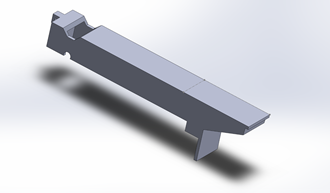
\includegraphics[width=0.7\linewidth]{image/WhiteModel1.png}
  \caption{Natural Key Base Model}
  \label{fig:white_model1}
\end{figure}

An associate of the team built the 3D printer we will be putting to use. Due to the years of development, custom embedded code, and a variety of parts from different manufacturers, the best resource to learn about the printer would be our associate himself: Anton Strickland. Anton’s printer was initially purchased as a Creality Ender 5. The first major change to the hardware was the replacement of the control board from an eight bit control board with fifteen kilobytes of memory to a thirty-two bit control board with 512 kilobytes of memory. The increase in processing power along with the increase in memory allows for some advanced features such as enhanced acceleration control, jerk reductions, and square wave output.

The enhanced acceleration control as well as the jerk reduction are important parameters for the speed of the print. We will be sharing this printer with other groups and since we plan to print possibly more than thirty-one keys, the key rail configurations, and the electronics housing, it is important to make sure the prints will be executed accurately and produced in time to be added to the prototype. The enhanced acceleration control allows the device to change velocity with more precision and boost our confidence to ramp up the speed of the print where at all possible. As a result of attempting more speedy prints, the jerk, or change in acceleration, needed to be monitored more greatly as well. With the new control board, reducing the jerk and altering the extrusion rate of the filament with the newly enhanced parameters is finally possible. In addition to these parameters, the new board can signal using square waves as an output. This means the data that we are sending and monitoring is more consistent and reliable. All together, this means faster prints with a smaller rate of failure compared to the previous board.

In addition to the hardware that boosts the software, this device is equipped with 2209 Stepper motor drivers which replaced the original drivers to add smoother and consistent nozzle travel. The nozzle has also been replaced with an upgraded hot end titanium heatbreak nozzle that is designed to prevent heat creep. This is important when printing multiple prints in rapid succession to prevent any overheating or inconsistent filament extrusion. This also means that the printer can print twenty-four hours a day and seven days a week without a high risk of print failure.

The hardware Z-axis lead screw has also been replaced from four-hundred steps per millimeter to 1600 steps per millimeter, increasing the accuracy of layer size and decision variation. This device can print anything smaller than 220x220x400 mm, a line width that can be altered from .2 mm to .8 mm with as small as +/-.15 mm tolerance, and customizable infill percentages.

From this information, it is evident that most prints with any structural integrity will be indefinitely feasible as long as each print is smaller than the allotted max size of 220x220x400 mm.

To begin crafting the keys for this device, I started with a basic model I have labeled textit{WhiteKeyStart.SLDPRT}, shown in \textit{Figure \ref{fig:white_model1}}. The white keys, also known as natural keys named after the not sharp nor flat notes in music, are the longer set of keys which make up most of the space on the keyboard. As you can see from \textit{Figure \ref{fig:white_model1}}, this key does not have the actuating levers to connect to the buttons on the PCB nor does it have any cuts to make room for the black keys, or non-natural keys, which fit in-between most of the white keys. This model was crafted from measurements and observations made from \textit{Table \ref{Tab:key-dimensions}} and is the baseline of each natural key model. Looking at the model in \textit{Figure \ref{fig:white_model1}} closely, one can observe the incomplete sketch line that is about one-third into the key. This sketch marks the location where each key needed to be cut, forty-eight millimeters from the base, to create the five different models of the natural keys and ultimately allowed the crafting of the following models to be much easier.

The major parameters of this model are as follows. Each natural key has a base width of twenty-two millimeters and a playable length of 123.71 mm which is a little shorter than the measured length of the \textit{Keylab MkII}, but fits the idea of the project due to our desire to create a portable device. Viewing \textit{Figure \ref{fig:white_model2}}, we can see that there is a two millimeter lip on the end of the key, shown in the top right of the figure, to create the correct key feel and provide the user with better feedback to distinguish the tip of the key. Below that lip is a five millimeter drop at a 95 degree angle, followed by a 20 degree 28.73 mm drop to provide aesthetic distance from the lip and prevent the key from looking blocky from the front perspective.

Next we can see the functional aspects of the design. Below the 28.73 mm 20 degree decline is a 22 mm guiding plane that is two millimeters thick. This serves not only as a guiding plane, but also prevents the user from viewing the hidden electronics beneath the key. 15 mm up from the bottom of the guiding plane is a 10 mm long platform that is used to limit the actuation of the key for a realistic ten degree actuation angle which will become more apparent in the full model.

\begin{figure}[h!]
  \centering
  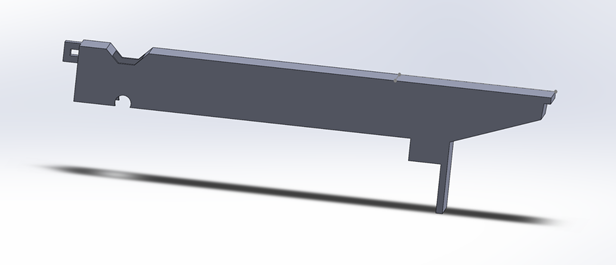
\includegraphics[width=0.8\linewidth]{image/WhiteModel2.png}
  \caption{Natural Key Base Model 2}
  \label{fig:white_model2}
\end{figure}

In the first iteration, the almost complete circle to the far left is five millimeters in diameter. This will be touched on later in this design section of the document. Above that circle is a divot, in the shape of an upside trapezoid, five millimeters at the base with 45 degree inclines to the top of the key. This divot is used to allow the cover of the keyboard to not only help guide the key and keep it in place, but also to once again prevent the user from clearly seeing the electronics hidden inside the full device. Finally, on the far top left of the key is a 3x2x5mm hole designed to hook onto the tension springs that help provide the pull-back of the actuation. Each natural key has the exact same cut-in values as given in \textit{Table \ref{Tab:key_dimensions}}.

Next in the first iteration of key designs is the non-natural key, or black key, named after the sharp and flat notes these keys trigger. From a design standpoint, it is helpful that all the non-natural keys share the same structure. To begin, the guiding plane and size of the connecting platform have the same measurements of the natural keys, a fifteen millimeter plane and a ten millimeter platform. The divot, the hole beneath the divot, and the extruded cut where the spring attaches all have the same measurements as the natural keys as well. The original design has a playable length of 120.71 mm. Due to the shorter playing length and same guiding plane length, the actuation of the keys has been approximated to be around 15 degrees, compared to the 10 degree actuation of the natural keys. This key does not need any tip as a tip could obstruct any transition the player may have switching from the non-natural keys to the natural keys, instead the tip of the non-natural key has a 15 degree chamfer on all sides to allow the fingers to slide from the elevated top of the non-natural key to the lower natural keys. As a result, the top of the key is thinner than the base, as is expected from the measurements taken in \autoref{tab:key_dimensions}. To gather a better understanding, the base of the key is the section which aligns with the elevation of the natural keys, while the tip elevates ten millimeters above the key. Between the base and the tip is what makes up the key itself.

\begin{figure}[h!]
  \centering
  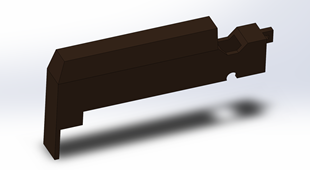
\includegraphics[width=0.7\linewidth]{image/BlackModel.png}
  \caption{Non-Natural Key Base Model}
  \label{fig:black_model}
\end{figure}

The first iteration of the key rail and base was intended to be a completely 3D printed component shown in \textit{Figure \ref{fig:base_model1}}. This rail and base, filed as KeyRail2.SLDPRT, features a five millimeter thick base for structural integrity with an overall length of 94.5 mm to allow the guiding plane of the natural keys to sit in front of the base itself. The six millimeter extruded cuts, which occur 76.5 mm from the back of the base, are to allow the guiding planes from the black keys to slot within the holes freely and without obstruction. There is a 10 degree incline at the front of the base and a 10 degree incline near the non-natural key guiding holes, which is addressed later, to give the keys a flat plane to stop the actuation when the keys are fully pressed to play. The rail that the keys attach to, which is raised 27.83 mm from the back of the base to the center of the rail, is 4.85 mm in diameter and has two millimeter plastic spacers at appropriate distances to slot each key into position while allowing enough space to easily actuate. In this design, I allowed one millimeter of tolerance for each key. This rail is supported by 2.5x2mm thick vertical poles with a 2.5x3 mm horizontal piece of support plastic. When assembled, the full first prototype can be seen in \textit{Figure \ref{fig:assembled_model}}.

\begin{figure}[h!]
  \centering
  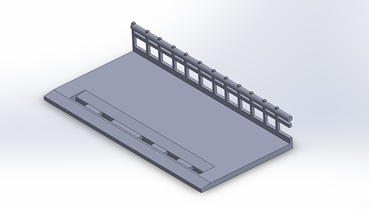
\includegraphics[width=0.8\linewidth]{image/BaseModel1.png}
  \caption{First Iteration Keyrail}
  \label{fig:base_model1}
\end{figure}

To allow an appropriate prototype test, I first chose to simulate the assembly with collision detection enabled. Luckily, while all keys were in their starting position, no collisions were detected. Sadly, when some keys were actuated, the simulation responded with a collision report. It was difficult, at first, to determine where the collisions were occurring. In some settings, it was evident that certain collisions only occurred when the keys were placed in positions that would not be possible in the final assembly and actual implementation of the device. In other cases, the collisions could not be easily seen in the model. Due to this, I decided to run a test print of some of the pieces present. I figured I would not need the entire model to determine where the problems were occurring as the difference in model pieces were not drastic.

\begin{figure}[h!]
  \centering
  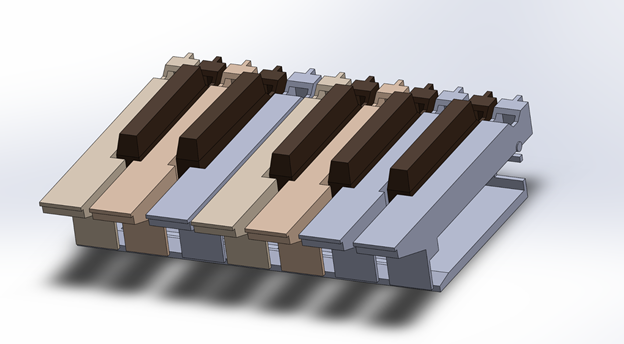
\includegraphics[width=0.9\linewidth]{image/AssembledModel.png}
  \caption{First Iteration: One Octave Design}
  \label{fig:assembled_model}
\end{figure}

\textbf{Iteration One}

This first print was a test to determine the functionality of the keyboard in its preliminary stage. As the reader can tell by the title listed at the beginning of the document, there are no mechanical engineers on this team and therefore there are no members with a solid grasp on tolerances for different applications. We figured the best way to determine the tolerance we are looking for is to test a couple different sizes. In the test print, the rail itself was designed to be 4.85 mm in diameter, so obviously we needed to allow the circular cut which rests on the rail to be larger than 4.85 mm in diameter. For this print, we used the rail, the b-model, the t-model, and two non-natural keys. The b-model had a circular cut of 5.35 mm in diameter, the t-model had a circular cut of 5.15 mm in diameter, and the black keys had a circular cut of 5 mm in diameter shown in \textit{Table \ref{Tab:connections}}.

\begin{table}[]
  \centering
  \begin{tabular}{|l|l|}
    \hline
    Model           & Connection Diameter (mm) \\ \hline
    Rail            & 4.85                     \\ \hline
    b-model         & 5.35                     \\ \hline
    t-model         & 5.15                     \\ \hline
    Non-natural key & 5                        \\ \hline
  \end{tabular}
  \caption{Hinge Hole Test Measurements}
  \label{Tab:connections}
\end{table}

The results of the model are shown in \textit{Figure \ref{fig:print1}} below.

\begin{figure}[h!]
  \centering
  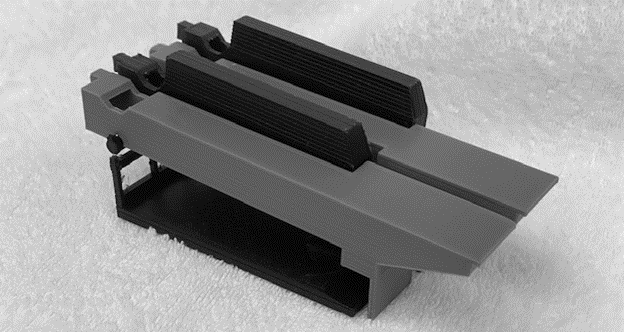
\includegraphics[width=0.8\linewidth]{image/Print1.png}
  \caption{First Iteration: Test Print}
  \label{fig:print1}
\end{figure}

At first glance, the model seemed really well produced. The results of the different tolerances for the connecting circular cut to rail are as follows. With a 0.15 mm tolerance, as exemplified from the non-natural keys, the keys snapped into place and connected with the keyrail. At a 0.3 mm tolerance, the t-key was able to slide, but with resistance. At a 0.45 mm tolerance, the b-key was able to slide with ease. Luckily, the 0.45 mm tolerance did not make the b-key feel shaky or disconnected from the rail which was an issue we hoped to avoid and learn about through this test. From this test, we knew that moving forward with a 0.45 mm tolerance was our best bet. The major issue with this test is that the rail itself is not perfectly round because it is constructed of linear layers and, although it provides a good idea for the final model, is not the best example of how rotational tolerances should be designed. This is addressed in Iteration Three of the prototype.

\begin{figure}[h!]
  \centering
  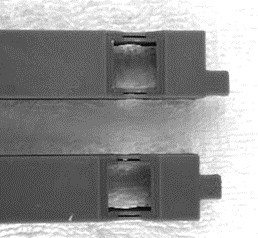
\includegraphics[width=0.6\linewidth]{image/Print2.png}
  \caption{First Iteration: Offset Hook Connections}
  \label{fig:print2}
\end{figure}

After toying with the model for some time, a few issues were brought to light. The most obvious being the uneven slots designed to grip the tension springs, shown in \textit{Figure \ref{fig:print2}}. Since we did not change the base location of the holes to hook the springs, the way the cuts were made created uneven spacing of the aft tip of the key. Not only that, with the holes using 2 mm of wall space and being 5 mm deep, it was evident after the print that those holes needed to be less deep to actually allow the spring to hook. Since the keys are light and the tension of the spring does not need to be exceptionally tight or forceful, it will be more than possible to reduce this thickness without any major issues in functionality.

\begin{figure}[h!]
  \centering
  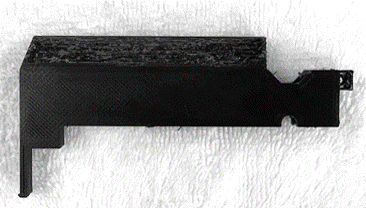
\includegraphics[width=0.8\linewidth]{image/Print3.png}
  \caption{First Iteration: Non-natural Key Test Print}
  \label{fig:print3}
\end{figure}

The next minor fault was with the quality of the print. Due to the chamfered edges of the non-natural keys and the way the model was designed, the key needed support material between the base and the tip of the key. This support material, when removed, caused a rough edge to the key itself, shown in \textit{Figure \ref{fig:print3}}.  To fix this, our team debated a few different ideas. First, we thought about restructuring the key itself and removing the chamfer such that the key could print in a different orientation. This would be additionally helpful because it would allow the key to be printed from the top of the key down, meaning the top plane would be placed on the printing bed leading to a smoother key texture where the user plays. The biggest downside to this idea is that the key would lose its gradual shape from the top of the key and make the key itself look and feel more blocky to the player.

An alternate idea, rather than changing the model, is to simply add a thin layer of epoxy resin to the surface of the key to create that smooth key feel the player will desire. This eliminates the option of a blocky key, but also adds additional work on our end and may cause an uneven surface finish. Another alternative idea is to manufacture these non-natural keys at a professional 3D printing company. This idea has already been debated by the team before the model was even completed, but comes with its own problems of shipping time and extra cost. We ultimately decided an at-home printer would be better. Although the print quality would be significantly less than that of a professional print, it would be easier to make quick adjustments and save money.

Continuing with the non-natural key, another issue reared its ugly head: actuation interference. Since the non-natural keys were designed to be only 3 mm shorter than the natural keys, the natural keys were unable to actuate fully without coming in contact with the guiding plane of the non-natural keys and stopping the actuation of the natural keys. The length of one or the other needed to change and this is discussed in Iteration Three of the prototype.

Another issue we discussed is the fact that there were no parameters in place to prevent the key from actuating backwards. Considering the tension spring will be pulling the key in place, we needed to take into account the possibility that the resting position of the spring will most likely not be the exact distance from the two hooks in the final design. And that we may not even want the resting position of the spring to be of equal length of the two hooks the spring will attach to. This is further touched on in Iteration Three of the prototype.

\begin{figure}[h!]
  \centering
  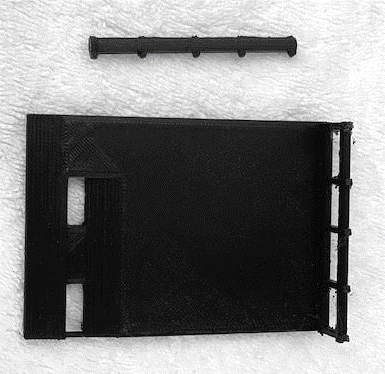
\includegraphics[width=0.8\linewidth]{image/Print4.png}
  \caption{First Iteration: Keyrail Test Print}
  \label{fig:print4}
\end{figure}

The final issue, as shown in \textit{Figure \ref{fig:print4}}, is the poor structural integrity of this completely 3D printed part. Within two hours of the print being completed, the rail detached from the support material rendering the entire print useless. Luckily we were able to receive the results from the test that we needed before the entire print broke down. While discussing the integrity and viewing \textit{Figure \ref{fig:print4}}, it is also evident that creating overhangs that this model demands results in a lot of stringing and print mutations that were not intended.

Thus, it was back to the drawing board, or as SolidWorks users describe, the sketching board, and back to redesigning

One major benefit of this print is noting that an estimated time of printing all thirty-one keys is about two days or 49 hours. Anton, my reference for the printer, states that this can be sped up to about 42 hours for all thirty-one keys if necessary. Due to the alterations made to the printer, this can be a 42 hour print straight through with only adding extra time to remove the print from the bed. This indicates that there will be zero issues regarding timing when it comes to our prints considering we have approximately three months to print and assemble this device.

\textbf{Iteration Two}

As the reader may notice, there are many references from the first iteration to the third iteration. This is because iteration two did not have many major changes, was quickly discussed, and transformed into Iteration Three which is as follows.

\textbf{Iteration Three}

From the results of Iteration One and Iteration Two we decided to alter the length of the non-natural keys to prevent actuation interference between the non-natural and the natural keys. In this design, the non-natural key is 72 mm in base length and 69 mm in tip length. Although this design decreases the length of the non-natural key by about 10\%, we figured this difference would not be an issue as there are no standardized key lengths and this is a collegiate level project. Obviously the base and key-rail design needed to account for this change, but this is not the only change which helped develop this model into the third iteration.

\textit{Figure \ref{fig:base_model3}} shows the file KeyRail3b.SLDPRT. It is obvious when compared to the first iteration that many changes occurred. The comparison of the two versions can be seen in \textit{Figure \ref{fig:base_model2}}.

\begin{figure}[h!]
  \centering
  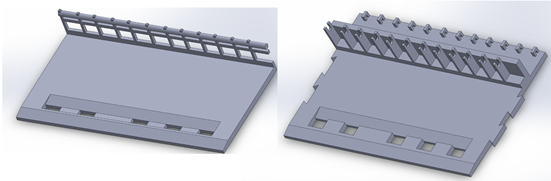
\includegraphics[width=0.8\linewidth]{image/BaseModel2.png}
  \caption{First and Third Keyrail Interation Comparison}
  \label{fig:base_model2}
\end{figure}

The first major change in iteration three compared to that of iteration one is the absence of a key rail. After witnessing the performance of the 3D printed rail and noticing the deformities and the overhangs, we decided to completely eliminate the idea of a 3D printed rail. Instead of a printed rail we are choosing to purchase a stainless steel rod which is discussed in the Component Selection section of this document. By eliminating the rod from being printed we are able to not only utilize a smoother rod to create smoother actuation, but also allow the model to be printed from the base up with only one overhanging section: the spring hook slots. From the model of the natural keys and its test print, however, we know we do not need to worry about these overhangs as they are similar overhangs presented in that model. This is shown in \textit{Figure \ref{fig:print5}}.

\begin{figure}[h!]
  \centering
  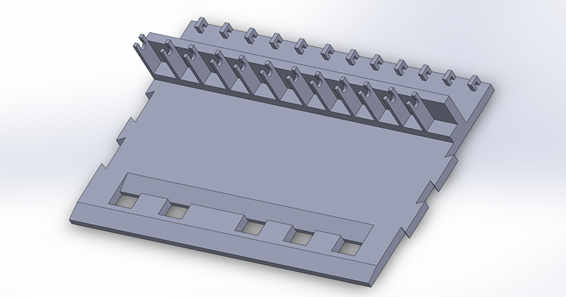
\includegraphics[width=0.9\linewidth]{image/BaseModel3.png}
  \caption{Third Iteration: Full Keyrail Model}
  \label{fig:base_model3}
\end{figure}

Furthermore, discussing the width of the holes for the springs to attach, we have reduced the width from five millimeters to 2.5 mm on both the keyrail base and the keys themselves. This thinner design will allow the springs to hook around the plastic, through the holes, and prevent slipping of the springs. From the test in which we observed the different tolerances of the key rail connection to the keys, we have decided to allow a 0.15 mm diameter tolerance for the metal rod to snap into the chassis. This model, seen in \textit{Figure \ref{fig:base_model3}}, also features a 5 mm wide platform raised 21.83 mm from the base behind the rail itself to prevent the key from rotating past the horizontal plane in the opposite direction. We also changed the support which holds the rod from a 2.5x2 mm pole to a 2x8 mm pole to increase structural integrity. Although, when viewing the keyboard from the players perspective, there is less support in the x axis for these poles, there is significantly more support in the z direction which is where more of the force of the player will be applied. In addition, because we are using a stainless steel rod in the x direction, our device should have more than enough support to operate under normal playing conditions easily.

\begin{figure}[h!]
  \centering
  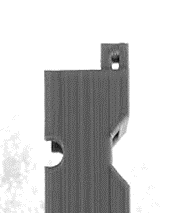
\includegraphics[width=0.25\linewidth]{image/Print5.png}
  \caption{Third Iteration: Key, Hook Connection}
  \label{fig:print5}
\end{figure}

Continuing to discuss \textit{Figure \ref{fig:base_model3}}, the non-natural key incline next to the guiding holes has been altered to 15 degree to better account for the angle of actuation those keys will encounter. We also increased the hole width from 6 mm to 10 mm to provide ample room for the guiding plane on the black to actuate through. Increasing this hole size was also only possible by shortening the key size of the non-natural key and allowing 2.75 mm of 5 mm thick support between the guiding holes for the non-natural keys and the start of the key rail’s base incline for the natural keys.

The final major change shown in \textit{Figure \ref{fig:base_model3}} are the odd protrusions and extruded cuts on the far left and right of the base. After reviewing the printing size limitation of 220x220x300 mm, we knew we could not print the entire keyboard base at once as one octave alone is 192 mm in width and we aim to have a 2.5 octave keyboard. To combat this, we decided to create a design such that the different base pieces could attach like a puzzle. After these pieces are attached, we plan to glue the model together using a ‘3D print-safe’ adhesive and attach a thin vinyl layer to the bottom of the base to create a more professional look.

\begin{figure}[h!]
  \centering
  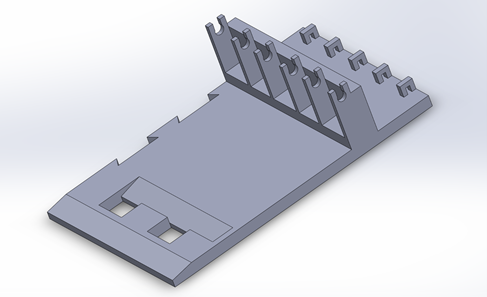
\includegraphics[width=0.8\linewidth]{image/BaseModel4.png}
  \caption{Third Iteration: Half Keyrail Model}
  \label{fig:base_model4}
\end{figure}

Since we are creating a keyboard that is two and a half octaves wide, we also need to create a model for the half octave keyrail shown in \textit{Figure \ref{fig:base_model4}}. This model shares the same measurements as the other keyrail and base model, but terminates at the fifth key’s support beam.
The other change made after observing the print was manually centering the hook hole for each one of the key models. This is shown in \textit{Figure \ref{fig:key_models}}.

\begin{figure}[h!]
  \centering
  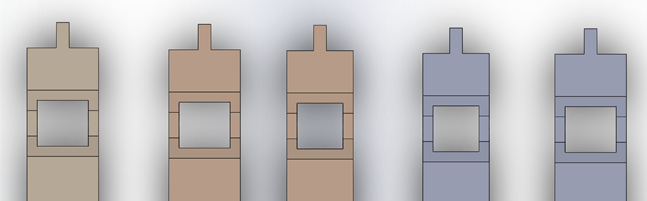
\includegraphics[width=0.8\linewidth]{image/KeyModels.png}
  \caption{Third Iteration: Corrected Hook Connections}
  \label{fig:key_models}
\end{figure}

After testing and reiterating the initial print models, we were finally able to move on to the body of the keyboard itself. Much like the previous prints, we now realized the importance of being able to print from one face up with zero overhangs and this is something we achieved. We also knew our limitation from the printer itself and therefore, the body model is as follows. We needed an elevated base to allow the keys to actuate, a group of printed parts that follow our restrictions as well as attach together, and an area to house the electronics and display.

\begin{figure}[h!]
  \centering
  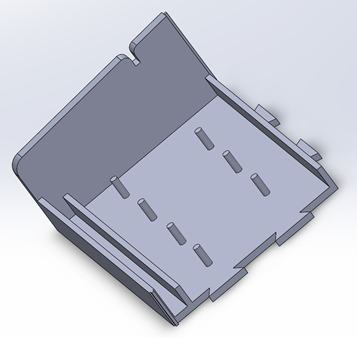
\includegraphics[width=0.8\linewidth]{image/BodyModel1.png}
  \caption{Body Model: 2x1}
  \label{fig:body_model1}
\end{figure}

For the front left base body print we created the model shown in \textit{Figure \ref{fig:body_model1}}. From the player’s perspective, at the very front is a 31 mm tall wall, followed by an 11 mm gap, and then a 16 mm tall wall. This is to help guide the natural key’s actuation and prevent the player from seeing the electronics within the device. It is also a standard set up that most portable electric keyboards have. Within the center are seven poles, each 16 mm tall, and a 16 mm tall wall in the back. Each 16 mm high structure was designed to hold the keyrail above the base, shown in \textit{Figure \ref{fig:body_model2}}, which allows each key the space it needs to actuate. The front and side walls are also equipped with a 1 mm protrusion along the vertical axis of the inner wall, and protrusions similar to that of puzzle pieces to all each section to easily be connected and glued together.

\begin{figure}[h!]
  \centering
  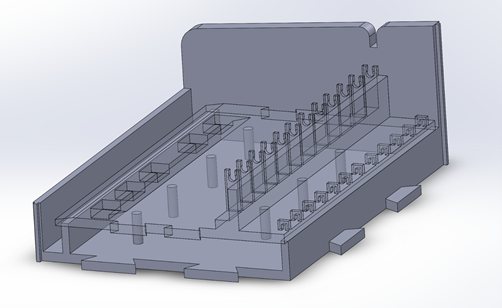
\includegraphics[width=0.8\linewidth]{image/BodyModel2.png}
  \caption{Full Keyboard Body Model with Keyrail Placed Correctly}
  \label{fig:body_model2}
\end{figure}

As can be seen in \textit{Figure \ref{fig:body_model2}}, the key rail, base, and body fit together perfectly, allowing space in the front for the guiding plane of the natural keys.

To the left of the base we see a divot that is 4 mm wide at a variable depth. This divot is to allow the cover to sit comfortably on the full assembly without sliding off. The base of each model is 5 mm from the ground up. The front and inner wall are 4 mm, while the outside walls are all 8 mm thick to provide a robust shell for the device. Also, from \textit{Figure \ref{fig:body_model2}}, we can see that the puzzle-piece-like protrusions do not align from the base to the body. This was intentional to produce a more rigid structure when the device is fully assembled.

\textbf{Assembly}

The full keyboard is about 483 mm wide, 322 mm deep, and 93.89 mm tall. From our printer restrictions of 220x220x300 it is obvious we cannot print this as one full device. To counter the limitations, we divided the keyboard into six different sections in the style of a 2x3 matrix. For our design, the first row is dedicated to the electronics housing and the second row is dedicated to the keys. The body pieces which make up this arrangement are shown below. In \textit{Figure \ref{fig:body_parts}(a)}, we have the 1x1 body piece, in \textit{Figure \ref{fig:body_parts}(b)}, we have the 1x2 body piece, in \textit{Figure \ref{fig:body_parts}(c)}, we have the 2x1 body piece, in \textit{Figure \ref{fig:body_parts}(d)}, in \textit{Figure \ref{fig:body_parts}(e)}, we have the 1x3 body piece, we have the 2x2 body piece, and in \textit{Figure \ref{fig:body_parts}(f)}, we have the 2x3 body piece.

\begin{figure}[h!]
  \centering
  \begin{subfigure}[b]{0.45\textwidth}
    \centering
    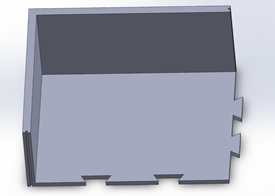
\includegraphics[width=\textwidth]{image/BodyModel3.png}
  \end{subfigure}
  \begin{subfigure}[b]{0.45\textwidth}
    \centering
    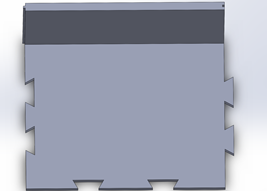
\includegraphics[width=\textwidth]{image/BodyModel4.png}
  \end{subfigure}
  \begin{subfigure}[b]{0.45\textwidth}
    \centering
    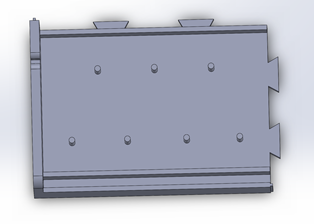
\includegraphics[width=\textwidth]{image/BodyModel5.png}
  \end{subfigure}
  \begin{subfigure}[b]{0.45\textwidth}
    \centering
    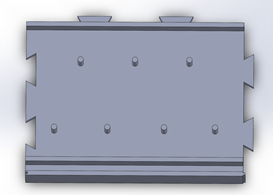
\includegraphics[width=\textwidth]{image/BodyModel6.png}
  \end{subfigure}
  \begin{subfigure}[b]{0.45\textwidth}
    \centering
    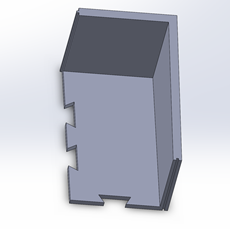
\includegraphics[width=\textwidth]{image/BodyModel7.png}
  \end{subfigure}
  \begin{subfigure}[b]{0.45\textwidth}
    \centering
    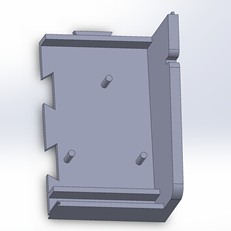
\includegraphics[width=\textwidth]{image/BodyModel8.png}
  \end{subfigure}
  \caption{Individual Body Model Pieces [1x1 - 1x3] and [2x2 - 2x3]}
  \label{fig:body_parts}
\end{figure}

As can be seen from these figures, each piece has been specially crafted to fit into each other like a puzzle. We can see the full arrangement of the assembled body in \textit{Figure \ref{fig:assembled_body}}.

\begin{figure}[h!]
  \centering
  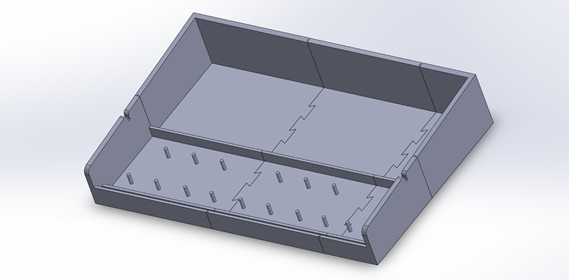
\includegraphics[width=0.9\linewidth]{image/AssembledBody.png}
  \caption{Full Keyboard Body Model}
  \label{fig:assembled_body}
\end{figure}

This body allows for the keys to be elevated, keeps the bottom of the device level, maximizes the space for the electrical components, and protects the components inside. The front of the device starts at a max height of 63.42 mm and creates a 10 degree incline until the back of the device maxing out at 93.89 mm in height.

The cover or front panel of this device is 483x196.5 mm. There is absolutely no way to print this with our at home printer. Our front panel is shown in \textit{Figure \ref{fig:display_model}} and features five separate extruded cuts.

\begin{figure}[h!]
  \centering
  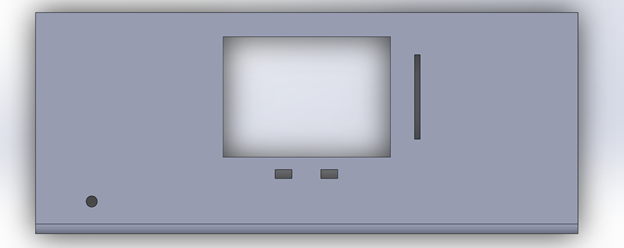
\includegraphics[width=0.9\linewidth]{image/DisplayModel.png}
  \caption{Front UI Panel: Keyboard}
  \label{fig:display_model}
\end{figure}

In the center of the front panel is a 149 mm by 107 mm hole to house the seven-inch capacitive touchscreen display. To the right of the display slot is a 5 x 75 mm slot designed to house the sliding potentiometer which will be used to control the volume of the device. Below the screen are the two holes where the octave up and octave down buttons will be placed and in the button left of the cover is where the audio jack for the user’s headphones to plug in will be installed.

Since the user interface will be controlled by a touch sensitive screen, we placed the slot equally spaced from the left and right of the cover to be able to equally treat left and right handed individuals. All the buttons and potentiometers surround closely as well for ease of use. The headphone jack was placed in its location because many over-ear headphone companies produce headphones with the wire extending from the left ear in hopes to avoid obstructing the right hand, which is the majority of the population’s dominant hand. Ultimately, everything needed a place and we felt these locations were the best fit.

When all the parts are connected and in place, the intended design of the body can be seen in \textit{Figure \ref{fig:final_model1}}. With the keys in place, the full assembly and design on the keyboard can be seen in \textit{Figure \ref{fig:final_model2}}.

\begin{figure}[h!]
  \centering
  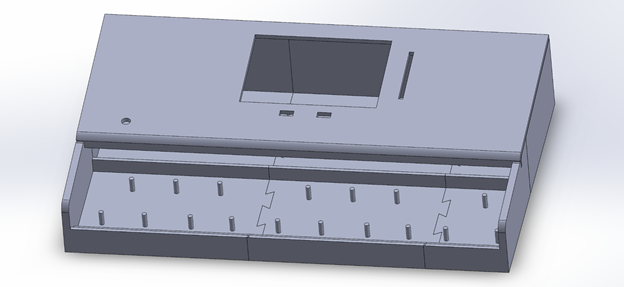
\includegraphics[width=0.8\linewidth]{image/FinalModel1.png}
  \caption{Fully Assembled Keyboard Body}
  \label{fig:final_model1}
\end{figure}

\begin{figure}[h!]
  \centering
  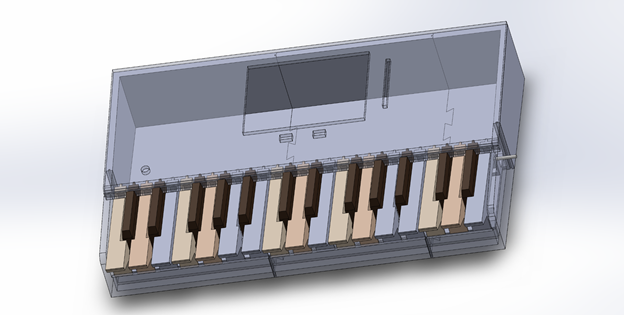
\includegraphics[width=0.8\linewidth]{image/FinalModel2.png}
  \caption{Fully Assembled Keyboard Model}
  \label{fig:final_model2}
\end{figure}
\clearpage

\textbf{The Final Iteration}
Sadly, by the time the final documentation was written, our SolidWorks license expired. The following notes will not have accompanied models, but will discuss the final altercations before assembling the keyboard.

The key design only had slight alterations from the Third Iteration. The most notable of these changes were the actuation rods which pressed the silicon buttons over the duration of the keystroke. These were 5 mm diameter cylindrical rods which extended down such that the back rod would trigger the back button slightly before the front rod would trigger its accompanying button. The hole which connected the key to the metal key-rail was finalized at 4.35 mm to create an inescapable slot which also allowed the key to rotate freely about. To reinforce the keys, we did not use any type of epoxy. We found that using the print bed as the top of the key would create a smooth surface that was enjoyable to touch. To reinforce the rest of the key we strategically filled the points which receive the most tension with hot glue. This adhesive provides durability and flexibility to the load bearing points.

Sadly, for the key functionality, after days of troubleshooting we could not get the keys to reliably make contact with back buttons. Due to the silicon tops of the buttons, they required actuation that comes down with nearly perfect accuracy around five degrees. Since our device actuates by rotation, we could not have the rails make perpendicular contact with buttons to create a consistent closed contact and response. Even after adding the PLA+ button covers to increase the surface area of contact, the only consistent responses were from the front buttons. After reviewing our options, we decided it would be best to remove the velocity function for the sake of most reliable playability.

The final keyrail had the most changes in its design. Due to the size of the PCB and how it was designed, we had to cut most of the keyrail down to its functional parts. What was left was the chassis and the hooks. The chassis was glued to the PCB on a wooden dowel and the hooks were glued to the inside of the body model on a sheet of wood. We ended up using 2.5 in x .25 in x .035 in zinc plated extension springs to create the actuation.

The body itself did not change, but the cover had slight alterations. Below the screen we added two more buttons and three holes on the far left of the cover. The top hole is to slide a wire through which connects the device to the computer, the second hole down is for the button which turns on the device, and the third hole down is for the slot where the device can be charged. Below is the picture of the final device.

\begin{figure}[h!]
  \centering
  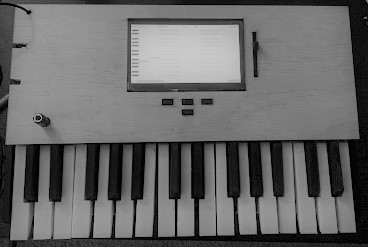
\includegraphics[width=0.8\linewidth]{image/Keyboard_Photo.jpg}
  \caption{Built and Assembled Live Keyboard}
  \label{fig:keyboard_photo}
\end{figure}

\subsubsection{DAW: Static}

Our DAW prototype was constructed without the use of the Electron UI-building environment. This
decision was motivated by the belief that creating the Electron application encompassed two
separate problems: the first was to create a fully functioning script, the second was to port that
script into the Electron application. By building the prototype outside of Electron, we aimed for
faster progress and less bottlenecking of the workflow by dealing with one smaller problem at a
time. Additionally, this decision expedited the debugging process by removing the need to load
the full Electron application every time we wished to monitor the progress of the build. Instead,
we could simply locate the HTML file in out directory and open it in a browser with a single click.

The first step in constructing the DAW was to establish all the static elements, which include
the piano roll (which is displayed inside a horizontally-scrolling container), the guide keys, and
the menu buttons.

\paragraph{The piano roll} is the space in which the user can design their MIDI by adding,
moving, and removing notes. It appears as a rectangular space adorned with horizontal stripes. Each
white stripe corresponds to the vertical position that represents a white key on the keyboard, and
the same goes for the black stripes corresponding to black keys. Progressing upward in the pattern
of stripes is equivalent to progressing left to right on the keyboard. The guide keys follow a
similar format to the piano roll, with black and white stripes that visualize a piano keyboard
rotated 90 degrees counter-clockwise. Unlike the piano roll, however, the guide keys are much
shorter in width and remain as a static element outside (to the left) of the scroll container.
The stripes also display the name of the note to which they correspond. This allows the guide keys
to act as a reference for the user, so they can easily see which note each piano roll stripe
represents without having to count from the bottom. To serve this purpose properly, it is
imperative that the guide keys' stripes line up exactly with those on the piano roll.

This was achieved by building both assets using the same grid display class, given the name
"piano-container." In the CSS script, the piano-container class was styled as a grid display,
which established the appropriate pattern of black and white key items and set a standard gap of
one pixel between each key. The key items were then added as rectangular DIV objects with the
appropriate background color and a standard height of ten pixels. The guide keys were assigned an
additional class called "keys," which gave them a set width. Text was added in the center of each
DIV, labeling it by note. The piano roll was assigned the additional class "roll," which lowered
the opacity of the stripes to allow for better readability. The roll class also gave the piano roll
the absolute position attribute which allowed it to scroll within the scroll container.

At this stage of development, the dimensions of the screen upon which the DAW was to be displayed
were unknown. To proceed with prototyping at a timely pace, we made the width of the piano roll
flexible by reading the size of the window upon opening and setting the piano roll's width
attribute relative to the result. This means that the dimensions may not function properly if the
window is resized after opening, but this is not expected to be a problem because there will be
no way for the user to change the window size on the final keyboard.

\paragraph{The menu buttons} were added below the scroll container, separated into one group which is flush
left, and another which is flush right. The left button group deals with the state of the piano
roll; these buttons allow the user to save the state, reset it to its last save, and utilize undo and
redo functions to return the piano roll to a previous state. There is also a tempo button which
allows the user to select the tempo of playback. The right button group deals with the mode of
interaction. Depending on which of these buttons is selected, the users will be able to switch
between adding, deleting, moving, and stretching the notes on the roll. There are also play and
stop buttons that control playback, and a quantization button that can change the size and
positions the notes will snap to when editing. There is one additional button not included among
the menu buttons. This button exists on the far right of the piano roll, labeled with a plus sign.
It allows users to extend the piano roll so that they may create a longer melody.

\begin{figure}[h!]
  \centering
  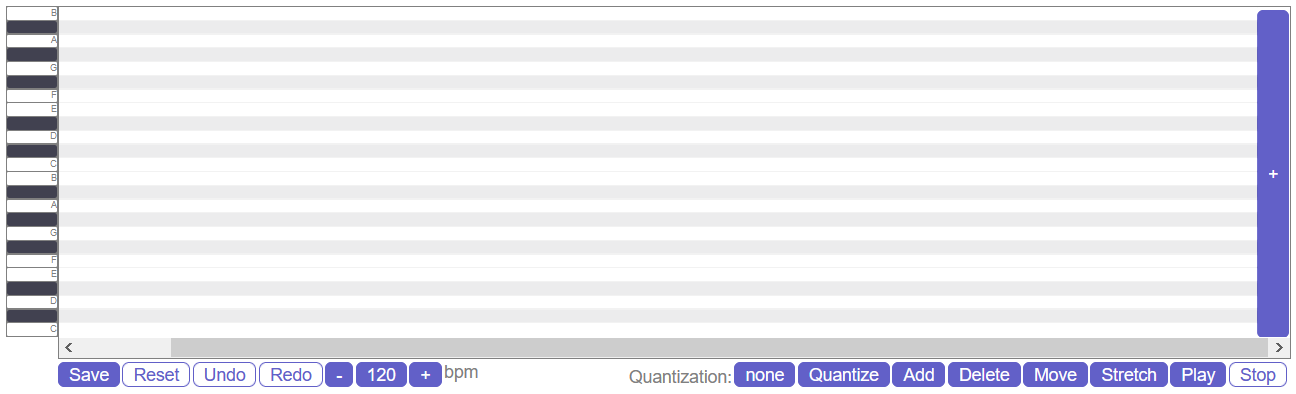
\includegraphics[width=\linewidth]{image/Static.png}
  \caption{A snapshot of the prototype of the DAW, the piano roll is empty.}
  \label{fig:static}
\end{figure}

All UI buttons belong to the CSS class "ui," which gives them a uniform design. This class adds
several cosmetic elements to enhance the user experience by making interactions more visually
pleasing. The buttons have a periwinkle color and rounded corners to make them feel softer and
more polished than the default HTML button. They also expand in size and invert in color when
moused over to indicate they can be clicked. To make this transformation feel fluid, the transition
time has been set to 0.4 seconds, as opposed to the default 0 seconds which would have the buttons
snap immediately from one state to the next. Buttons that are disabled and cannot be clicked are
displayed at the standard size but with inverted colors.

\begin{figure}[h!]
  \centering
  
\includegraphics{image/StdUI.png}
  
\includegraphics{image/HoverUI.png}
  
\includegraphics{image/DisabledUI.png}
  \caption{A sample of the styling of the menu buttons in their standard, hover, and disabled states respectively.}
  \label{fig:ui_variations}
\end{figure}

The quantization and tempo control buttons take on a special structure. Clicking on either of
these buttons opens a drop-down menu from which the user may select a value. The tempo menu
provides options ranging from 30 to 300, but only lists multiples of 20. This is for the
convenience of the user; although they can select any tempo between 30 and 300 by incrementing or
decrementing using the “-“ and “+” buttons on either side of the tempo menu, the drop down allows
the user to skip through by larger units to expedite the process. The quantization button provides
options in the form of note lengths, with the largest being 1/1 and the smallest being 1/64. This
sets the size of the snap-grid on the piano roll relative to the size of a whole note. For example,
if the quantization was set to 1/1 and the user were to move a note, the note would snap to units
of 64 pixels on the horizontal axis because that is the length of a whole note. If the quantization
was set to 1/2, the note would snap to units of 32 pixels on the horizontal axis because that is
half the length of a whole note. Additionally, if the user were to click the “Quantize” button
after selecting a quantization value, all of the notes that are already on the piano roll would
immediately snap to the same units, as demonstrated in \textit{Figure \ref{fig:twinkle_quantized}}.

\begin{figure}[h!]
  \centering
  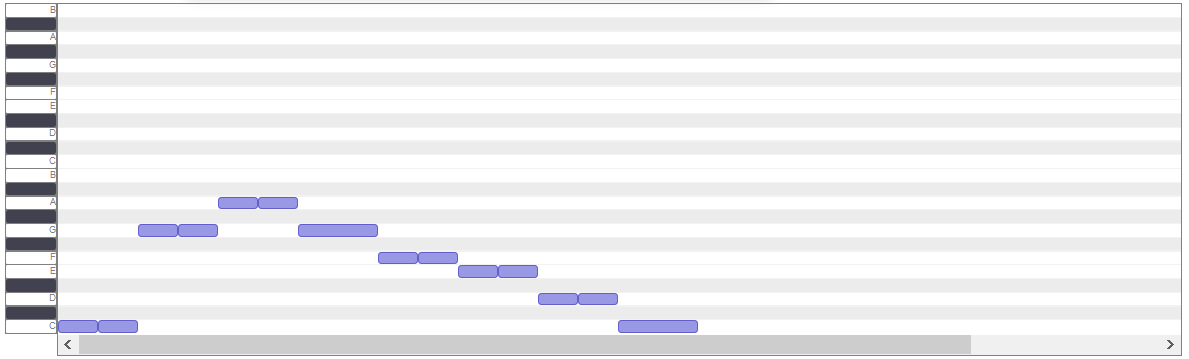
\includegraphics[width=\linewidth]{image/TwinkleOriginal.png}
  \caption{A piano roll displaying the default \textit{Twinkle, Twinkle, Little Star} melody.}
  \label{fig:twinkle_original}
\end{figure}

\begin{figure}[h!]
  \centering
  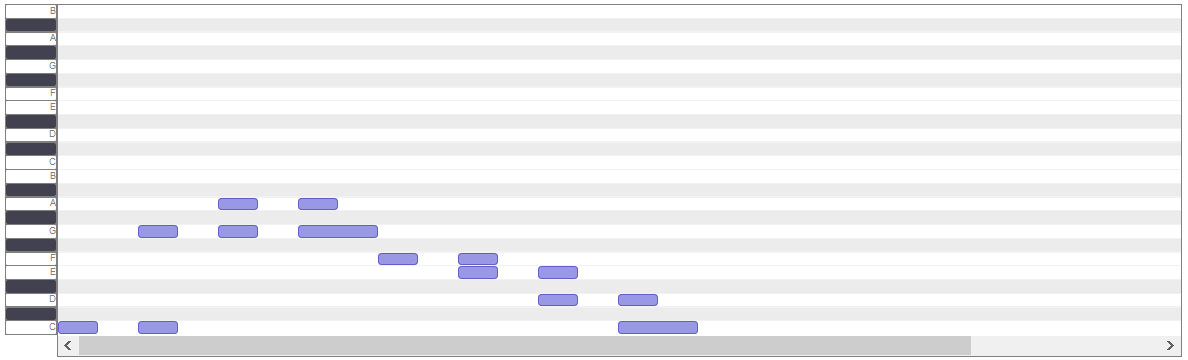
\includegraphics[width=\linewidth]{image/TwinkleQuantized.png}
  \caption{The same melody, now quantized to snap to half-note intervals.}
  \label{fig:twinkle_quantized}
\end{figure}

The drop-down menus were achieved by adding a vertically-scrolling div containing all the menu
options positioned so that the top option layers exactly over the button. This div has an initial
display attribute of “none,” so although all of its styling and position data are active, it is
neither visible nor interactable. Pressing the button sets the menu display attribute to “block,”
which causes the menu to appear over the button and allows the user to interact. Clicking on a menu
item will update the piano roll settings and reset the menu display to “none,” making it disappear
and leaving only the button which will then be displaying the selected menu item.

\begin{figure}[h!]
  \centering
  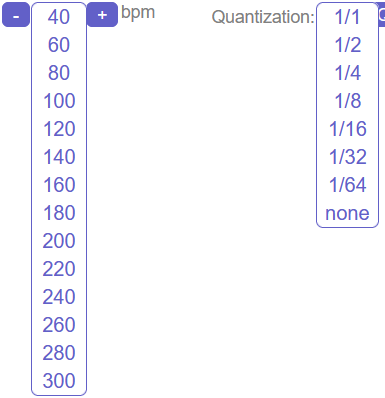
\includegraphics[width=0.4\linewidth]{image/Dropdowns.png}
  \caption{The expanded drop-down elements.}
  \label{fig:dropdowns}
\end{figure}

UI buttons are enabled and disabled on a situational basis to prevent the user from interacting
with the application in an unintended manner. For example, the "Undo" button is disabled if no
edits have been made to the notes or if the user has reverted state using this button more than
the allotted number of times with no edits between. This prevents the user from reverting state
farther back than the original state upon opening. Similarly, the "Redo" button is disabled until
the "Undo" button has been pressed and disables again when any edits are made to the notes. This
prevents the users from redoing an undone state after an edit has been made, thus overwriting any
edits made since the "Undo" button was used. The "Reset" button is disabled only when the program
has just been opened or reset and no edits to the notes have been made since. This is not so much
to prevent the user from pressing it again, but more so to indicate to the user that resetting the
state again would be unnecessary and redundant. The "Play" button is only disabled when
the MIDI playback is active, while the "Stop" button behaves oppositely. Much like the "Reset"
button, this is primarily designed to indicate redundancy in an interaction, but also if the "Play"
button were to be pressed during MIDI playback, a second audio instance of the MIDI would begin
playing over top of the first. Finally, each of the mode buttons (Add, Delete, Move, and Stretch)
is disabled when its mode is active, to indicate to the user which edit mode the application is
currently running.

\paragraph{The MIDI notes} have been implemented in the form of buttons. These buttons have their own CSS
class, appropriately named "note," that give them a polished uniform look. For cohesion, the note
border is the same color as the buttons and the fill color is a slightly lighter shade. They also
have rounded corners to maintain the same polished feel as the menu buttons. The fill color
lightens when the note is hovered over to indicate to the user which element they are selecting.
This transformation could not be given a transition time like the menu buttons, though, because
extending the transition time would also extend the time the note takes to move around when being
dragged by the user.

The prototype opens with the first two lines of \textit{Twinkle, Twinkle, Little Star} as the default
melody. For each note, the program determines the position and dimensions based on its attributes
in the MIDI file. The heights of the notes are set equal to the height of the key template on the
piano roll so that they may align perfectly on top of the piano roll stripes. The vertical position
is assigned based on the note's pitch. MIDI pitch values start at 0 representing C in the -1 octave
and each integer increase represents an ascent of one diatonic step in the key of C up to 127. To
translate these pitch values into a vertical position, we implemented the following formula:

\begin{equation} \label{note_vert}
  top_{note} = \Big((height_{note} + key\:gap) * (num\:keys - 1)  - \big((pitch_{note} -  60) * (height_{note} + key\:gap)\big)\Big)\;pixels
\end{equation}

Because the vertical position is measured in the number of pixels between the top of the parent
window and the top of the element, the first section of this formula $ (height_{note} + keygap) * (num\:keys - 1) $
establishes that the search for the vertical position is based 127 keys from the top, which is
the lowest key on the MIDI range. The second section $ (pitch_{note} -  60) * (height_{note} + keygap) $
shows that the base pitch is 60, and that the note's height above the base key will be
proportional to the difference between the note's pitch and the base pitch in units equal to the
key height (maintaining the key gap in between).

The horizontal position is assigned based on the note's start time and the playback tempo. The
start time attribute in MIDI data is measured in seconds. Our prototype represents a whole note
with a width of 64 pixels, so the horizontal position of the note is determined by the following
formula:

\begin{equation} \label{note_vert}
  left_{note} = \frac{start\:time * 60}{tempo} * measure\:width\;pixels
\end{equation}

The multiplication of the start time by 60 and subsequent division by the playback tempo
establishes the ratio between one second and one whole note. So through this, the number of
seconds is translated into a number of whole notes, and the final multiplication by 64 -- the width
of a whole note -- places the note at the corresponding beat on the piano roll.

The width of the note is similarly calculated based on the start time, end time, and tempo:

\begin{equation} \label{note_vert}
  width_{note} = \frac{(end\:time - start\:time) * 60}{tempo} * measure\:width\;pixels
\end{equation}

The difference between the start and end time is converted to some decimal number of whole note
lengths, and this is translated into the width of the note in pixels.

\subsubsection{DAW: Functional}

\paragraph{Move}

Once the visual layout of the DAW had been established, we added interactivity in JavaScript. The
first function implemented was editing the note sequence by moving the notes, because this is
arguably the most used and therefore most important feature of a DAW. At this phase of development,
the methods of input were yet unknown -- we intended to either use a single-touch touch screen or a
cursor controlled by arrow keys. The important thing to consider about how this affects UI design
is that moving an element in a 2D space requires a decent degree of freedom in the user inputs.
Single-touch touchscreens and arrow key cursors both provide limited input, but each lending to a
different style of interaction. To account for both possibilities, two versions of the note moving
function were developed: a click-and-drag version suited for touchscreen input and a
click-to-select/click-again-to-place version suited for arrow key input.

Rather than being on-click functions for the notes, each edit function is called with the notes as
its argument once the DAW has entered the corresponding edit mode. This is because the on-click
function of the notes must be edited at different points of interaction within the edit mode. At
its start, the click-and-drag move function sets the notes' on-mouse-down function to change the
on-mouse-move and on-mouse-up function. This means that the notes will not respond to cursor
movements unless the cursor has clicked and is holding over the note. The on-mouse-up function
resets the on-mouse-move and on-mouse-up functions to null, so once the mouse is released, the note
no longer responds to mouse movement. The activated on-mouse-move function will continuously edit
the position attributes of the note so that the note follows the cursor while snapping to valid
positions as determined by the quantization and available pitches.

The click-to-select version of the move function creates a boolean called "draggable," and each
note is linked to its own instance of draggable. Every note begins with draggable set to false,
indicating that the note will not move in response to cursor movements. When a note is clicked, its
draggable is switched – so on the first click, it will be switched to true. When draggable is true,
the on-click function sets the on-mouse-move function to move the note along with the cursor in the
same manner as the click-and-drag version. It also disables all other notes as well as the menu
buttons. This is to prevent the user from accidentally clicking a button and activating another
function before exiting the move function, which would likely cause interactions to clash in a
catastrophic way. Once the user has moved the cursor to the desired placement location, they can
click again – because the note follows the cursor, this will always result in the note being
clicked. This activates the on-click function a second time, which reverts draggable back to false
and proceeds to reactivate all other notes and buttons and revert the selected note’s on-mouse-move
function to null.

\begin{align} \label{move_horz}
  left_{note} = & \max(0,                                                                                                \\
                & \min(left_{expand\:btn} - width_{note},                                                                \\
                & x_{cursor} - (width_{guide\:keys} + left_{guide\:keys} - scroll) - \frac{width_{note}}{2})) \;pixels &
\end{align}

\begin{align} \label{move_vert}
  top_{note} = & \max(0,                                                              \\
               & \min(23 * (height_{note} + key\:gap),                                \\
               & y_{cursor} - top_{piano\:roll} - \frac{width_{note}}{2})) \;pixels &
\end{align}

This first set of equations are used to move the note along with the cursor. In the following
segment, we will break them down line by line.

Both equations start with a $ \max $ function, with an argument of $ 0 $. This prevents the user from
dragging the note outside of the piano roll to the top or left. If the cursor were to go above or
left of the piano roll, the note will simply bump against the border and stop moving along that
axis until the cursor is back within the bounds. This is to prevent the user from losing the note
by accidentally dragging it outside of the piano roll and forgetting that it is out of bounds.

The second line of each equation serves the same purpose as the first, but this time setting the
bounds to the right and bottom of the piano roll, respectively. The first equation uses the left
border of the expand button as its right-most extreme. It also subtracts the width of the note
because this attribute sets the location of the left border of the note, so to prevent even part
of the note from going out of bounds, we must account for the whole length of the note. The second
equation uses $ (num\:keys - 1)*(height_{note} + key\: gap) $ as its minimum because that places the
top of the note 127 keys from the top of the roll. That equates to 128 keys, the full DAW range,
when measuring from the bottom of the note.

The third line of each equation moves the note to be centered under the cursor. The first equation
subtracts $ (width_{guide\:keys} + left_{guide keys} - scroll) $ from the cursor’s x position because
the cursor position is read in relation to the application window, but the note position is set in
relation to the piano roll. The sum of the guide key width and left position sets the base at the
right border of the guide keys -- right where the scroll container starts. Then subtracting the
horizontal scroll of the piano roll counters the piano roll’s offset relative to the scroll
container. Finally, half the width of the note is subtracted to put the cursor over the center. The
second equation accounts for the piano roll offset by subtracting the roll’s top position, then
also subtracts half the note’s height to put the cursor over the center.

Next, we will discuss how the function snaps the notes to the quantization grid. After the notes
have been moved to meet the cursor, their positions are once again altered to only move in units of
a specified number of pixels.

\begin{equation} \label{horz_snap}
  left_{note} = \round(\frac{left_{note}}{measure\:width * quantization}) * measure\:width * quatization \;pixels
\end{equation}

\begin{equation} \label{vert_snap}
  top_{note} = \round(\frac{top_{note}}{height_{note} + key\:gap}) * (height_{note} + key\:gap) \;pixels
\end{equation}

This second set of equations rounds out the note’s position under the cursor to an integer number
of the accepted units, then multiplies that integer by the size of the unit to get the nearest
valid note position. For the horizontal axis, the acceptable units are $ measure width * quantization $
because measure width is the width of a whole note, and the quantization is the desired note value (fraction
of a whole note) to snap to. For the vertical axis, the unit is $ height_{note} + key\:gap $ to
keep the notes in line with the rows in the piano roll.

\paragraph{Stretch}

The stretch function is similar to the move function in both mechanics and importance. Because of
these similarities, the stretch function also has the click-and-drag and click-to-select variations.

The overall mechanics are the same. The click-and-drag sets the note to respond to mouse movement
by editing the on-mouse-move function through the on-mouse-down function. It then releases the note
from movement by setting the on-mouse-move function to null through the on-mouse-up function. The
click-to-select gives every note an instance of the Boolean “stretchable” which defaults to false.
The note’s on-click function switched stretchable, then checks stretchable’s state. If stretchable
has been switched to true, all other buttons are disabled and the note’s on-mouse-move function is
set move it in response to the cursor. If stretchable has been switched to false, the on-mouse-move
function returns to null and all other buttons are enabled once again.

This function also uses similar math to determine the note’s new width.

\begin{align} \label{stretch}
  width_{note} = & \max(measure\:width * quantization,                                                \\
                 & \min(left_{expand\:btn} - left_{note},                                             \\
                 & x_{cursor} - (left_{note} + width_{guide\:keys} + left_{guide\:keys}))) \;pixels &
\end{align}

Once again, the first line uses a $ \max $ function to set the minimum extreme. The smallest a note
can be is one quantized unit, which we have established to be $ 64 * quantization $. The second
line sets the maximum extreme. To keep the note from expanding beyond the bounds of the piano roll,
the largest allowable with is equal to the distance between the note’s left bound and the piano
roll’s right bound, which we can see to be $ left_{expand\:btn} - left_{note} $. The third line
changes the width based on the cursor’s distance from the start of the note. Once again, the left
position and width of the key guide are accounted for because the cursor and the note are relative
to different windows due to the note being a child element of the scroll container. Because we are
dealing with differences, unlike the move function, the stretch function does not have to counter
the offset caused by the scroll.

\begin{equation} \label{stretch_snap}
  width_{note} = \lceil\frac{width_{note}}{measure\:width * quantization}\rceil * measure\:width * quantization \;pixels
\end{equation}

Unlike the move function, rather than rounding the updated note width to determine the number of
units, the stretch function takes the ceiling. This is simply to enhance the look and feel of the
movement. Rounding in the move function allows the note to appear to the left or right of the
cursor. Taking the ceiling in the stretch function ensures that the width is always greater than or
equal to the distance between the cursor and the start of the note. This means the cursor will
always be encompassed by the note.

\paragraph{Add}

The remaining edit functions are comparatively simple. The add function sets all note on-click
functions to null to prevent from spawning a note directly on top of another note. It then sets the
on-click function of the piano roll itself to spawn a new button when a blank area on the roll is
clicked. The new button is given the “note” class so it will be stylized uniformly to the other
notes. The note is then appended as a child of the scroll container so that it will scroll with the
piano roll and maintain its position relative to other notes. Its width is set equal to one
quantized unit, and its position is determined using the same technique as the move function. First
it is centered over where the mouse was clicked, then it snaps to the nearest valid position.

\paragraph{Delete}

The delete function is the simplest among the edit functions. It simply sets the notes’ on-click
function to JavaScript’s element remove method. When a note is clicked, it is removed from the
application, along with all references to it.

Next, we will discuss the state functions. These functions handle the “state” of the piano roll,
meaning its current configuration of notes. Throughout DAW operations, MIDI data is represented in
three different formats. The first is the MIDI sequence itself. This is structured as an array
wherein each element contains the following attributes: pitch (unitless), start time (in seconds),
and end time (in seconds). The second is the positional sequence - also an array, but instead using
this set of attributes: top offset (in pixels), left offset (in pixels), and width (in pixels). The
third is the piano roll itself, which presents a graphically interactive form of the positional
sequence.

\begin{figure}[h!]
  \centering
  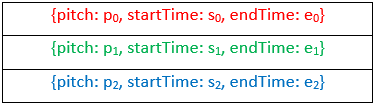
\includegraphics[width=0.35 \linewidth]{image/MIDIState.png}
  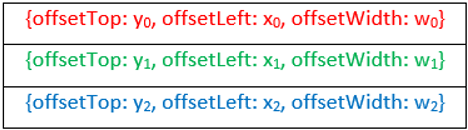
\includegraphics[width=0.35 \linewidth]{image/PositionState.png}
  \includegraphics[width=0.2 \linewidth]{image/RollState.png}
  \caption{A visual synthesis of the three data representations of the MIDI}
  \label{fig:states}
\end{figure}

\paragraph{Save}

The save function saves the current piano roll configuration into a positional sequence; when the
piano roll is reset, it will revert to the most recently saved state.

\begin{lstlisting}[language=JavaScript, label={lst:note_to_seq}, caption={Reading the piano roll configuration into a positional sequence}]
  sequence = []
  for (let note in notes) {
    sequence.append({offsetTop: note.offsetTop,
                     offsetLeft: note.offsetLeft,
                     offsetWidth: note.offsetWidth});
  }
\end{lstlisting}

\paragraph{Reset}

The reset function loads the saved state and converts the MIDI data back into a piano roll
configuration. To start, it deletes all the existing notes. Then it simply repopulates the piano
roll using the same steps the application originally used to convert the default melody when it was
initially opened.

\begin{lstlisting}[language=JavaScript, label={lst:seq_to_note}, caption={Generating a piano roll configuration from a positional sequence}]
  for (let elem in sequence) {
    var newNote = document.createElement('BUTTON');
    newNote.classList.append('note');
    roll.appendChild(newNote);
    newNote.style.top = elem.offsetTop + 'px';
    newNote.style.left = elem.offsetLeft + 'px';
    newNote.style.left = elem.offsetWidth + 'px';
  }
\end{lstlisting}

\paragraph{Undo}

Whenever an interaction is made in any edit mode, before any changes are made to the notes, the
current positional sequence is saved to a queue in the application’s backend. This process of
saving the state uses the same conversions as the save function. When the undo function is called,
it pops a state off the queue and converts the MIDI data back into a piano roll configuration using
the same conversions used by the Reset function. Additionally, when states are saved to the queue
and the queue is at length 10, it will shift before pushing the new state into the queue. This
limits the user’s number of successive reversions to 10, after which the undo button will be
disabled until new edits are made to repopulate the queue. This limitation was imposed to prevent
the application from having to store an infinite number of states into memory. Because we are
operating on standalone hardware, memory is limited and must be consumed shrewdly.

\paragraph{Redo}

Whenever the undo function is called, before the piano roll state is reverted, its positional
sequence is saved to a second queue. This queue behaves much like that used by the undo function.
When the redo function is called, it pops a state off and translates it onto the piano roll.
However, whenever any edit is made besides a call on the undo function, the redo queue empties
itself and is disabled until the undo function is called.

\paragraph{Expand}

The expand button is the button at the end of the piano roll labeled simply with a “+.” Clicking
this button expands the piano roll and populates a new measure grid. The measures are a series of
in-line div elements alternating between 0.3 and 0.4 opacity, each internally formatted with the
CSS grid layout. The application uses a set of for loops to populate each grid with 4 columns and
128 rows, with each row matching the color of the corresponding piano key.

\paragraph{Play}

Finally, we get to discuss MIDI playback. We used the ToneJS library both to achieve the maximally
precise scheduling from JavaScript and to create a synthesizer with a realistic piano sound.
Our synthesizer was created using the ToneJS Sampler. We downloaded a virtual piano from the free
Spitfire Audio LABS library, and recorded that to create MP3 files of the piano playing the C4, E4,
G4, and B4 keys. We then created a new Tone Sampler with the C4, E4, G4, and B4 notes mapped to the
respective MP3 files. From there, ToneJS generated the rest of the synthesizer by shifting the pitch
of the given audio samples until it encompassed the full MIDI range.

The playback process begins by reading the piano roll back into a MIDI sequence. The application
then iterates through the MIDI data, and for each note, schedules an event for the synthesizer to
play the given pitch at the given start and end times.

\begin{equation} \label{get_pitch}
  pitch_{note} = \frac{(height_{note} + key\:gap) * (num\:keys - 1) - top_{note}}{height_{note} + key\:gap}
\end{equation}

\begin{equation} \label{get_start}
  start\:time_{note} = \frac{left_{note}}{measure width} * \frac{tempo}{60}
\end{equation}

\begin{equation} \label{get_end}
  end\:time_{note} = start\:time_{note} + \frac{left_{note}}{measure width} * \frac{tempo}{60}
\end{equation}

The pitch of the note ranges from 0 to 127, as do the virtual keys in the DAW.
Subtracting the top position of the note shows the pixel
distance between the selected note and the bottom note. This is then divided by the unit size of the
note (plus key gap) to determine the number of keys between the note and the base note. This number
translates directly to the integer value of the note's MIDI pitch.

The start time of the note is calculated first by converting the pixel measurement left position
of the note into some decimal number of whole notes. The tempo is then converted from beats per
minute to beats per second. The two converted numbers are multiplied to get the start time in
seconds.

The end time of the note is offset by the start time, then uses the same pixel-to-note-value and
tempo-to-time conversions to determine the duration.

\subsubsection{Programming the Arduino Controller}

Our MIDI keyboard was designed with an intermediary in mind, between the raspberry Pi and
the physically designed circuit of the keys. This intermediary was determined by the
number of inputs, affordability, power consumption, as well as an ability for Serial
communication across USB. Naturally, we did not need a controller with a large number of
pins as we had reduce that requirement when designing the circuit itself. Thusly, we
decided upon the Arduino Nano Every to program and test our build. In the course of
events, we needed to solder more wires onto the controller, but since it would become and
integrated piece of our project it was a necessary expense. It should be noted that the
Raspberry Pi will need to be programmed to accommodate the signals and subsequently react
whenever a new signal is transmitted.

For the Pins and the Serial port itself, only a few small setups needed to take place.

\begin{figure}[h!]
  \centering
  \includegraphics{image/arduinosetups.png}
  \caption{Setup code for the Arduino pins and serial port.}
\end{figure}

The arrStatus array holds the on or off status of each individual key. For our 29 key
keyboard, we needed and array of size 29. The values of Out1 and Out2 hold the digital pin
of the output, allowing the easy change and modification of which pins are being listened
to for each part of the program. As for the output pins, they’re only called here and in a
subsequent function beneath the main loop. If necessary, it’s not terribly difficult to
change which pins correspond to which Serial values within the circuit. The function in
question follows bitwise operations to determine the correct response to each given key
query.

\begin{figure}[h!]
  \centering
  \includegraphics{image/setserialfun.png}
  \caption{Setting the serial function using bitwise operations.}
\end{figure}

This allows each pin to correspond to the correct binary value and for the controller to
easily switch to any key that needs to be listened to at any given moment.

As for the program itself, our query logic follows a loop, and that loop follows a series
of three possible events. These events were considered and programmed for to accommodate
for incomplete connections or potential faults within the circuit. For the purposes of the
program and for the reader’s sake, the first series of buttons(SW1-29) will be called the
back buttons and the second series of buttons(SW33-61) will be called the forward buttons;
corresponding to their location on the physical PCB. First, a loop is created to begin
counting from 0 to 29, utilized to allow for the assignment and signal of the status and
velocity value of the corresponding key being measured. A delay of 1ms is inserted after
calling the above set serial function to ensure that the signal is allowed to propagate
through the circuit and retrieve the correct value of a given key. Then, each of the three
possible events are checked for to determine what action is to take place.

The first event requires the most calculation and logic to implement correctly. If the
back button of a particular key is detected as on, then the time in milliseconds is
measure, corresponding to the time\_1 and time\_2 values below. The state of the status
array is then updated and a nested loop begins, waiting for the on signal in the front
button to occur to accurately measure the difference in time.

\begin{figure}[h!]
  \centering
  \includegraphics{image/pinreadingvelocity.png}
  \caption{First attempt at pin reading code with the velocity calculation.}
\end{figure}

However, as can be noted, there is an additional if statement within the loop to ensure
that the controller will not freeze on a faulty key. This is accomplished by taking
another measure of milliseconds and breaking the loop if the time elapsed exceeds a
quarter of a second. This is the point at which the minimum value of the calculation is
all but guaranteed and therefore becomes a moot point to wait any longer for the signal to
come from the front button of the key. With that check out of the way, the velocity of the
difference in time is then calculated, initially ascribed the float state and then the on
signal is generated and sent over the Serial connection.

With that check out of the way, the velocity of the difference in time is then calculated,
initially ascribed the float state and then the on signal is generated and sent over the
Serial connection.

The number of the key signaled as well as the velocity found is also sent, completing the
first potential signal transmitted to the Raspberry Pi. The only thing left is to scan the
keyboard again and determine if additional keys need to be signaled. This is what’s
typically known as a chord, when multiple keys are pressed in the same instance to
generate a wider variety of songs and melody when playing an instrument. This is
accomplished with another nested loop, this one borrowing the first calculated velocity
and sending it along the Serial port to the Raspberry Pi as well. As can be noted, the
setSerialFun is utilized throughout the loop and the status array is updated when the
correct conditions are met. Once all of that is completed the break; function is called,
resetting the first loop to the beginning, and completing the first potential event of our
program. Fortunately, this is most of the work out of the way as there are only so many
conditions that can be measured for if the back buttons are inexplicably faulty.

The second event is a contingency event, in the case that the first button did not signal
correctly, but the second button was already pressed. In this case, we cannot reverse time
and determine the correct velocity of the given keypress. Thusly, we must make an
assumption and signal the Raspberry pi with a default value that is high enough in
velocity but not too high as to sound impossible. Thusly, a default value of 80 was
decided, but other default values can be utilized.

\begin{figure}[h!]
  \centering
  \includegraphics{image/backupfunction.png}
  \caption{Contigency code for when first button does not signal.}
\end{figure}

Once again, the nested loop is to check if any other buttons may have been pressed while
preoccupied with the signaling of the serial port and subsequently signaled in kind,
updating the status array to reflect which keys are and not pressed at that given moment.
Once again, this function is only ever called when the back button is inexplicably faulty,
and the front buttons still signal correctly. However, the point of being an engineer is
to determine a faulty scenario and create a contingency to mitigate that fault.

The third event is the simplest. Assuming that neither the back nor front buttons are
signaled as high during their measurement but the status array is found to have noted this
note as on before this time, then an off signal must be signaled to the Raspberry Pi.

\begin{figure}[h!]
  \centering
  \includegraphics{image/backupfunction.png}
  \caption{Code to send off event over serial port.}
\end{figure}

An off signal, the key number, and then an empty value is sent across the Serial
connection. Then the status array is updated to reflect the new state of the keyboard.
This is the last event measurable with our current hardware and means of measuring the
circuit signals. This is also the completed program for our Arduino controller that allows
us to properly signal and measure the state of the MIDI keyboard. This program can be
modified and theoretically improved upon to better implement any sized MIDI keyboard
needed. For simplicity’s sake, a key number and value is the only significant means which
the Arduino communicates with the Raspberry Pi. This program can be modified to signal in
the proper MIDI format, but I was far too ignorant of the actual format to attempt to
write code to implement such a state.

\subsection{Testing}

\subsubsection{DAW}

Because there is no way of measuring performance of the DAW, testing it was difficult. Simply, the
quality of the DAW is largely based on the look and feel of it, as well as its ability to handle
edge cases. However, there is no way of simply knowing what edge cases there are, especially for
an application with so many moving parts. Our ultimate method of testing was to collect feedback
from beta test groups. We selected from two demographics for our test. Those in the first group
had sufficient experience producing music using DAWs, and those in the second group were relatively
new to MIDI production. Their task was to experiment with the functionality of the DAW and try to
find edge cases by using unconventional methods. Additionally, they were asked to report back on
the intuitiveness of the user interface.

\subsection{Evaluation}

\subsubsection{DAW}

After receiving feedback from our test group, we have found that the overall look and feel of the
DAW has achieved sufficient polish. The UI design is clean and the fluidity of interactions is
comparable to other simple browser-based DAWs, such as Soundtrap.

\begin{figure}[h!]
  \centering
  \includegraphics[width=\linewidth]{image/Soundtrap.png}
  \caption{A snapshot of the Soundtrap MIDI editor displaying the \textit{Twinkle, Twinkle, Little Star} melody.}
  \label{fig:soundtrap}
\end{figure}

Our test group did manage to find edge cases regarding the snap-to-grid functionality in the use
of the move edit mode. Because the snap moves the note after centering it under the mouse, if the
quantized unit size is large enough, the note is occasionally not under the cursor. In the
click-to-place version of the move function, if the user clicks in this condition, the note will
release its on-mouse-move function making it static but not exiting the move mode. When this
happens, the user will no longer be able to interact with any of the notes until they click the
note they had originally selected. If the user cannot remember which note that is, they can get
stuck on a frozen piano roll. The final iteration of this project will address this issue by only
making the note snap to position if the cursor is within a note-width of a grid marker.

Other test sessions found that the transition of states between the state functions is flawed.
Occasionally, the "Undo" and "Redo" buttons would disable when they should have been enabled. This
issue will be addressed in the final version by refactoring the flow of saved states between the
functions.

Our test group also remarked on quality-of-life features that could be added to improve the user
experience. For example, a time scroller which allows the user to manually skip backward and
forward in MIDI playback. Another suggestion was to have the notes and guide keys play a
one-second sample of the note when clicked so that the user can get an idea of the melody they
are constructing. It was also suggested that the piano roll could include vertical markers that
show where each quarter-/half-/whole-note increment lies, similar to what Soundtrap implements in
\textit{Figure \ref{fig:soundtrap}}.

\begin{figure}[h!]
  \centering
  \includegraphics{image/Scroller.png}
  \caption{An example of a DAW time scroller.}
  \label{fig:scroller}
\end{figure}

In response to this feedback, we fine-tuned our state functions and implemented a time scroller.
The time scroller is animated through a callback function during audio playback. For every frame,
it reads the time in playback from the ToneJS context and moves the time scroller to the
corresponding horizontal location on the piano roll. Additionally, when the piano roll is
translated to a MIDI sequence before playback, any notes located left of the time scroller are
skipped, and all notes have the time offset marked by the time scroller subtracted from their start
and end times. This creates the effect of having the audio start at the point indicated by the time
scroller.

\begin{figure}[h!]
  \centering
  \includegraphics[width=\linewidth]{image/FinalUI.png}
  \caption{Our final UI layout, once again displaying the \textit{Twinkle, Twinkle, Little Star} MIDI}
  \label{fig:soundtrap}
\end{figure}

\subsubsection{AI}

After the model is trained and test, there will be an evaluation benchmark of the AI. For
this well known data sets will be run and compared against pre-trained models provided on
Magenta framework. We could try to develop a deterministic technique fo revaluation,
measuring the percentage of key notes the model can predict from a known case. Although,
this is an objective measurement of the model performance, maybe not fully desirable to
obtain such a grade of regularity on the output, and some stochastic variables can be
added in order of adding elements of unpredictability in the generation of new melodies.

\subsubsection{Programming the Arduino controller}


\section{Equipment}
\subsection{Button Triggers}
To accurately observe the approximately-linear motion of a piano key, we feel a linear push-button switch is our best choice. We do not want any sort of locking mechanism because the key should be registered as ‘on’ when pressed and ‘off’ when released and each key will need two switches, which is a total of sixty-two total switches in the keyboard keys alone. Linear push-button switches provide this linear on-off response and come with a low price tag.

Since we want our project to feel as close to a professional MIDI controller as possible, we do not want our user to know there is a button being actuated separately from the key. This means our buttons should be almost silent and not provide any tactical feedback. To achieve these parameters we did our research and brought three types of buttons to debate: the \textit{Odseven Soft Tactile Button}, the \textit{Panasonic ESE-20d443}, and the \textit{Nidec Copal TR1-01}. The three choices offered are a single-pole single-throw linear push-button with a silicon cover. Their images and data are shown in \textit{Figure \ref{fig:buttons_fig}} and \textit{Table \ref{Tab:buttons_data}} .

\begin{figure}[h!]
  \centering
  \includegraphics[width=\linewidth]{image/Buttons.png}
  \caption{A comparison of button options.}
  \label{fig:buttons_fig}
\end{figure}

\begin{table}[h!]
  \centering
  \resizebox{\textwidth}{!}{%
    \begin{tabular}{|l|l|l|l|}
      \hline
      Brand                           & Cost   & Quantity & Form Factor               \\ \hline
      Odseven                         & \$1.17 & 10       & 7.8mm x 7.8mm x 4.9mm     \\ \hline
      Nidec Copal Electronics         & \$0.54 & 1        & 5.9 mm x 7 mm x 9 mm      \\ \hline
      Panasonic Electronic Components & \$1.31 & 1        & 7.9 mm x 7.8 mm x 17.5 mm \\ \hline
    \end{tabular}}
  \caption{A comparison of costs for our button options.}
  \label{Tab:buttons_data}
\end{table}

After debating which option would be the best for this project, we ultimately settled on the \textit{Odseven Soft Tactile} button for a few reasons. First, as we can see in \textit{Figure \ref{fig:buttons_fig}} and the accompanying \textit{Table \ref{Tab:buttons_data}} , The \textit{Nidec} and the \textit{Panasonic} buttons extend at least twice as high as the \textit{Odseven}. Although the taller buttons could provide more constant contact with the key and reduce the feeling of multiple actuations, the button would need to be in constant contact during the entire actuation of the key to make a difference in feel. On top of that, to receive information for velocity, we would need to place the buttons in different locations on the key and have different actuation distances from the key for each button. No matter our choice, constant contact would require two different types of buttons. Plus, the total actuation of the key is ten degrees for the white keys, fifteen degrees for the black keys, and we would need to find two buttons with extremely precise height and actuating distance.

The next reason we chose the \textit{Odseven Soft Tactile} button was because of the shape of the button itself. With a circular head and smallest actuation distance, it appears to be more versatile for our multistage actuation set-up, where the key is pressed before it presses the button itself. We could use a variety of rod shapes connected to the key and still get the \textit{Odseven} button to actuate properly. This will come in handy during the prototyping and reiteration of the project. It is also versatile enough to be used in other applications of the project, which will be discussed in their personal sections, and because the \textit{Odseven Soft Tactile} button comes in a pack of ten, this adds confidence that we will make the most use of each cent we spend. Additionally, the datasheets provided with all three of these devices do not offer a decibel reading of the button response. The only button which discussed sound was the \textit{Odseven} which claims to be “silent”. From our experience as musicians, we would much rather take a key that has an odd feeling when pressed over a key that clicks when pressed.

The final reason we chose the \textit{Odseven} button is the price. We have a budget goal of below five-hundred dollars and \textit{Odseven} sells this button, as well as \textit{Adafruit}, at a significantly lower price per button than the other options. Our project will be using sixty-four buttons in the keys alone and every unnecessary dollar spent on buttons will add up quickly.

\subsection{Springs}
By utilizing the measurement function of Solidworks we know that the minimum distance the spring will connect is 34.02 mm, shown in \textit{Figure \ref{fig:dimensions1}} and the maximum distance is 38.94 mm shown in \textit{Figure \ref{fig:dimensions2}}.

\begin{figure}[h!]
  \centering
  \includegraphics[width=\linewidth]{image/Dimensions1.png}
  \caption{A close-up on our keys' manufacturing specifications.}
  \label{fig:dimensions1}
\end{figure}

\begin{figure}[h!]
  \centering
  \includegraphics[width=\linewidth]{image/Dimensions2.png}
  \caption{A close-up on our keys' manufacturing specifications.}
  \label{fig:dimensions2}
\end{figure}

From our knowledge of basic kinematics, we know that the force of a spring can be approximated by the equation:

\begin{equation} \label{spring_force}
  F = -k * x
\end{equation}

Where $ F $ is the force in Newton-meters, $ k $ is the spring constant determined by the manufacturing design and material of the spring, and $ x $ is the linear distance from the resting point (or state of equilibrium) of the spring. It is important in our design that the spring remains in tension while the key is at a zero degree actuation all the way to the 15 degree (or 10 degree for the natural keys) actuation. The reason this is important is to create a more even feel to the normal force while actuating the key. For example, if the $ x $ distance from equilibrium is the zero degree, or resting position, of the key, the force on the key would be zero when the key is not being used. Any amount of change in the position would create infinitely more force than its resting position. As Newton’s Third Law states, “for every action (force) in nature there is an equal and opposite reaction”, meaning that in our circumstance, the full actuation of the key will produce infinitely more force than its resting position as felt by the spring and the user pressing the key. Our aim is to allow the actuation of the key to feel as uniform as possible and since the force relationship with the spring’s distance is approximately linear, the percentage change per equal distance actuated is inversely proportional to the starting position of the key, $ x_{intial} $ . To gather a better understanding, this is a more realistic example.

Obviously if the spring is starting at rest any distance traveled from rest would create infinitely more force than when it is at rest. Now, using the keys as a perfect example, let’s say the max actuation distance is a fixed value. In our case, the maximum actuation for any of our keys is 4.92 mm. For example purposes, let’s say the constant value $ k $ is equal to one. If this key is starting at an initial $ x $ value of 1 mm and traveling to 5.92 mm (the maximum actuation distance plus the initial position), the initial force would be 1m Nm and the final force would be 5.92 m Nm. This is a 492\% change in force over the course of the actuation. If the key starts the spring at $ x $ equals 10 mm and finishes at 14.92 mm, the starting force would be 10 m Nm and the final force would be 14.92 m Nm, creating a 49.2\% change in force over the actuation of the key. We can see how the starting position of the spring affects the overall force change over distance in \textit{Table \ref{Tab:x_force}}.

\begin{table}[h!]
  \centering
  \resizebox{\textwidth}{!}{%
    \begin{tabular}{|l|l|l|l|l|l|l|}
      \hline
      X initial (mm) & Constant K & Max Actuation (mm) & X Final (mm) & Force Initial (m N*m) & Force Final (N*m) & Force \% Change \\ \hline
      5              & 2          & 4.92               & 9.92         & 10                    & 19.84             & 98.4            \\ \hline
      10             & 2          & 4.92               & 14.92        & 20                    & 29.84             & 49.2            \\ \hline
      20             & 2          & 4.92               & 24.92        & 40                    & 49.84             & 24.6            \\ \hline
      30             & 2          & 4.92               & 34.92        & 60                    & 69.84             & 16.4            \\ \hline
      50             & 2          & 4.92               & 54.92        & 100                   & 109.84            & 9.84            \\ \hline
      100            & 2          & 4.92               & 104.92       & 200                   & 209.84            & 4.92            \\ \hline
    \end{tabular}}
  \caption{The tabularized relationship between stretch and tension in a spring.}
  \label{Tab:x_force}
\end{table}

From the table it is obvious that, with a fixed maximum actuation, the percent change in force per $ x $ distance is inversely proportional to the initial $ x $ location.

Although this information is valuable and shows the important aspect that we should be wary of the force percent change over distance, it is also important to take into consideration the strength of the material as well. In an ideal world, aiming for a zero percent change in force over distance would mean starting the initial $ x $ value at an infinite distance from its equilibrium. This is obviously not possible as the spring would break long before an infinite distance. We do not have to worry about starting at an infinite distance and we also recognize that the plastic holding the spring will break long before a metal spring breaks, but we do need to take into account the possibility of the spring deforming by being stretched too long. Therefore, creating the best initial distance to reduce the percent change of force over distance is a balance act with the material properties of the spring itself.

Since we do not have any members with mechanical engineering experience on our team, we are more or less, attempting to do this by trial and error. Obviously we are utilizing common sense to make our decisions, but we find it difficult to justify all of our choices through complete objective reasoning. We decided to debate between six different types of springs under the following pretenses. First, the resting position should be less than the zero degree actuation distance of the key. Second, the starting force of the spring should be approximately one pound per square inch. Third, the maximum distance of the spring should not be below the maximum actuation distance necessary. By utilizing trusted websites our group decided on debating the springs shown in \textit{Table \ref{Tab:spring_brand}}.

\begin{table}[h!]
  \centering
  \resizebox{\textwidth}{!}{%
    \begin{tabular}{|l|l|l|l|l|l|l|}
      \hline
      Brand         & Cost    & Quantity & Initial Length & Max Length & Pounds per Distance & Starting Load \\ \hline
      McMaster-Carr & \$13.80 & 2        & 30.2 mm        & 58.1 mm    & .241 lbs/mm         & 1.08 lbs      \\ \hline
      McMaster-Carr & \$12.35 & 2        & 30.6 mm        & 49.2 mm    & .319 lbs/mm         & 1.49 lbs      \\ \hline
      McMaster-Carr & \$10.90 & 2        & 31 mm          & 53.6 mm    & .13 lbs/mm          & .7 lbs        \\ \hline
      WB Jones      & \$3.08  & 1        & .875 inch      & N/A        & .8 lbs/in           & .15 lbs       \\ \hline
      WB Jones      & \$3.08  & 1        & 1 inch         & N/A        & 0.67 lbs/in         & 0.15 lbs      \\ \hline
      WB Jones      & \$2.33  & 1        & 1 inch         & N/A        & 1.38 lbs/in         & .26 lbs       \\ \hline
    \end{tabular}}
  \caption{A comparison of costs for our spring options.}
  \label{Tab:spring_brand}
\end{table}

Although the WB Jones offers cheaper options, it is more difficult to distinguish which spring would be appropriate as they do not provide a maximum length nor any type of image to distinguish the proportions of the springs. Before coming across any of these options, we made sure each selection was a corrosion resistant tension spring equipped with a hooked end to easily be incorporated to our project. Due to the lack of concrete imagery for the references we ultimately decided to focus on the McMaster-Carr options. Images of those options are as follows: the 30.2 mm spring, the 30.6 mm spring, and the 31 mm spring in \textit{Figure \ref{fig:springs}} each provided by McMaster-Carr.

Since we are unaware of the mechanical properties associated with the diameter of the spring wire, the actual feel in the implementation of the pounds per inch or millimeter, or the utilization of a spring in this mechanical system, we are going to decide by approximate parameters and look of each spring. To play it safe, we are choosing to initially purchase the spring which has the least amount of lbs/m. There is no reliable documentation on exactly how much force it takes to compress a piano key and therefore we will be attempting trial and error during the second semester of this project to find the best spring load.

After evaluating the cost and difference of each type of spring, we ended up using a 2.5 in x .25 in x .035 in zinc plated extension springs to create the actuation. These were purchased from Ace Hardware and cost significantly less than any of the previous options.

\newpage
\begin{figure}[h!]
  \centering
  \includegraphics[width=0.6\linewidth]{image/Spring1.png}
  \includegraphics[width=0.6\linewidth]{image/Spring2.png}
  \includegraphics[width=0.6\linewidth]{image/Spring3.png}
  \caption{A comparison of our spring options.}
  \label{fig:springs}
\end{figure}
\newpage

\subsection{Key Rail}

As discussed in the \textbf{Prototyping} subsection of \textbf{Implementation}, we are no longer attempting to 3D print the rail itself. To replace this 3D printed rail, we bought three alternatives to discuss and debate shown in \textit{Table \ref{Tab:rail_brand}}.

\begin{table}[]
  \centering
  \begin{tabular}{|l|l|l|l|l|}
    \hline
    Brand  & Cost    & Quantity & Form Factor  & Material        \\ \hline
    Amazon & \$11.89 & pack     & 1/8 inch     & 'Natural Wood'  \\ \hline
    Amazon & \$5.99  & 2        & 4mm x 300 mm & Stainless Steel \\ \hline
    K\&S   & \$7.14  & 3        & 4mm x 300 mm & Brass           \\ \hline
  \end{tabular}
  \caption{A comparison of material costs for key rail options.}
  \label{Tab:rail_brand}
\end{table}

At the beginning of the discussion, we immediately eliminated the option of the ‘Natural Wood’ dowels. Our aim is to create a device that is not only functional, but also robust and can handle the perturbations that come along with a portable device. Wood cannot handle nearly as much force as metal and it is difficult to even compare that type of wood with the other options because there was little descriptive information on the type of wood other than ‘natural’.

When comparing the Stainless Steel rods to the Brass rods, this choice was difficult. They are both 4 mm x 300 mm which is wonderful for our application, they both ship from Amazon prime which means we would not have to worry about delivery time, they both are consistently in stock, and they are both close enough in price that it is negligible. To decide, we first took a look at the strength of each rod.

According to material-properties.org the yield strength of brass is about 95 MPa, where the yield strength of stainless steel is about 170 MPa. Next we discussed the properties of each metal over time. As brass continues to be used and exposed to the elements it begins to oxidize, or rust, quickly to a greenish-blue material. Stainless steel does not oxidize. Although this factor is not too difficult to address, it is important to recognize that a rusted material has a higher coefficient of friction over its non-rusted counterpart. If we want the keys to continue actuating over time with as little degradation in actuation ease, it is important that the rod which the key is actuating over does not increase in friction over time. It is worth noting that stainless steel does in fact wear down, but the lack of rust will keep the actuation in better condition than if the rod actuated. For these reasons, we felt it was best to choose the 4 mm x 300 mm stainless steel rod for our project.

\subsection{Display}

While debating on which screen to use, our group came up with two options, shown in \textit{Table \ref{Tab:display_brand}}.

\begin{table}[]
  \centering
  \begin{tabular}{|l|l|l|l|}
    \hline
    Brand   & Cost    & Quantity & Display Size \\ \hline
    Newsoul & \$84.99 & 1        & 7 inch       \\ \hline
    ElecLab & \$49.90 & 1        & 5 inch       \\ \hline
  \end{tabular}
  \caption{Comparison of display screen options.}
  \label{Tab:display_brand}
\end{table}

We were torn between utilizing a physical button oriented user interface and a touch screen oriented interface. As a group, we decided that allowing our end-users the option of a touch screen is more up-to-date with current technology. Not only that, the members of our CS division for this project felt the design and creation of a touch based user interface would be easier to code on the backend and easier to operate on the user’s end. Because of this, we eliminated the choice of any non-touch screens for this project. Next, we discussed whether a capacitive or resistive touch screen would be more appropriate. A general rule of thumb for touch screens is: capacitive touch screens are often more expensive, but offer multi-point touch recognition. Resistive touchscreens are often cheaper, but only allow single-point navigation. We felt resistive touch screens are outdated and decided that adding the extra cost of a capacitive touchscreen for the design would be worth the ease of use and a more professional feel to the finalized product.

We also wanted to make sure there was enough room on the screen for the user to easily view the software user interface and be able to navigate the software. Sadly, none of the options offered by the group had a datasheet reliable enough to find the power usage of the screen. Luckily, each screen is designed to be operated by a Raspberry Pi and claims to work well with the device, therefore we can be assured that the current usage is within the limits a Raspberry Pi can offer. This is later discussed in the Batteries section of this paper. Ultimately, we decided to choose the seven-inch display to offer the greatest experience for our end users that fits within our budget.

\subsection{Octave Up/Down}

With almost every electric keyboard there is a trigger on the device for Octave Up and Octave Down. These buttons simply take the input for each key and represent it as the corresponding note in either the octave above that key or the octave below that key. For example, when octave up is triggered, a key that is usually represented as a C in the 1st octave would be sent to the device as a C in the 2nd octave. Octave down shifts the key in the other direction such that a key in the 1st octave would be sent to the device as a key in the 0th octave. It is important to note that there are about 11 octaves in the audible hearing range from C-1 with a frequency around 8 Hz to B10 with a frequency around 31 kHz. The pitch names, MIDI corresponding values, and frequencies can be seen in \textit{Table \ref{Tab:note_frequency}}. Due to the range of octaves and the fact that our keyboard will only have two and half octaves present, it is to be expected that the octave up and octave down buttons should have the option to be pressed multiple times and add additional octave shifts in the specified direction.

\begin{table}[]
  \centering
  \resizebox{\textwidth}{!}{%
    \begin{tabular}{l}
      \includegraphics{image/NoteFrequency}
    \end{tabular}}
  \caption{The tabularized relationship between MIDI values and their tonal frequency.}
  \label{Tab:note_frequency}
\end{table}

In between the Octave Up and Octave Down buttons we will have a single button to play and pause the MIDI notes already inputted into the DAW. This will operate by simply triggering the opposite of which action the playback is currently performing. When paused this button will play the MIDI data, while playing this button will pause the playback of the MIDI roll.

Below the Play / Pause button will be a Record button. This is used to input MIDI data in real time. After the button is first triggered, it will record all inputs from the keyboard from there after. After the user has recorded what they want, they can press the record button again and the recording will stop and save all MIDI data from the time between the first and second button press.

\subsection{Volume Control}

Almost immediately upon the start of our discussion, we decided that a sliding potentiometer would be best for volume control. Not only is it easy to hook up to any device, like any potentiometer, but it also allows physical and visual feedback of the volume. We plan to use an analog general input output pin (GPIO) directly tied from the potentiometer into the Raspberry Pi. After reading the value of the potentiometer, this will be translated to the volume we expect to produce.

\begin{figure}[h!]
  \centering
  \includegraphics[width=\linewidth]{image/VoltageDiv.png}
  \caption{The voltage divider.}
  \label{fig:voltage_div}
\end{figure}

A potentiometer works by using the concept of a voltage divider which is shown in \textit{Figure \ref{fig:voltage_div}} from electronicclinic.com. There is a $ V_{in} $ supplied by a source, in our case the Raspberry Pi, which is connected to a variable resistor. That variable resistor is connected to the actuating lever which is seen on the outside of the potentiometer. As the lever slides upwards along the potentiometer, the resistance increases and creates a change in the output voltage, which is connected to the actuating lever as well. By knowing the input voltage and reading the output voltage, the device is able to tell from the equation given in \textit{Figure \ref{fig:voltage_div}} where on the slider the lever is located. By using this value, we will translate that the bottom position of the potentiometer is zero output volume and the top position of the sliding potentiometer is full or 100\% volume.

Most musicians who have worked in the synthetic side of music composition or performance have worked with sliding potentiometers in this manner and therefore gives another reason why we, as a team, were drawn to the idea of using a sliding potentiometer over a rotating potentiometer. We easily could have chosen to use a rotating potentiometer, but these are more often used in amplifiers, guitars, and other types of instruments that are not the keyboard. At the end of the day, it all comes down to user preference and our team prefers this decision. We also chose to gather the pack of ten over a single sliding potentiometer because it was not only an easier option over Amazon, but it also provides the components in case we would like to add analog synthetic effects to our device.

The device we chose is the WMCONGCONG 10 kOhm sliding potentiometer. This device provides 1023 data points over the course of its actuation which is more than enough to reduce these data points into volume markers. We chose this device because of the cheap cost of \$14.99 for ten units and the small form factor. It was imperative that the sliding potentiometer fit within the vertical limit of the UI cover for the device. As can be seen in the Keyboard Design section of the document, the slot to the right of the screen which is designed to house this potentiometer is well within our limits and fits aesthetically as well.

We do recognize that the actuating lever for this device is a bit homely, but we were able to design and print a cap for the lever and create a more authentic sliding volume potentiometer feel that many mixers and synthetic instruments use.

\begin{figure}[h!]
  \centering
  \includegraphics[width=0.5\linewidth]{image/Potentiometer.png}
  \caption{WMCONGCONG 10 kOhm sliding potentiometer.}
  \label{fig:potentiometer}
\end{figure}


\subsection{Audio Jack}

The audio jack, also known as the headphone jack or auxiliary jack, is the location where the user can input their headphones to listen to the audio being produced by the Raspberry Pi. There are two major types of audio jacks: mono and stereo. Mono headphone jacks are audio outputs that can only send one audio signal out. This means, if an individual is using headphones, the audio in the right ear will be the exact same audio produced in the left ear. Stereo is the counterpart to mono, and can channel two or more audio signals from a single jack. This means, if all is set up correctly, that the left and right speakers can produce two different signals and create a fuller environment for the listener. This can be further understood in the mechanical drawing shown in \textit{Figure \ref{fig:mono}} and \textit{Figure \ref{fig:stereo}} which are the mono and stereo female drawings respectively.

\begin{figure}[h!]
  \centering
  \includegraphics[width=\linewidth]{image/Mono.png}
  \caption{The mono jack option.}
  \label{fig:mono}
\end{figure}
\begin{figure}[h!]
  \centering
  \includegraphics[width=\linewidth]{image/Stereo.png}
  \caption{The stereo jack option.}
  \label{fig:stereo}
\end{figure}

As you can see from \textit{Figure \ref{fig:mono}} and \textit{Figure \ref{fig:stereo}}, each jack is designed with two different pinouts. The mono headphone jack has only a tip and sleeve pin while the stereo jack has a tip, sleeve, and ring pin to connect to the Raspberry Pi,  each connecting to the corresponding location on the male input jack.

Considering our user interface is more about producing a new type of melody designed by artificial intelligence and machine learning and less about the production value itself, we believe it is best to go with the mono headphone jack. Not only is it cheaper, as seen in \textit{Table \ref{Tab:jack_brand}}, but it is also easier to code, connect, work with, and troubleshoot.

\begin{table}[]
  \centering
  \begin{tabular}{|l|l|l|l|l|}
    \hline
    Brand       & Cost   & Quantity & Form Factor         & Notes  \\ \hline
    Switchcraft & \$2.15 & 1        & 10 mm mounting hole & Mono   \\ \hline
    Switchcraft & \$2.25 & 1        & 10 mm mounting hole & Stereo \\ \hline
  \end{tabular}
  \caption{A comparison of costs for our audio jack options.}
  \label{Tab:jack_brand}
\end{table}

\subsection{T-Cobbler}

One big misfortune about the Raspberry Pi compared to Arduino is that the Raspberry Pi model we chose is not as easily accessible to hardware prototyping as any of the Arduino boards. On the flip side, we still want to be able to connect many different analog devices such as the octave up and octave down buttons as well as the headphone jacks and hopefully speakers by the end of the project. To combat this, our group decided it would be in our best interest to purchase a Pi T-Cobbler Plus -- GPIO breakout board for prototyping. This device costs less than ten dollars and will allow for easier prototyping by connecting the GPIO pins on the Pi to a breadboard, shown in \textit{Figure \ref{fig:tcobbler}}.

\begin{figure}[h!]
  \centering
  \includegraphics[width=\linewidth]{image/TCobbler.png}
  \caption{A sample of our T-Cobbler usage in prototyping.}
  \label{fig:tcobbler}
\end{figure}
\newpage

After prototyping, we simply used the pinout on the Pi to connect the devices.

\subsection{MIDI Translation}
Before recording or playing the note on the Raspberry Pi, we need a device that will be able to interpret the analog signals from the keyboard and translate the keystrokes into MIDI data. After the data is acquired it will be sent via USB to the Pi as a MIDI input, but which device should we use? After a short discussion, our group felt that Arduino or one of the many arduino clones would be our best choice due to its ease of integration and the familiarity our members have working in C code. With the integrated multiplexers in the PCB our MCU (Microcontroller Unit) only needed six digital I/O pins for data, one input for voltage in, and one input for group. The cheapest board models that met this description are the Arduino Nano, Arduino Micro, and Arduino Nano-Every. Here is a quick comparison chart of the following devices with the specs we took into account.

\begin{table}[]
\centering
\begin{tabular}{|l|l|l|l|}
\hline
Device            & Arduino Nano & Arduino Micro & Arduino Nano-Every \\ \hline
Digital I/O       & 22           & 20            & 12                 \\ \hline
USB data transfer & Yes          & Yes           & Yes                \\ \hline
Cost              & \$20.70      & \$18.40       & \$11.90            \\ \hline
\end{tabular}
\end{table}

Ultimately, every board available on the Arduino website has the specifications we need to be able to execute the project. Our choice ended up coming down to cost and keeping the project within budget as best as possible. Even with the cheapest option, we were able to have enough digital I/O pins with an included 8 analog pins.

\begin{figure}[h!]
  \centering
  \includegraphics[width=0.8\linewidth]{image/Pins.png}
  \caption{The set of analog pins available through our Arduino.}
  \label{fig:pins}
\end{figure}

Luckily for us it was necessary to utilize those analog pins for the volume slider since the Raspberry Pi does not have an ADC (analog to digital converter). We also chose this device because it had the smallest form factor of the three. Although each device is relatively small and the size itself would not have impacted the project greatly, we figured every little but counts in a fully portable device.

\subsection{Batteries}

Due to the limited options of batteries that we could reasonably have in our possession during the manufacturing process, one of our CS members felt our best choice was purchasing our device battery from a vape shop. TBy doing this we were able to ensure our device would be in our possession on time, but sadly reduced our variety of options. This endeavor was supported by the rest of the group because vape batteries are used to power heating devices: one of the greater current and watt demanding devices we know of. From the measurements we have of the charging device we purchased, our best option in store were 18650 batteries. These are 2.6 amp hour batteries. 2.6 amp hours is right on the cusp of being able to maintain our 2.5 amp device for about an hour. We used two of these batteries and therefore deduced that we should be able to power our device for around 2 hours on a single charge. This is quite short for a portable device, but it was the best option we were able to possess in our time and charging constraints. These batteries are shown in the figure below.

\begin{figure}[h!]
  \centering
  \includegraphics[width=0.8\linewidth]{image/Batteries.png}
  \caption{The batteries used to power our device.}
  \label{fig:batteries}
\end{figure}

\subsection{Printer Filament}

Since we are using an at-home 3D printer, our choices were limited. None of the members in our group felt comfortable changing the specifications of the device and therefore were limited to the settings already established in the printer. Our choices from the very beginning were Sunlu’s PLA and PLA+ options. Considering the entire model was going to be created with this plastic, we did not want to go with the weaker option. The major difference between PLA and PLA+ is that the PLA+ is advertised as a more durable, more reliable printing plastic. Due to this reason, we bought 3 kgs of PLA+ filament: 2 kgs of black filament and 1 kg of white filament to model a keyboard as accurately as possible.

\newpage
\section{Budget}
\begin{table}[]
  \centering
  \resizebox{\textwidth}{!}{%
  \begin{tabular}{|l|l|l|l|l|}
    \hline
    Brand            & Device           & Cost    & Quantity & Full Cost \\ \hline
    Odseven          & Soft Buttons     & \$1.17  & 7        & \$8.19    \\ \hline
    Switchcraft      & Audio Jack       & \$2.15  & 1        & \$2.15    \\ \hline
    Arduino          & MCU              & \$10.90 & 1        & \$10.90   \\ \hline
    McMaster-Carr    & Springs          & \$10.90 & 16       & \$174.40  \\ \hline
    Amazon           & Keyrail          & \$5.99  & 1        & \$5.99    \\ \hline
    Newsoul          & Display          & \$84.99 & 1        & \$84.99   \\ \hline
    WMYCONGCONG      & Volume Pot.      & \$12.99 & 1        & \$12.99   \\ \hline
    T-Cobbler        & Breakout Board   & \$7.95  & 1        & \$7.95    \\ \hline
    N/A              & Printer Filament & \$75    & 1        & \$75.00   \\ \hline
                     &                  &         &          &           \\ \hline
    Total Before Tax &                  &         &          & \$382.56  \\ \hline
  \end{tabular}}
  \caption{The project budget}
  \label{Tab:budget}
\end{table}

\newpage
\section{Milestones}

\begin{table}[h!]
  \centering
  \resizebox{0.85\textwidth}{!}{%
    \begin{tabular}{|S|L|S|L|L|}
      \hline
      \textbf{Week of... (Monday):} & \textbf{Events}       & \textbf{Document Progress (EOW)} & \textbf{Proposed Events (EE)}          & \textbf{Proposed Events (CS)}        \\ \hline
      January 25th                  & 10 pages due          &                                  & General Research                       & General Research                     \\ \hline
      February 1st                  &                       &                                  & General Research                       & General Research                     \\ \hline
      February 8th                  &                       & 20 pages                         & Final Project Direction                & Final Project Direction              \\ \hline
      February 15th                 &                       & 30 pages                         & Microcontroller Comparison Chart       & AI Model Research                    \\ \hline
      February 22nd                 &                       & 40 pages                         & Key CAD Model                          & AI/Hardware Trials                   \\ \hline
      March 1st                     &                       & 50 pages                         & Component Selection                    & Code Diagrams                        \\ \hline
      March 8th                     &                       & 60 pages                         & Component Selection                    & Learn Required Languages             \\ \hline
      March 15th                    & 75 Pages Due          &                                  & BOM Finalized                          & Learn Required Languages             \\ \hline
      March 22nd                    &                       & 90 pages                         & Order Prototyping Material             & UI Design                            \\ \hline
      March 29th                    &                       & 105 pages                        & PCB Design                             & DAW Design                           \\ \hline
      April 5th                     &                       & 120 pages                        &                                        & DAW Design                           \\ \hline
      April 12th                    &                       & 140 pages                        & Building Prototype                     & Modify MusicVAE Sample               \\ \hline
      April 19th                    & 150 Pages Due         &                                  & Building Prototype                     & Modify MusicVAE Sample               \\ \hline
      \textbf{April 26th}           & \textbf{End of SD1}   & \textbf{}                        & \textbf{Breadboard Prototype Complete} & \textbf{Prototype Software Complete} \\ \hline
      \textbf{Week of... (Monday):} & \textbf{Events}       & \textbf{Document Progress (EOW)} & \textbf{Proposed Events (EE)}          & \textbf{Proposed Events (CS)}        \\ \hline
      May 17th                      & Start of SD2          &                                  &                                        & Refactor Software Design             \\ \hline
      May 24th                      &                       &                                  &                                        & Construct Final Backend              \\ \hline
      May 31st                      &                       &                                  &                                        & Construct Final AI                   \\ \hline
      June 7th                      &                       &                                  &                                        & Construct Final DAW                  \\ \hline
      June 14th                     &                       &                                  &                                        & Product Testing                      \\ \hline
      June 21st                     &                       & Heinrich Presentation            &                                        & Finalize Functionality               \\ \hline
      June 28th                     &                       &                                  &                                        & Clean Up Document                    \\ \hline
      July 5th                      &                       &                                  &                                        & Clean Up Product Features            \\ \hline
      July 12th                     &                       &                                  &                                        & Clean Up Product Features            \\ \hline
      July 19th                     &                       &                                  &                                        & TBA                                  \\ \hline
      July 26th                     &                       &                                  &                                        & TBA                                  \\ \hline
      \textbf{August 2nd}           & \textbf{We are done.} & \textbf{}                        & \textbf{}                              & \textbf{TBA}                         \\ \hline
      \textbf{August 7th}           & \textbf{Graduation}   & \textbf{}                        & \textbf{}                              & \textbf{}                            \\ \hline
    \end{tabular}}
  \caption{Proposed timeline.}
  \label{Tab:milestones}
\end{table}
\clearpage

\input{divisionoflabor.tex}
\section{Project Summary}

\blindtext

\section{Conclusions}

With the design and technical aspects of our project worked out, we are confident that we
can achieve our goal of helping the musician in their battle against writer's block by
creating a portable MIDI controller that can give the musician suggestions. We love having
the opportunity to use AI to help people, rather than to replace them. By helping the
musician complete their work, rather than generate entirely new works, the music will
retain the heart and soul of human creativity. We believe by providing creative assistance
we will help struggling musicians continue pursuing music when they would have otherwise
given up on their musical endeavors.

While there are other products that provide AI assisted music suggestions, we believe that
none of them provide the accessibility that our device will provide. As a standalone
device, this can be given to students or people who lack the computer skills to use a full
fledged DAW on a computer. With the simple DAW-like interface we provide, they will be
able to focus on the music without getting lost in technical details. This will also help
those who are already familiar with modern music production, by providing them with a
device they can use whenever they're stuck on a melody. The music they create on the
device can be imported to the computer when they are done, making the device useful beyond
just educational purposes.

With the research we have done over the past few months, we are in a great position to
make this project a reality. Initially, the prospect of creating this device was daunting,
with several unknowns and unfamiliar technology. But after conducting the research and
going through the design process, we have a sense of clarity and we know that we will be
able to accomplish our goals. We have started prototyping, beginning with setting up the
Raspberry Pi, prototyping the DAW user interface, and experimenting with AI. We are happy
with our technical progress up to this point and will continue develop the project to its
conclusion.

With this document, we have shown that we have considered the legal implications, broader
impacts, worked out the specifications and requirements, conducted thorough research,
worked out the design and implementation details. We have a list of equipment, a budget,
and a list of progress milestones to hold us accountable towards the project's completion.
We hope to have demonstrated with our document that our team has an understanding for what
work needs to be done and a development process to guide us there.

\appendix
\appendixpage

\section{Magenta benchmarks results}
\label{appendix:magenta_benchmark}
\begin{minipage}{\linewidth}
    \captionof{table}{Magenta Benchmark Times (in seconds)}
    \begin{adjustbox}{width=\textwidth}
        \csvautotabular[respect underscore=true]{raspberry_pi_4_magenta.csv}
    \end{adjustbox}
\end{minipage}

\newpage
\printbibliography

\end{document}
